\documentclass[]{book}
\usepackage{lmodern}
\usepackage{amssymb,amsmath}
\usepackage{ifxetex,ifluatex}
\usepackage{fixltx2e} % provides \textsubscript
\ifnum 0\ifxetex 1\fi\ifluatex 1\fi=0 % if pdftex
  \usepackage[T1]{fontenc}
  \usepackage[utf8]{inputenc}
\else % if luatex or xelatex
  \ifxetex
    \usepackage{mathspec}
  \else
    \usepackage{fontspec}
  \fi
  \defaultfontfeatures{Ligatures=TeX,Scale=MatchLowercase}
\fi
% use upquote if available, for straight quotes in verbatim environments
\IfFileExists{upquote.sty}{\usepackage{upquote}}{}
% use microtype if available
\IfFileExists{microtype.sty}{%
\usepackage{microtype}
\UseMicrotypeSet[protrusion]{basicmath} % disable protrusion for tt fonts
}{}
\usepackage[margin=1in]{geometry}
\usepackage{hyperref}
\hypersetup{unicode=true,
            pdftitle={analizaR datos políticos},
            pdfauthor={Francisco Urdinez y Andrés Cruz Labrín (editores)},
            pdfborder={0 0 0},
            breaklinks=true}
\urlstyle{same}  % don't use monospace font for urls
\usepackage{natbib}
\bibliographystyle{apalike}
\usepackage{color}
\usepackage{fancyvrb}
\newcommand{\VerbBar}{|}
\newcommand{\VERB}{\Verb[commandchars=\\\{\}]}
\DefineVerbatimEnvironment{Highlighting}{Verbatim}{commandchars=\\\{\}}
% Add ',fontsize=\small' for more characters per line
\usepackage{framed}
\definecolor{shadecolor}{RGB}{248,248,248}
\newenvironment{Shaded}{\begin{snugshade}}{\end{snugshade}}
\newcommand{\AlertTok}[1]{\textcolor[rgb]{0.94,0.16,0.16}{#1}}
\newcommand{\AnnotationTok}[1]{\textcolor[rgb]{0.56,0.35,0.01}{\textbf{\textit{#1}}}}
\newcommand{\AttributeTok}[1]{\textcolor[rgb]{0.77,0.63,0.00}{#1}}
\newcommand{\BaseNTok}[1]{\textcolor[rgb]{0.00,0.00,0.81}{#1}}
\newcommand{\BuiltInTok}[1]{#1}
\newcommand{\CharTok}[1]{\textcolor[rgb]{0.31,0.60,0.02}{#1}}
\newcommand{\CommentTok}[1]{\textcolor[rgb]{0.56,0.35,0.01}{\textit{#1}}}
\newcommand{\CommentVarTok}[1]{\textcolor[rgb]{0.56,0.35,0.01}{\textbf{\textit{#1}}}}
\newcommand{\ConstantTok}[1]{\textcolor[rgb]{0.00,0.00,0.00}{#1}}
\newcommand{\ControlFlowTok}[1]{\textcolor[rgb]{0.13,0.29,0.53}{\textbf{#1}}}
\newcommand{\DataTypeTok}[1]{\textcolor[rgb]{0.13,0.29,0.53}{#1}}
\newcommand{\DecValTok}[1]{\textcolor[rgb]{0.00,0.00,0.81}{#1}}
\newcommand{\DocumentationTok}[1]{\textcolor[rgb]{0.56,0.35,0.01}{\textbf{\textit{#1}}}}
\newcommand{\ErrorTok}[1]{\textcolor[rgb]{0.64,0.00,0.00}{\textbf{#1}}}
\newcommand{\ExtensionTok}[1]{#1}
\newcommand{\FloatTok}[1]{\textcolor[rgb]{0.00,0.00,0.81}{#1}}
\newcommand{\FunctionTok}[1]{\textcolor[rgb]{0.00,0.00,0.00}{#1}}
\newcommand{\ImportTok}[1]{#1}
\newcommand{\InformationTok}[1]{\textcolor[rgb]{0.56,0.35,0.01}{\textbf{\textit{#1}}}}
\newcommand{\KeywordTok}[1]{\textcolor[rgb]{0.13,0.29,0.53}{\textbf{#1}}}
\newcommand{\NormalTok}[1]{#1}
\newcommand{\OperatorTok}[1]{\textcolor[rgb]{0.81,0.36,0.00}{\textbf{#1}}}
\newcommand{\OtherTok}[1]{\textcolor[rgb]{0.56,0.35,0.01}{#1}}
\newcommand{\PreprocessorTok}[1]{\textcolor[rgb]{0.56,0.35,0.01}{\textit{#1}}}
\newcommand{\RegionMarkerTok}[1]{#1}
\newcommand{\SpecialCharTok}[1]{\textcolor[rgb]{0.00,0.00,0.00}{#1}}
\newcommand{\SpecialStringTok}[1]{\textcolor[rgb]{0.31,0.60,0.02}{#1}}
\newcommand{\StringTok}[1]{\textcolor[rgb]{0.31,0.60,0.02}{#1}}
\newcommand{\VariableTok}[1]{\textcolor[rgb]{0.00,0.00,0.00}{#1}}
\newcommand{\VerbatimStringTok}[1]{\textcolor[rgb]{0.31,0.60,0.02}{#1}}
\newcommand{\WarningTok}[1]{\textcolor[rgb]{0.56,0.35,0.01}{\textbf{\textit{#1}}}}
\usepackage{longtable,booktabs}
\usepackage{graphicx,grffile}
\makeatletter
\def\maxwidth{\ifdim\Gin@nat@width>\linewidth\linewidth\else\Gin@nat@width\fi}
\def\maxheight{\ifdim\Gin@nat@height>\textheight\textheight\else\Gin@nat@height\fi}
\makeatother
% Scale images if necessary, so that they will not overflow the page
% margins by default, and it is still possible to overwrite the defaults
% using explicit options in \includegraphics[width, height, ...]{}
\setkeys{Gin}{width=\maxwidth,height=\maxheight,keepaspectratio}
\IfFileExists{parskip.sty}{%
\usepackage{parskip}
}{% else
\setlength{\parindent}{0pt}
\setlength{\parskip}{6pt plus 2pt minus 1pt}
}
\setlength{\emergencystretch}{3em}  % prevent overfull lines
\providecommand{\tightlist}{%
  \setlength{\itemsep}{0pt}\setlength{\parskip}{0pt}}
\setcounter{secnumdepth}{5}
% Redefines (sub)paragraphs to behave more like sections
\ifx\paragraph\undefined\else
\let\oldparagraph\paragraph
\renewcommand{\paragraph}[1]{\oldparagraph{#1}\mbox{}}
\fi
\ifx\subparagraph\undefined\else
\let\oldsubparagraph\subparagraph
\renewcommand{\subparagraph}[1]{\oldsubparagraph{#1}\mbox{}}
\fi

%%% Use protect on footnotes to avoid problems with footnotes in titles
\let\rmarkdownfootnote\footnote%
\def\footnote{\protect\rmarkdownfootnote}

%%% Change title format to be more compact
\usepackage{titling}

% Create subtitle command for use in maketitle
\newcommand{\subtitle}[1]{
  \posttitle{
    \begin{center}\large#1\end{center}
    }
}

\setlength{\droptitle}{-2em}

  \title{analizaR datos políticos}
    \pretitle{\vspace{\droptitle}\centering\huge}
  \posttitle{\par}
    \author{Francisco Urdinez y Andrés Cruz Labrín (editores)}
    \preauthor{\centering\large\emph}
  \postauthor{\par}
      \predate{\centering\large\emph}
  \postdate{\par}
    \date{2018-11-09}

\usepackage[spanish, es-tabla]{babel} % Andrés: Pone los nombres de tablas, figuras, etc en español. es-tabla hace que sea "Tabla" en vez del horrible "Cuadro" (https://byte77.blogspot.cl/2011/08/no-cuadro-sino-tabla-el-tipico-dolor-de.html).
\usepackage{booktabs}
\usepackage{amsthm}
\makeatletter
\def\thm@space@setup{%
  \thm@preskip=8pt plus 2pt minus 4pt
  \thm@postskip=\thm@preskip
}
\makeatother

\begin{document}
\maketitle

{
\setcounter{tocdepth}{1}
\tableofcontents
}
\hypertarget{inicio}{%
\chapter*{Inicio}\label{inicio}}
\addcontentsline{toc}{chapter}{Inicio}

\hypertarget{capitulos}{%
\subsection*{Capítulos}\label{capitulos}}
\addcontentsline{toc}{subsection}{Capítulos}

\begin{enumerate}
\def\labelenumi{\arabic{enumi}.}
\tightlist
\item
  Prefacio
\item
  Introducción \textbf{I. Introducción a R}
\item
  R Básico (Andrés Cruz Labrín)
\item
  Manejo de datos (Andrés Cruz Labrín)
\item
  Visualización de datos (Soledad Araya)
\item
  Carga de bases y flujo de trabajo (Andrés Cruz Labrín) \textbf{II.
  Modelos}
\item
  Estadística inferencial básica (?)
\item
  Modelos lineales (Inés Fynn y Lihuen Nocetto)
\item
  Modelos binarios (Francisco Urdinez)
\item
  Modelos de supervivencia (Francisco Urdinez) \textbf{III.
  Aplicaciones}
\item
  Estandarización de datos (?)
\item
  Imputación de datos (?)
\item
  Análisis factorial (Caterina Labrín)
\item
  Minería de datos (Gonzalo Barría)
\item
  Análisis de redes (Andrés Cruz Labrín)
\item
  Análisis de texto (Sebastián Huneeus)
\item
  Generación de mapas (Andrea Escobar y Gabriel Ortiz)
\end{enumerate}

\hypertarget{acerca-de-los-autores-y-autoras}{%
\subsection*{Acerca de los autores y
autoras}\label{acerca-de-los-autores-y-autoras}}
\addcontentsline{toc}{subsection}{Acerca de los autores y autoras}

\begin{itemize}
\tightlist
\item
  Gonzalito Barría es un \_\_\_.
\end{itemize}

\hypertarget{prefacio}{%
\chapter{Prefacio}\label{prefacio}}

Este libro nació haciendo análisis de datos políticos. Es decir, es hijo
de la praxis. Por ello su naturaleza es aplicada, y tiene su foco puesto
en ser una caja de herramientas para el lector. \emph{AnalizaR Datos
Políticos} está pensado para ser un manual de referencia que podrá ser
consultado tanto por un estudiante universitario viviendo en Bogotá,
como por un consultor político viviendo en México DF o un o funcionário
público en Brasilia, todos con la necesidad de transformar sus bases de
datos en conclusiones sustantivas y fácilmente interpretables.

Trabajando juntos en la cátedra de Análisis Cuantitativo de Datos II del
Instituto de Ciencia Política de la Universidad Católica de Chile
encontramos que ni aquí, ni en otras universidades de la región, había
material didáctico y aplicado hecho en casa para enseñar a nuestros
alumnos de ciencia política cómo extraer conclusiones a partir de datos
duros. Todo el material utilizado en nuestra cátedra era publicado en
inglés, por politólogos anglosajones trabajando en universidades
anglosajonas. Por ello \emph{AnalizaR Datos Políticos} tiene como
público imaginario al politólogo latinoamericano, ya sea alumno de
pregrado o posgrado, o ya en el mercado. Hemos querido que nuestro libro
esté disponible en español y portugués, y esto lo hace extensible a
otras universidades de realidades similares fuera de América Latina,
como en los países lusófonos de África y en la región ibérica.

Los autores son politólogos que tuvieron que enfrentarse a problemas
aplicados y tuvieron curvas de aprendizaje, más o menos empinandas, en
el uso de \texttt{R}. Agunos han migrado de otros software de análisis
de datos, otros han comenzado su experiencia directamente en \texttt{R}.
Algunos son hábiles usuarios, otros, usuarios funcionales, pero todos
tienen en común que tienen conocimiento aplicado que será de utilidad a
quien quiera tener material de apoyo.

Las universidades latinoamericanas han hecho grandes esfuerzos en que
sus alumnos de politología se alfabeticen en herramientas estadísticas y
de análisis de datos, algo que hasta hace diez años era algo poco
frecuente. Hoy las cinco mejores universidades de la región, según el
ranking de Times Higher Education, tienen cursos de análisis
cuantitativo de datos en sus programas de ciencia política. Algunos
departamentos, como el Departamento de Ciencia Política de la
Universidad de São Paulo, que co-organiza la escuela de verano de IPSA
en métodos, el Instituto de Ciencia Política de la Universidad Católica
de Chile, que organiza su escuela de verano en Métodos Mixtos, o la
División de Estudios Políticos del CIDE, han hecho esfuerzos por exponer
a sus alumnos a profesores norteamericanos y europeos que cuentan con
muchas décadas de tradición cuantitativa en sus programas. Lo bueno es
que poco a poco comienzan a aparecer metodólogos nacidos y formados en
América Latina. Entendemos que, hoy por hoy, ningún politólogo puede
salir al mercado laboral sin saber utilizar con holgura software de
análisis cuantitativo, y es a esa demanda a la que apuntamos aquí.

Ahora mismo, \texttt{R} es probablemente la mejor opción que el mercado
provee para análisis estadístico de datos. Esto puede ser sorpresivo
para un lector recién salido de una máquina del tiempo: hace diez años,
o tal vez menos, R era simplemente mirado como la alternativa gratis a
los programas comerciales de verdad, que sí podían realizar análisis
cuantitativo serio. Sin embargo, esto ha cambiado drásticamente en los
últimos años. La Figura \ref{fig:pref-gtrends} muestra las tendencias de
búsqueda en Google en América Latina para los programas más comúnmente
utilizados en ciencia. \texttt{R} ha pasado a ocupar un lugar en el
mercado que hace 15 años le correspondía a SPSS, y los programas de
nicho -como Stata y Minitab- son cada vez menos buscados. La tendencia
sugiere que \texttt{R} será cada vez más popular en la ciencia
latinoamericana, siguiendo una tendencia global.

\begin{figure}

{\centering 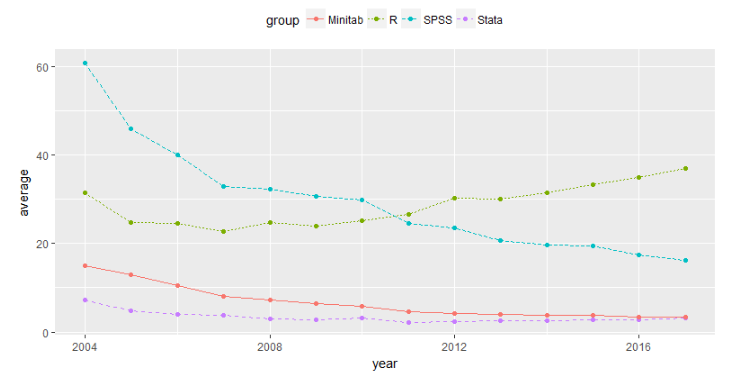
\includegraphics[width=1\linewidth]{00-images/pref-gtrends} 

}

\caption{Elaborada por los autores usando el paquete ggplot2 de R, y datos extraídos de Google Trends. Los datos corresponden a promedios anuales para países latinoamericanos en el sector 'ciencia'}\label{fig:pref-gtrends}
\end{figure}

El modelo de software libre en el que se basa \texttt{R} ---con
licencias de derechos de autor permisivas, que ponen prácticamente todas
las herramientas en forma gratuita a disposición del público, tanto para
su uso como para su reformulación--- finalmente rindió frutos. Una
activa comunidad de desarrolladores se ha anclado en \texttt{R},
añadiéndole nuevas funcionalidades que lo han dotado de elegancia,
simplicidad y flexibilidad. \texttt{R} ya no solo brilla en la
generación de modelos estadísticos, sino que hoy es hogar de un vasto
universo de herramientas que permite al usuario importar, ordenar,
transformar, visualizar, modelar y comunicar los datos que le interesen,
sin tener que cambiar de herramienta.

Es esta la novedad tecnológica que queremos acercar al lector interesado
en el análisis político, con la esperanza de que contribuya a optimizar
el proceso entre la pregunta que le quita el sueño (y/o le promete el
pan) y su solución. Esto sin desconocer, claro está, que el beneficio
inicial de \texttt{R}, el que estaba incluso cuando nadie quisiera
usarlo si no era a regañadientes, permanece. Sabemos que el lector ---y
tal vez su casa de estudios--- agradecerá la amable coincidencia de que
el mejor software disponible en términos de calidad es también el mejor
para su bolsillo.

Francisco Urdinez y Andrés Cruz.

Santiago de Chile, 2018.

\hypertarget{agradecimientos}{%
\section{Agradecimientos}\label{agradecimientos}}

Por ahora nadie. A la concha de tu abuela

\hypertarget{introduccion}{%
\chapter{Introducción}\label{introduccion}}

El análisis cuantitativo de datos es una de las tantas herramientas que
los investigadores tenemos para abordar las preguntas que nos interesan,
ya sea en el mundo profesional o en la academia (o ``por amor al arte''
en muy encendidas noches de viernes, por qué no). Es por esto que
\emph{AnalizaR Datos Políticos} tiene un fuerte énfasis en ejemplos
politológicos aplicados. Utilizar ejemplos de texto trillados e
idealizados sobre autitos o islas imaginarias sería una falta de respeto
para el lector, a quien sabemos ávido por ocupar las herramientas de
este libro en las preguntas de investigación política que le parecen
importantes. Por el contrario, queremos mostrar el potencial de dichas
herramientas metiendo las manos en la masa, con datos de verdad,
investigaciones que colegas ya han realizado y dificultades particulares
de llevar el análisis de datos a preguntas políticas.

\hypertarget{organizacion-del-libro}{%
\section{Organización del libro}\label{organizacion-del-libro}}

El libro está organizado en tres secciones temáticas. Dentro de las
secciones, cada capítulo se esfuerza por resolver problemas puntuales,
balanceando teoría y práctica en \texttt{R}.

 La sección I está dedicada al manejo de datos. Lo ideal es que el
lector consiga algo más que mirar una base de datos con cara de no
entender nada. Introduciremos \texttt{R} desde su instalación y
aprenderemos a sacarle el jugo para obtener datos, conocerlos en
profundidad, transformarlos de acuerdo a las preguntas que nos interesan
y representarlos gráficamente en formas tanto funcionales como
atractivas.

 En la sección II está el corazón del libro. Veremos cómo responder a
preguntas políticas desde una perspectiva estadística ---siempre podemos
contestar desde la perspectiva de lo que nos dijo nuestra abuelita,
aunque esto suela ser menos serio---. En general, la sección trata
modelos estadísticos, que intentan explicar y predecir la variación de
ciertas variables (dependientes) de acuerdo a cómo varían otras
variables (independientes). Exploraremos distintos tipos de modelos de
acuerdo a las distintas formas de variables dependientes que se
encuentran comúnmente en la arena de lo político. Revisaremos cómo
interpretar resultados y presentarlos en forma clara y atractiva, cómo
elegir entre modelos competidores y cómo comprobar simplemente algunos
de los supuestos estadísticos necesarios para que los modelos funcionen.
Debemos notar que este no es un libro de econometría, claro está, por lo
que para cada modelo haremos referencia a trabajos más avanzados en
términos teóricos, con el fin de que el lector pueda profundizar por su
cuenta si cree que debe utilizar algún modelo en específico para
responder a sus preguntas de interés.

 Por último, en la sección III dejaremos el mundo ideal y nos
adentraremos en la resolución de problemas. Ya sea porque un colega nos
prestó su base de datos y se vé más bien como una obra de arte
surrealista, o simplemente porque la dificultad de los problemas a los
que nos enfrentamos deja corto lo que aprendimos al principio del libro,
aquí presentaremos un popurrí de herramientas para que el lector integre
en su flujo de trabajo cotidiano. Estas han sido seleccionadas desde
nuestra experiencia y son cuáles creemos las más requeridas en la
práctica del análisis de datos políticos.

\hypertarget{prerrequisitos}{%
\section{Prerrequisitos}\label{prerrequisitos}}

Este libro está pensado para alumnos que más que brillantes son
motivados: el análisis cuantitativo de datos exige sobre todo tenacidad
y curiosidad. Es altamente deseable que el lector tenga nociones básicas
de matemática, probabilidad y/o estadística universitaria antes de leer
este libro, aun cuando nos esforzamos por mantenerlo lo más simple que
pudimos en dichas materias. En términos de hardware, prácticamente
cualquier computador moderno con acceso a internet será suficiente, pues
las herramientas que utilizaremos son más bien livianas. Todo el
software que utilizaremos es gratuito.

\hypertarget{part-introduccion-a-r}{%
\part{Introducción a R}\label{part-introduccion-a-r}}

\hypertarget{rbas}{%
\chapter{R básico}\label{rbas}}

\hypertarget{instalacion}{%
\section{Instalación}\label{instalacion}}

\hypertarget{r}{%
\subsection{R}\label{r}}

R (R Core Team, 2017) es un lenguaje de programación especialmente
desarrollado para realizar análisis estadístico. Una de sus principales
características, como se ha dejado a entrever en el prefacio, es que es
de \emph{código libre}: aparte de ser gratis, esto significa que las
licencias que protegen legalmente a R son muy permisivas. Al amparo de
esas licencias, miles de desarrolladores alrededor del mundo han añadido
su granito de arena a la usabilidad y atractivo de R. ¡En \emph{analizaR
datos políticos} le sacaremos el jugo a esa diversidad!

Instalar R es fácil, independiente de si el usuario utiliza Windows, Mac
o Linux. Basta con ingresar a \url{https://cran.r-project.org/} y seguir
las instrucciones de descarga a instalación.

\hypertarget{rstudio}{%
\subsection{RStudio}\label{rstudio}}

Como dijimos, R es un lenguaje de programación. En términos informales,
es una forma ordenada de pedirle al computador que realice ciertas
operaciones. Esto significa que es posible usar R exclusivamente desde
una consola o terminal -las pantallas negras de los hackers de las
películas. Aunque esto tiene algunos atractivos -entre ellos, parecer
hacker-, en general queremos interfaces más amigables. Ahí es cuando
entra al ruedo RStudio, el programa de facto para utilizar R. Una vez
esté instalado, todos nuestros análisis ocurrirán dentro de RStudio,
que, para más remate, es también de código libre. Para instalar RStudio,
es necesario ya haber instalado R. Como para este, la descarga e
instalación es accesible en Windows, Mac y Linux. El link es
\url{https://www.rstudio.com/products/rstudio/download/\#download}

Instale ambos R y RStudio, que nosotros lo esperamos aquí.

Será bueno que nos acompañe a lo largo del capítulo con el programa
abierto en su computador, nada mejor que aprender juntos.

\hypertarget{partes-de-rstudio}{%
\section{Partes de RStudio}\label{partes-de-rstudio}}

Si el lector consiguió descargar e instalar R y RStudio, bastará con
ingresar a RStudio para comenzar a trabajar. Se pillará con una pantalla
como esta (\emph{pulir! mejor fuente, fondo blanco}):

\emph{(F:creo que antes de largar habría que explicarle al lector como
cambiar el idioma y ver ese tema del UTF8)}

\begin{center}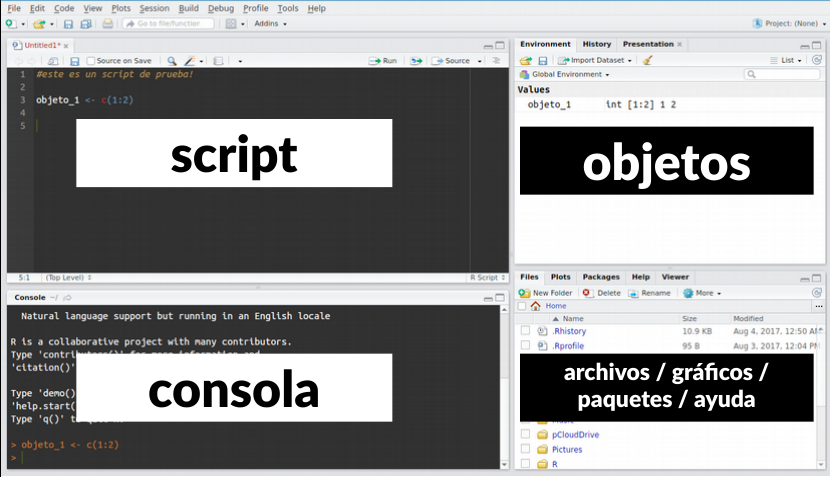
\includegraphics[width=11.53in]{00-images/rbas-rstudio} \end{center}

La pantalla de RStudio se divide en cuatro paneles. A continuación,
vamos a explicar sus funciones. La idea en esta sección es familiarizar
al lector con lo básico de R en el camino.

\hypertarget{consola}{%
\subsection{Consola}\label{consola}}

El panel inferior izquierdo de RStudio. Es nuestro espacio de
comunicación directa con el computador, en el que le solicitamos,
hablando R, realizar tareas específicas. Llamaremos \textbf{comandos} a
estas solicitudes. Probemos correr un comando que realiza una operación
aritmética básica:

\begin{Shaded}
\begin{Highlighting}[]
\DecValTok{2} \OperatorTok{+}\StringTok{ }\DecValTok{2}
\CommentTok{## [1] 4}
\end{Highlighting}
\end{Shaded}

Un truco importante de la consola es que con los botones de arriba y
abajo es posible navegar en el historial de comandos recientes.
Recomendamos al lector probar de realizar otros comandos con operaciones
aritméticas y volver atrás con los botones de arriba y abajo.

\emph{cambiar imagen de resumen}

\begin{center}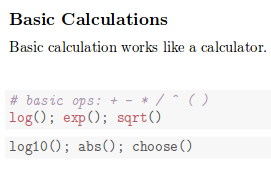
\includegraphics[width=3.76in]{00-images/rbas-basiccalc} \end{center}

Por ejemplo:

\begin{Shaded}
\begin{Highlighting}[]
\KeywordTok{sqrt}\NormalTok{(}\DecValTok{100}\NormalTok{) }\OperatorTok{-}\StringTok{ }\DecValTok{2}\OperatorTok{^}\DecValTok{3} \OperatorTok{*}\StringTok{ }\DecValTok{3}
\CommentTok{## [1] -14}
\end{Highlighting}
\end{Shaded}

\hypertarget{script}{%
\subsection{Script}\label{script}}

El panel superior izquierdo de RStudio puede describirse como una suerte
de ``bitácora de comandos''. Aunque la consola puede ser útil para unos
pocos comandos, análisis complejos requerirán que llevemos un registro
de nuestros comandos.

Para abrir un script nuevo, basta con presionar
\texttt{Ctrl\ +\ Shift\ +\ N} o ir a File \textgreater{} New File
\textgreater{} R Script (utilizar atajos de teclado suele ser una buena
idea, y no solo por el factor hacker \emph{A:footnote al anexo tips?}
\emph{F: Yo creo que puede ir a la Parte III}). La pantalla en blanco de
un nuevo script es similar a un bloc de notas sin usar, con la
particularidad de que cada línea debe pensarse como un comando. El
lector debe notar que escribir un comando en el script y presionar
\texttt{Enter} no consigue nada más que un salto de párrafo. Para correr
el comando de una línea basta con presionar \texttt{Ctrl\ +\ Enter} (en
el caso de Mac, \texttt{Cmd\ +\ Enter}) mientras se tiene el teclado en
ella. ¡Es posible seleccionar múltiples líneas/comandos a la vez y
correrlas de una pasada con \texttt{Ctrl\ +\ Enter}!

Es fundamental el dejar comentarios explicativos en nuestros scripts.
Esto no es solo relevante en el trabajo en grupo (el código ajeno puede
ser inentendible sin una guía clara), sino que también denota atención
por nuestros yo del futuro. En varias ocasiones nos ha tocado revisar
código que escribimos hace un par de meses, no entender nada, y maldecir
a nuestros yo del pasado por su poca consideración. A la hora de
interpretar comandos, R reconoce que todo lo que siga a un numeral (\# o
\emph{hashtag}, en estos días) es un comentario. Así, hay dos formas de
dejar comentarios, como ``comandos estériles'' o como apéndices de
comandos funcionales:

\begin{Shaded}
\begin{Highlighting}[]
\CommentTok{# Este es un comando estéril. R sabe que es solo un comentario, por lo que no retorna nada.}
\end{Highlighting}
\end{Shaded}

\begin{Shaded}
\begin{Highlighting}[]
\DecValTok{2} \OperatorTok{+}\StringTok{ }\DecValTok{2} \CommentTok{# Este es un comando-apéndice. ¡R corre el comando hasta el gato y luego sabe que es un comentario!}
\CommentTok{## [1] 4}
\end{Highlighting}
\end{Shaded}

Para guardar un script, basta con presionar \texttt{Ctrl\ +\ S} o
clickear File \textgreater{} Save.

\hypertarget{objetos}{%
\subsection{Objetos}\label{objetos}}

El panel superior derecho de RStudio. Aunque tiene tres pestañas, la
gran estrella es ``Environment'', que sirve como registro para los
objetos que vayamos creando a medida que trabajamos. Una de las
características centrales de R es que permite almacenar objetos, para
luego correr comandos en ellos. La forma tipo para crear un objeto es
\texttt{nombre\_del\_objeto\ \textless{}-\ contenido}. Por ejemplo:

\begin{Shaded}
\begin{Highlighting}[]
\NormalTok{objeto_}\DecValTok{1}\NormalTok{ <-}\StringTok{ }\DecValTok{2} \OperatorTok{+}\StringTok{ }\DecValTok{2}
\end{Highlighting}
\end{Shaded}

El lector notará que en la pestaña ``Environment'' aparece un nuevo
objeto, objeto\_1. Este contiene \emph{el resultado} de 2 + 2. Es
posible preguntarle a R qué contiene un objeto simplemente corriendo su
nombre como si fuera un comando:

\begin{Shaded}
\begin{Highlighting}[]
\NormalTok{objeto_}\DecValTok{1}
\CommentTok{## [1] 4}
\end{Highlighting}
\end{Shaded}

Los objetos pueden insertarse en otros comandos, haciendo referencia a
sus contenidos. Por ejemplo:

\begin{Shaded}
\begin{Highlighting}[]
\NormalTok{objeto_}\DecValTok{1} \OperatorTok{+}\StringTok{ }\DecValTok{10}
\CommentTok{## [1] 14}
\end{Highlighting}
\end{Shaded}

También es posible reasignar a los objetos. ¡Si nos aburrimos de
objeto\_1 como un 4, podemos asignarle cualquier valor que queramos!
Valores de caracter o no númericos se pueden asignar entre comillas:

\begin{Shaded}
\begin{Highlighting}[]
\NormalTok{objeto_}\DecValTok{1}\NormalTok{ <-}\StringTok{ "democracia"}
\end{Highlighting}
\end{Shaded}

\begin{Shaded}
\begin{Highlighting}[]
\NormalTok{objeto_}\DecValTok{1} 
\CommentTok{## [1] "democracia"}
\end{Highlighting}
\end{Shaded}

Borrar objetos es también muy simple. ¡Aunque suene como perder nuestro
duro trabajo, tener un ``Environment'' limpio y fácil de leer a menudo
lo vale!

\begin{Shaded}
\begin{Highlighting}[]
\KeywordTok{rm}\NormalTok{(objeto_}\DecValTok{1}\NormalTok{)}
\end{Highlighting}
\end{Shaded}

\hypertarget{vectores}{%
\subsubsection{Vectores}\label{vectores}}

Hasta ahora hemos conocido los objetos más simples de R, que contienen
un solo valor. Objetos un poco más complejos son los vectores,
``lineas'' de valores. Crear un vector es simple, basta con insertar sus
componentes dentro de \texttt{c()}, separados por comas:

\begin{Shaded}
\begin{Highlighting}[]
\NormalTok{vector_}\DecValTok{1}\NormalTok{ <-}\StringTok{ }\KeywordTok{c}\NormalTok{(}\DecValTok{15}\NormalTok{, }\DecValTok{10}\NormalTok{, }\DecValTok{20}\NormalTok{)}
\end{Highlighting}
\end{Shaded}

\begin{Shaded}
\begin{Highlighting}[]
\NormalTok{vector_}\DecValTok{1}
\CommentTok{## [1] 15 10 20}
\end{Highlighting}
\end{Shaded}

\hypertarget{funciones}{%
\subsubsection{Funciones}\label{funciones}}

Sin notarlo, hemos ya utilizado a través \texttt{sqrt()}, \texttt{log()}
y \texttt{c()}una de las cualidades más importantes de R, las funciones.
En términos muy básicos, una función es un procedimiento como el
siguiente:

\begin{center}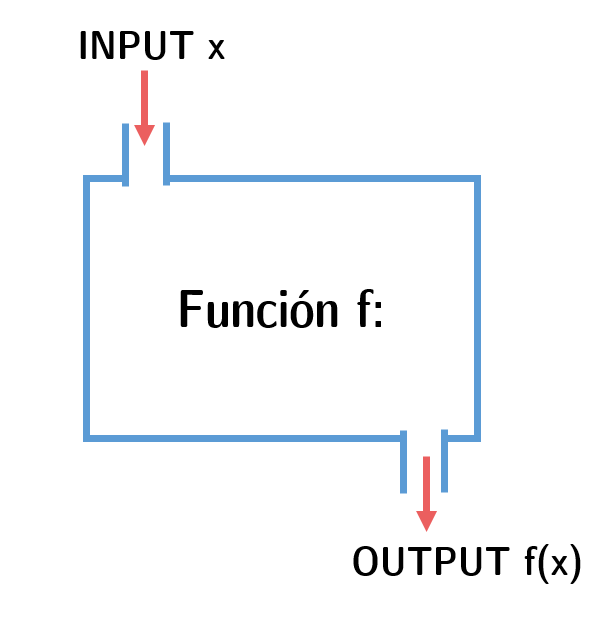
\includegraphics[width=8.54in]{00-images/rbas-funs} \end{center}

\texttt{sqrt()} toma un valor numérico como input y devuelve su raíz
cuadrada como output. \texttt{log()} toma el mismo input, pero devuelve
su logaritmo común (o en base a 10). \texttt{c()} toma distintos valores
únicos como input y devuelve un vector que los concatena.

Es a propósito de los vectores que las funciones de R comienzan a
brillar y a alejarse de las cualidades básicas de una calculadora (que,
a grandes rasgos, es lo que hemos visto ahora de R, nada muy
impresionante). Veamos algunas funciones que extraen información útil
sobre nuestro vector. ¿Qué hace cada una?

\begin{Shaded}
\begin{Highlighting}[]
\KeywordTok{mean}\NormalTok{(vector_}\DecValTok{1}\NormalTok{) }\CommentTok{# media}
\CommentTok{## [1] 15}
\KeywordTok{median}\NormalTok{(vector_}\DecValTok{1}\NormalTok{) }\CommentTok{# mediana}
\CommentTok{## [1] 15}
\KeywordTok{sd}\NormalTok{(vector_}\DecValTok{1}\NormalTok{) }\CommentTok{# desviación estándar}
\CommentTok{## [1] 5}
\KeywordTok{sum}\NormalTok{(vector_}\DecValTok{1}\NormalTok{) }\CommentTok{# suma}
\CommentTok{## [1] 45}
\KeywordTok{min}\NormalTok{(vector_}\DecValTok{1}\NormalTok{) }\CommentTok{# valor mínimo}
\CommentTok{## [1] 10}
\KeywordTok{max}\NormalTok{(vector_}\DecValTok{1}\NormalTok{) }\CommentTok{# valor máximo}
\CommentTok{## [1] 20}
\KeywordTok{length}\NormalTok{(vector_}\DecValTok{1}\NormalTok{) }\CommentTok{# longitud (cantidad de valores)}
\CommentTok{## [1] 3}
\KeywordTok{sort}\NormalTok{(vector_}\DecValTok{1}\NormalTok{) }\CommentTok{# ...}
\CommentTok{## [1] 10 15 20}
\end{Highlighting}
\end{Shaded}

El lector podría haber deducido que \texttt{sort()}, la última función
del lote anterior, ordena al vector de menor a mayor. ¿Qué pasa si
quisiéramos ordenarlo de mayor a menor? Esto nos permite introducir a
los \emph{argumentos}, partes de las funciones que nos permiten
modificar su comportamiento. A continuación agregaremos el argumento
\texttt{decreasing\ =\ TRUE} al comando anterior, consiguiendo nuestro
objetivo:

\begin{Shaded}
\begin{Highlighting}[]
\KeywordTok{sort}\NormalTok{(vector_}\DecValTok{1}\NormalTok{, }\DataTypeTok{decreasing =} \OtherTok{TRUE}\NormalTok{)}
\CommentTok{## [1] 20 15 10}
\end{Highlighting}
\end{Shaded}

\hypertarget{archivos-graficos-paquetes-ayuda}{%
\subsection{Archivos / gráficos / paquetes /
ayuda}\label{archivos-graficos-paquetes-ayuda}}

En el panel inferior derecho de RStudio estas cuatro pestañas son las
que se roban la película.

\hypertarget{archivos}{%
\subsubsection{Archivos}\label{archivos}}

Esta pestaña es una ventana a nuestros archivos. Funcionando como un
pequeño gestor, nos permite moverlos, renombrarlos, copiarlos, etcétera.
A propósito de archivos, una de las grandes novedades recientes de R son
los \emph{RStudio Projects}, o proyectos de RStudio. Los desarrolladores
de RStudio se dieron cuenta de que sus usuarios tenían scripts y otros
archivos de R (de los que aprenderemos luego, como bases de datos)
desperdigados a lo largo y ancho de sus discos duros, sin orden alguno.
Por eso implementaron la filosofía de ``un proyecto, una carpeta''. Es
tan simple como suena: la idea es que cada proyecto en el que trabajemos
sea autosuficiente, que incluya todo lo que necesitemos en una sola
carpeta. Se pueden manejar los proyectos desde la esquina superior
derecha de R. El lector debe ser cuidadoso y notar que crear o abrir un
proyecto reiniciará su sesión de R, borrando todo el trabajo que no
guarde.

\emph{(F: creo que podemos expandir un poquito mas en la utilidad de los
proyectos con un ejemplo, a mi me ha resultado muy grato el tema de los
proyectos!)}

\emph{(screenshot de RStudio Projects)}

\hypertarget{graficos}{%
\subsubsection{Gráficos}\label{graficos}}

Aquí aparecen los gráficos que realizamos con R. ¡En el capítulo
\emph{X} aprenderemos a crearlos!

\hypertarget{paquetes}{%
\subsubsection{Paquetes}\label{paquetes}}

Una de las cualidades de R a la que más hincapié hemos dado es su
versatilidad. Su código libre hace que muchos desarrolladores se sientan
atraídos a aportar a la comunidad de R con nuevas funcionalidades. En
general, realizan esto a través de paquetes, que los usuarios pueden
instalar como apéndices adicionales a R. Los paquetes contienen nuevas
funciones, bases de datos, etcétera. La pestaña de RStudio aquí reseñada
nos permite acceder a nuestros paquetes instalados.

Instalar un paquete es bastante simple, a través de la función
\texttt{install.packages()}. A continuación vamos a instalar el paquete
``tidyverse'', central en nuestros próximos análisis. El tidyverse es
una recopilación que incluye algunos de los mejores paquetes modernos
para análisis de datos en R.

\begin{Shaded}
\begin{Highlighting}[]
\KeywordTok{install.packages}\NormalTok{(}\StringTok{"tidyverse"}\NormalTok{)}
\end{Highlighting}
\end{Shaded}

Cada vez que el usuario abre una nueva sesión de R, este carga ``como de
fábrica''. No solo sin objetos, sino que solo con los paquetes básicos
que permiten a R funcionar. Tenemos que cargar los paquetes extra que
queramos usar, entonces. Es más o menos como cuando compramos un
\emph{smartphone} y descargamos las aplicaciones que más usaremos, para
que se ajuste a nuestras necesidades cotidianas. La forma más común de
hacer esto es a través de la función \texttt{library()}, como se ve a
continuación:

\begin{Shaded}
\begin{Highlighting}[]
\KeywordTok{library}\NormalTok{(}\StringTok{"tidyverse"}\NormalTok{)}
\end{Highlighting}
\end{Shaded}

El lector puede ahorrarse el trabajo de instalar los paquetes utilizados
en \emph{AnalizaR Datos Políticos} en el futuro y hacerlo todo ahora,
corriendo el siguiente súper comando. Ojo: ¡esto no lo salvará de cargar
los paquetes en cada nueva sesión de R que inicie! Ojo 2: puede que esto
le tome un tiempo considerable.

\emph{paquetes a instalar} \emph{F: excelente que vamos a ofrecer esto,
puede haber un paquete llamado ADP que tenga todo?}

\hypertarget{ayuda}{%
\subsubsection{Ayuda}\label{ayuda}}

Buscar ayuda es central a la hora de programar (y no solo de
programar\ldots{}). Esta pestaña de RStudio abre los archivos de ayuda
que necesitemos, permitiéndonos buscar en ellos. Las funciones tienen
archivos de ayuda para sí solas. Por ejemplo, podemos acceder al archivo
de ayuda de la función \texttt{sqrt()} a través del comando
\texttt{help(sqrt)}. Los paquetes en su conjunto también tienen archivos
de ayuda, más comprensivos. Por ejemplo, para ver los archivos de ayuda
del tidyverse solo debemos recurrir al argumento ``package'':
\texttt{help(package\ =\ tidyverse)}. El lector debe notar que los
archivos de ayuda de paquetes y funciones de paquetes solo están
disponibles si el paquete ha sido cargado.

\hypertarget{ejercicios}{%
\section{Ejercicios}\label{ejercicios}}

\begin{itemize}
\tightlist
\item
  ¿Qué significa ``correr'' un comando desde un script? ¿Cómo se hace?
\item
  ¿Cuál es la media de los dígitos del hit de Rafaella Carrà, 0 3 0 3 4
  5 6? ¿Y la mediana? Por último, órdenelos de mayor a menor.
\item
  Busque ayuda para el paquete ``googledrive''. Recomendado:
  maravillarse con la variedad de los paquetes de R.
\end{itemize}

\hypertarget{manejo}{%
\chapter{Manejo}\label{manejo}}

\textbf{F: EN GENERAL YO METERIA MAS SUB-SUBTITULOS, CASI UNO POR
FUNCION. POR EJ, UNO PARA ARRANGE (4.3.1), OTRO PARA SELECT
(4.4.1)\ldots{} O AL LADO DEL TITULO PONDRIA LA FUNCION: 4.4.
SELECCIONAR COLUMNAS CON }'SELECT'*****

Cuando hablamos de análisis de datos, casi siempre nos referimos a
análisis de \emph{bases de datos}. Aunque hay varios formatos de bases
de datos disponibles, en ciencias sociales generalmente usamos y creamos
\emph{bases de datos tabulares}, que son las que este libro tratará. Muy
probablemente el lector estará familiarizado con la estructura básica de
este tipo de bases, gracias a las planillas de Microsoft Excel, Google
Spreadsheets y/o LibreOffice Calc. La primera fila suele ser un
\textbf{header} o encabezado, que indica qué datos registran las celdas
de esa columna. En general, queremos que nuestras bases de datos
tabulares tengan una estructura \emph{tidy}, como la siguiente:

\begin{center}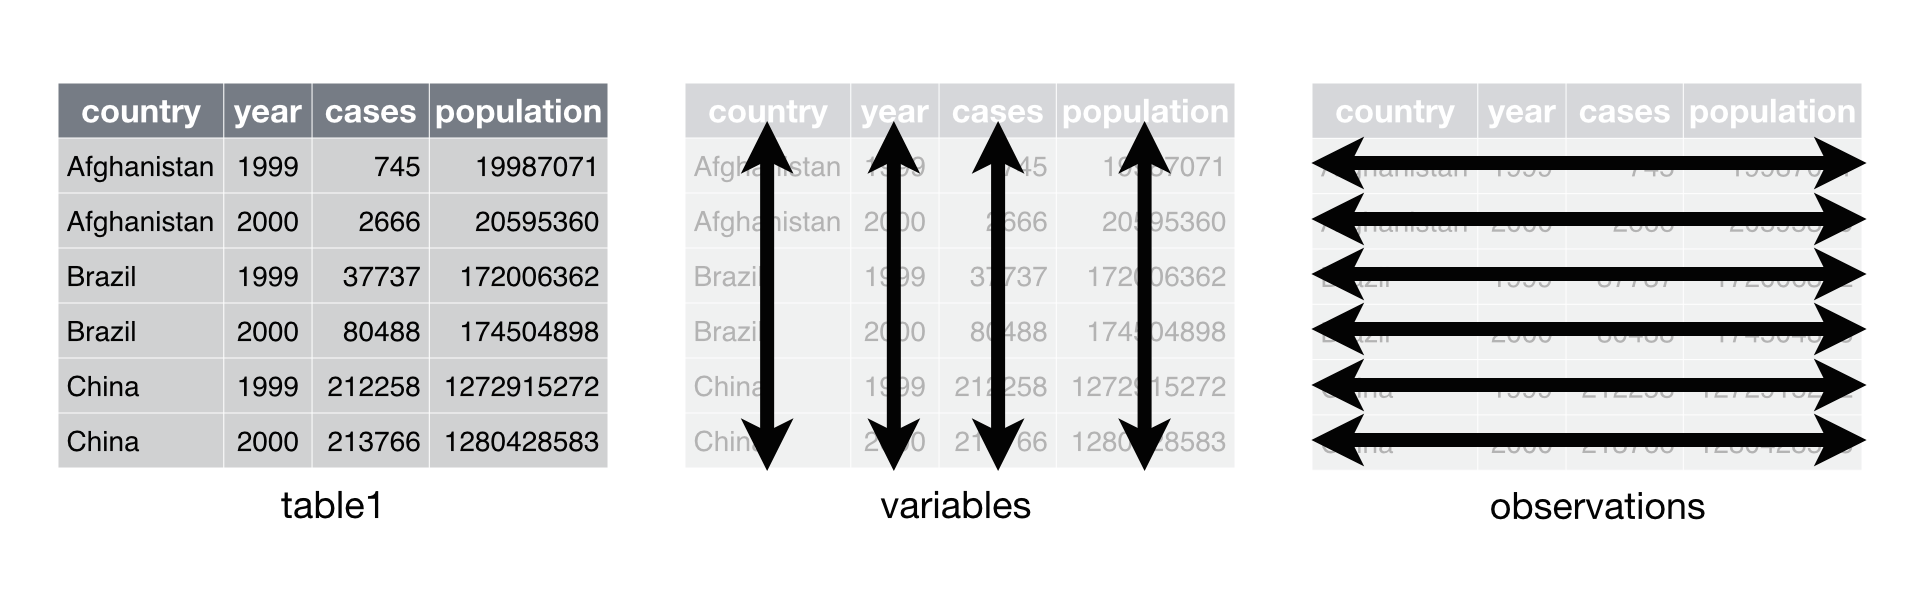
\includegraphics[width=0.6\linewidth]{00-images/manejo_tidy-4} \end{center}

La idea de una base \emph{tidy} es simple: cada columna es una variable,
cada fila una observación (de acuerdo a la unidad de análisis) y, por lo
tanto, cada celda es una observación. \emph{(explicar que este nombre lo
tomamos del dios Wickham y que es una idea tan simple que mucha gente no
la va a entender. Quien solo ha trabajado con Stata o Excel nunca vio
datos no-tidy)}

\hypertarget{nuestra-base-de-datos}{%
\section{Nuestra base de datos}\label{nuestra-base-de-datos}}

Para este capítulo usaremos una sección de la base de datos de
\emph{Quality of Government}(QoG,
2017){[}\url{https://qog.pol.gu.se}{]}, un proyecto que registra
diversos datos de países. Sus primeras observaciones son las siguientes:

\begin{tabular}{l|r|r|r|r|r|l}
\hline
cname & wdi\_gdppppcon2011 & wdi\_pop & ti\_cpi & lp\_muslim80 & fh\_ipolity2 & region\\
\hline
Afghanistan & 5.8e+10 & 3.1e+07 & 8 & 99.3 & 2.0 & Southern Asia\\
\hline
Albania & 2.9e+10 & 2.9e+06 & 31 & 20.5 & 8.1 & Southern Europe\\
\hline
Algeria & 5.1e+11 & 3.8e+07 & 36 & 99.1 & 4.2 & Northern Africa\\
\hline
Angola & 1.5e+11 & 2.3e+07 & 23 & 0.0 & 3.2 & Middle Africa\\
\hline
Australia & 9.9e+11 & 2.3e+07 & 81 & 0.2 & 10.0 & Australia and New Zealand\\
\hline
Austria & 3.7e+11 & 8.5e+06 & 69 & 0.6 & 10.0 & Western Europe\\
\hline
\end{tabular}

Las variables son las siguientes:

\begin{longtable}[]{@{}ll@{}}
\toprule
\begin{minipage}[b]{0.16\columnwidth}\raggedright
variable\strut
\end{minipage} & \begin{minipage}[b]{0.79\columnwidth}\raggedright
descripción\strut
\end{minipage}\tabularnewline
\midrule
\endhead
\begin{minipage}[t]{0.16\columnwidth}\raggedright
cname\strut
\end{minipage} & \begin{minipage}[t]{0.79\columnwidth}\raggedright
Nombre del país\strut
\end{minipage}\tabularnewline
\begin{minipage}[t]{0.16\columnwidth}\raggedright
wdi\_gdppppcon2011\strut
\end{minipage} & \begin{minipage}[t]{0.79\columnwidth}\raggedright
GDP PPP, en dólares del 2011, según los datos de WDI (p.~635 del
codebook)\strut
\end{minipage}\tabularnewline
\begin{minipage}[t]{0.16\columnwidth}\raggedright
wdi\_pop\strut
\end{minipage} & \begin{minipage}[t]{0.79\columnwidth}\raggedright
Población, según los datos de WDI (p.~665)\strut
\end{minipage}\tabularnewline
\begin{minipage}[t]{0.16\columnwidth}\raggedright
ti\_cpi\strut
\end{minipage} & \begin{minipage}[t]{0.79\columnwidth}\raggedright
Índice de Percepción de la Corrupción de TI. Va de 0 a 100, con 0 lo más
corrupto (p.~560)\strut
\end{minipage}\tabularnewline
\begin{minipage}[t]{0.16\columnwidth}\raggedright
lp\_muslim80\strut
\end{minipage} & \begin{minipage}[t]{0.79\columnwidth}\raggedright
Porcentaje de población de religión musulmana, para 1980, según LP
(p.~447)\strut
\end{minipage}\tabularnewline
\begin{minipage}[t]{0.16\columnwidth}\raggedright
fh\_ipolity2\strut
\end{minipage} & \begin{minipage}[t]{0.79\columnwidth}\raggedright
Nivel de democracia según FH. Va de 0 a 10, con 0 como menos democrático
(p.~291)\strut
\end{minipage}\tabularnewline
\begin{minipage}[t]{0.16\columnwidth}\raggedright
region\strut
\end{minipage} & \begin{minipage}[t]{0.79\columnwidth}\raggedright
Región del país, según WDI (añadida a la base)\strut
\end{minipage}\tabularnewline
\bottomrule
\end{longtable}

Para comenzar a trabajar carguemos el paquete \texttt{tidyverse}, uno de
los centrales del libro, que nos dará funciones útiles para trabajar con
nuestra base datos.

\begin{Shaded}
\begin{Highlighting}[]
\KeywordTok{library}\NormalTok{(tidyverse)}
\end{Highlighting}
\end{Shaded}

Ahora carguemos la base de datos a nuestro ambiente de trabajo en R.
Vamos a llamarla ``qog\_mod'' (QoG modificada). El archivo está en
formato .csv, por lo que utilizaremos la función del tidyverse
\texttt{read\_csv()}

\begin{Shaded}
\begin{Highlighting}[]
\NormalTok{qog_mod <-}\StringTok{ }\KeywordTok{read_csv}\NormalTok{(}\StringTok{"00-datos/manejo_04_qog_mod.csv"}\NormalTok{)}
\CommentTok{## Parsed with column specification:}
\CommentTok{## cols(}
\CommentTok{##   cname = col_character(),}
\CommentTok{##   wdi_gdppppcon2011 = col_double(),}
\CommentTok{##   wdi_pop = col_double(),}
\CommentTok{##   ti_cpi = col_double(),}
\CommentTok{##   lp_muslim80 = col_double(),}
\CommentTok{##   fh_ipolity2 = col_double(),}
\CommentTok{##   region = col_character()}
\CommentTok{## )}
\end{Highlighting}
\end{Shaded}

(hay que decidir cómo se va a hacer esto: desde carpeta local, url,
paquete, etc.) \emph{(F:opino que creemos un url del libro y usemos los
html, en el paquete ADP solo pondria funciones)}

\hypertarget{describir-la-base}{%
\section{Describir la base}\label{describir-la-base}}

(aquí podría ir \texttt{describe\_all()} u otra función de descripción
de la base, habría que decidir si esto tiene sentido en términos
pedagógicos; otra opción es hacer otro capítulo con
\texttt{group\_by()}, \texttt{tabyl()}, \texttt{crosstab()}, etc; me
inclino por esta última opción)

Para aproximarnos a nuestra base recién cargada tenemos varias opciones.
Podemos, como antes, simplemente usar su nombre como un comando para un
resumen rápido:

\begin{Shaded}
\begin{Highlighting}[]
\NormalTok{qog_mod}
\CommentTok{## # A tibble: 139 x 7}
\CommentTok{##    cname  wdi_gdppppcon20~ wdi_pop ti_cpi lp_muslim80 fh_ipolity2 region  }
\CommentTok{##    <chr>             <dbl>   <dbl>  <dbl>       <dbl>       <dbl> <chr>   }
\CommentTok{##  1 Afgha~      57566228480  3.07e7      8      99.3         2.02  Souther~}
\CommentTok{##  2 Alban~      28715335680  2.90e6     31      20.5         8.08  Souther~}
\CommentTok{##  3 Alger~     507901640704  3.82e7     36      99.1         4.25  Norther~}
\CommentTok{##  4 Angola     152477499392  2.34e7     23       0           3.25  Middle ~}
\CommentTok{##  5 Austr~     990474338304  2.31e7     81       0.200      10     Austral~}
\CommentTok{##  6 Austr~     373413642240  8.48e6     69       0.600      10     Western~}
\CommentTok{##  7 Baham~       8497731584  3.78e5     71       0          10     Caribbe~}
\CommentTok{##  8 Bahra~      56583507968  1.35e6     48      95           0.833 Western~}
\CommentTok{##  9 Bangl~     446835425280  1.57e8     27      85.9         6.42  Souther~}
\CommentTok{## 10 Barba~       4333428224  2.83e5     75       0.200      10     Caribbe~}
\CommentTok{## # ... with 129 more rows}
\end{Highlighting}
\end{Shaded}

También podemos utilizar la función \texttt{glimpse()} para tener un
resumen desde otra perspectiva:

\begin{Shaded}
\begin{Highlighting}[]
\KeywordTok{glimpse}\NormalTok{(qog_mod)}
\CommentTok{## Observations: 139}
\CommentTok{## Variables: 7}
\CommentTok{## $ cname             <chr> "Afghanistan", "Albania", "Algeria", "Angola...}
\CommentTok{## $ wdi_gdppppcon2011 <dbl> 5.8e+10, 2.9e+10, 5.1e+11, 1.5e+11, 9.9e+11,...}
\CommentTok{## $ wdi_pop           <dbl> 3.1e+07, 2.9e+06, 3.8e+07, 2.3e+07, 2.3e+07,...}
\CommentTok{## $ ti_cpi            <dbl> 8, 31, 36, 23, 81, 69, 71, 48, 27, 75, 75, 6...}
\CommentTok{## $ lp_muslim80       <dbl> 99.3, 20.5, 99.1, 0.0, 0.2, 0.6, 0.0, 95.0, ...}
\CommentTok{## $ fh_ipolity2       <dbl> 2.02, 8.08, 4.25, 3.25, 10.00, 10.00, 10.00,...}
\CommentTok{## $ region            <chr> "Southern Asia", "Southern Europe", "Norther...}
\end{Highlighting}
\end{Shaded}

Una alternativa que nos permite ver la base completa es la función
\texttt{View()}, análoga a clickear nuestro objeto en la pestaña
``Environment'' de Rstudio:

\begin{Shaded}
\begin{Highlighting}[]
\KeywordTok{View}\NormalTok{(qog_mod)}
\end{Highlighting}
\end{Shaded}

\hypertarget{ordenar-la-base-con-arrange}{%
\section{\texorpdfstring{Ordenar la base con
\texttt{arrange()}}{Ordenar la base con arrange()}}\label{ordenar-la-base-con-arrange}}

Una de las operaciones más comunes con bases de datos es ordenarlas de
acuerdo a alguna de las variables. Esto nos puede dar insights
(¿traducción?) inmediatos sobre nuestras observaciones. Por ejemplo,
ordenemos la base de acuerdo a población:

\begin{Shaded}
\begin{Highlighting}[]
\KeywordTok{arrange}\NormalTok{(qog_mod, wdi_pop)}
\CommentTok{## # A tibble: 139 x 7}
\CommentTok{##    cname   wdi_gdppppcon20~ wdi_pop ti_cpi lp_muslim80 fh_ipolity2 region }
\CommentTok{##    <chr>              <dbl>   <dbl>  <dbl>       <dbl>       <dbl> <chr>  }
\CommentTok{##  1 Domini~        722668736   72005   58         0           10    Caribb~}
\CommentTok{##  2 Seyche~       2229991168   89900   54         0.300        6.94 Easter~}
\CommentTok{##  3 Tonga          513904512  105139   31.4       0            8.59 Polyne~}
\CommentTok{##  4 Kiriba~        183852816  108544   30.8       0           10    Micron~}
\CommentTok{##  5 St Luc~       1871906688  182305   71         0           10    Caribb~}
\CommentTok{##  6 Sao To~        540452288  182386   42         0            8.59 Middle~}
\CommentTok{##  7 Samoa         1047012608  190390   52         0            8.59 Polyne~}
\CommentTok{##  8 Barbad~       4333428224  282503   75         0.200       10    Caribb~}
\CommentTok{##  9 Iceland      13266284544  323764   78         0           10    Northe~}
\CommentTok{## 10 Bahamas       8497731584  377841   71         0           10    Caribb~}
\CommentTok{## # ... with 129 more rows}
\end{Highlighting}
\end{Shaded}

El lector debe notar cómo el primer argumento, ``qog\_mod'', toma la
base de datos y los siguientes enuncian \textbf{cómo} ordenarla, en este
caso, por ``wdi\_pop'', la variable de población.

Debe notar también cómo el comando anterior no crea ningún objeto, solo
muestra los resultados en la consola. Para crear uno tenemos que seguir
la fórmula típica de asignación:

\begin{Shaded}
\begin{Highlighting}[]
\NormalTok{qog_mod_ordenada <-}\StringTok{ }\KeywordTok{arrange}\NormalTok{(qog_mod, wdi_pop)}
\end{Highlighting}
\end{Shaded}

Podemos realizar ambas operaciones, mostrar los resultados y crear el
objeto, rodeando este último comando con paréntesis:

\begin{Shaded}
\begin{Highlighting}[]
\NormalTok{( qog_mod_ordenada <-}\StringTok{ }\KeywordTok{arrange}\NormalTok{(qog_mod, wdi_pop) )}
\CommentTok{## # A tibble: 139 x 7}
\CommentTok{##    cname   wdi_gdppppcon20~ wdi_pop ti_cpi lp_muslim80 fh_ipolity2 region }
\CommentTok{##    <chr>              <dbl>   <dbl>  <dbl>       <dbl>       <dbl> <chr>  }
\CommentTok{##  1 Domini~        722668736   72005   58         0           10    Caribb~}
\CommentTok{##  2 Seyche~       2229991168   89900   54         0.300        6.94 Easter~}
\CommentTok{##  3 Tonga          513904512  105139   31.4       0            8.59 Polyne~}
\CommentTok{##  4 Kiriba~        183852816  108544   30.8       0           10    Micron~}
\CommentTok{##  5 St Luc~       1871906688  182305   71         0           10    Caribb~}
\CommentTok{##  6 Sao To~        540452288  182386   42         0            8.59 Middle~}
\CommentTok{##  7 Samoa         1047012608  190390   52         0            8.59 Polyne~}
\CommentTok{##  8 Barbad~       4333428224  282503   75         0.200       10    Caribb~}
\CommentTok{##  9 Iceland      13266284544  323764   78         0           10    Northe~}
\CommentTok{## 10 Bahamas       8497731584  377841   71         0           10    Caribb~}
\CommentTok{## # ... with 129 more rows}
\end{Highlighting}
\end{Shaded}

La operación para ordenar realizada antes iba de menor a mayor, en
términos de población. Si queremos el orden inverso (decreciente), basta
con añadir un signo menos (-) antes de la variable:

\begin{Shaded}
\begin{Highlighting}[]
\KeywordTok{arrange}\NormalTok{(qog_mod, }\OperatorTok{-}\NormalTok{wdi_pop)}
\CommentTok{## # A tibble: 139 x 7}
\CommentTok{##    cname   wdi_gdppppcon20~ wdi_pop ti_cpi lp_muslim80 fh_ipolity2 region }
\CommentTok{##    <chr>              <dbl>   <dbl>  <dbl>       <dbl>       <dbl> <chr>  }
\CommentTok{##  1 China     16023988207616  1.36e9     40       2.40         1.17 Easter~}
\CommentTok{##  2 India      6566166134784  1.28e9     36      11.6          8.5  Southe~}
\CommentTok{##  3 United~   16230494765056  3.16e8     73       0.800       10    Northe~}
\CommentTok{##  4 Indone~    2430921605120  2.51e8     32      43.4          7.83 South-~}
\CommentTok{##  5 Brazil     3109301780480  2.04e8     42       0.100        8.67 South ~}
\CommentTok{##  6 Pakist~     810954457088  1.81e8     28      96.8          6.33 Southe~}
\CommentTok{##  7 Nigeria     941462781952  1.73e8     25      45            5.58 Wester~}
\CommentTok{##  8 Bangla~     446835425280  1.57e8     27      85.9          6.42 Southe~}
\CommentTok{##  9 Japan      4535077044224  1.27e8     74       0           10    Easter~}
\CommentTok{## 10 Mexico     1997247479808  1.24e8     34       0            7.83 Centra~}
\CommentTok{## # ... with 129 more rows}
\end{Highlighting}
\end{Shaded}

¡Con eso tenemos los países con mayor población en el mundo! ¿Qué pasa
si queremos los países con mayor población \textbf{dentro de cada
región}? Tendríamos que realizar un ordenamiento en dos pasos: primero
por región y luego por población. Con \texttt{arrange()} esto es simple:

\begin{Shaded}
\begin{Highlighting}[]
\KeywordTok{arrange}\NormalTok{(qog_mod, region, }\OperatorTok{-}\NormalTok{wdi_pop)}
\CommentTok{## # A tibble: 139 x 7}
\CommentTok{##    cname   wdi_gdppppcon20~ wdi_pop ti_cpi lp_muslim80 fh_ipolity2 region }
\CommentTok{##    <chr>              <dbl>   <dbl>  <dbl>       <dbl>       <dbl> <chr>  }
\CommentTok{##  1 Austra~     990474338304  2.31e7     81       0.200       10    Austra~}
\CommentTok{##  2 New Ze~     148189986816  4.44e6     91       0           10    Austra~}
\CommentTok{##  3 Cuba        226685157376  1.14e7     46       0            1.17 Caribb~}
\CommentTok{##  4 Haiti        16999370752  1.04e7     19       0            4.58 Caribb~}
\CommentTok{##  5 Domini~     122657308672  1.03e7     29       0            8.25 Caribb~}
\CommentTok{##  6 Jamaica      22884503552  2.71e6     38       0.100        8.5  Caribb~}
\CommentTok{##  7 Trinid~      40973463552  1.35e6     38       6.5          9.17 Caribb~}
\CommentTok{##  8 Bahamas       8497731584  3.78e5     71       0           10    Caribb~}
\CommentTok{##  9 Barbad~       4333428224  2.83e5     75       0.200       10    Caribb~}
\CommentTok{## 10 St Luc~       1871906688  1.82e5     71       0           10    Caribb~}
\CommentTok{## # ... with 129 more rows}
\end{Highlighting}
\end{Shaded}

A propósito del resultado anterior, el lector puede deducir que cuando
\texttt{arrange()} ordena variables categóricas (en vez de numéricas) lo
hace alfabéticamente. Añadir un signo menos (-) antes de la variable
hará que el orden sea al revés en términos del alfabeto:

\begin{Shaded}
\begin{Highlighting}[]
\KeywordTok{arrange}\NormalTok{(qog_mod, }\KeywordTok{desc}\NormalTok{(region), }\OperatorTok{-}\NormalTok{wdi_pop) }\CommentTok{# no sé por qué - no funciona, ARREGLAR}
\CommentTok{## # A tibble: 139 x 7}
\CommentTok{##    cname   wdi_gdppppcon2011 wdi_pop ti_cpi lp_muslim80 fh_ipolity2 region}
\CommentTok{##    <chr>               <dbl>   <dbl>  <dbl>       <dbl>       <dbl> <chr> }
\CommentTok{##  1 France~     2459435270144  6.59e7     71       3            9.75 Weste~}
\CommentTok{##  2 Nether~      762382450688  1.68e7     83       1           10    Weste~}
\CommentTok{##  3 Belgium      452154359808  1.12e7     75       1.10         9.5  Weste~}
\CommentTok{##  4 Austria      373413642240  8.48e6     69       0.600       10    Weste~}
\CommentTok{##  5 Switze~      444201566208  8.09e6     85       0.300       10    Weste~}
\CommentTok{##  6 Luxemb~       48842280960  5.43e5     80       0           10    Weste~}
\CommentTok{##  7 Turkey      1392197369856  7.50e7     50      99.2          7.67 Weste~}
\CommentTok{##  8 Iraq         510895521792  3.38e7     16      95.8          4.5  Weste~}
\CommentTok{##  9 Saudi ~     1478747750400  3.02e7     46      98.8          0    Weste~}
\CommentTok{## 10 United~      560986259456  9.04e6     69      94.9          1.33 Weste~}
\CommentTok{## # ... with 129 more rows}
\end{Highlighting}
\end{Shaded}

\hypertarget{seleccionar-columnas-de-la-base-con-select}{%
\section{\texorpdfstring{Seleccionar columnas de la base con
\texttt{select()}}{Seleccionar columnas de la base con select()}}\label{seleccionar-columnas-de-la-base-con-select}}

A veces queremos trabajar solo con algunas variables de una base de
datos. Para esto existe la función \texttt{select()}. Pensemos que
queremos solo el nombre de cada país (cname) y su porcentaje de
población musulmana para 1980:

\begin{Shaded}
\begin{Highlighting}[]
\KeywordTok{select}\NormalTok{(qog_mod, cname, lp_muslim80)}
\CommentTok{## # A tibble: 139 x 2}
\CommentTok{##    cname       lp_muslim80}
\CommentTok{##    <chr>             <dbl>}
\CommentTok{##  1 Afghanistan      99.3  }
\CommentTok{##  2 Albania          20.5  }
\CommentTok{##  3 Algeria          99.1  }
\CommentTok{##  4 Angola            0    }
\CommentTok{##  5 Australia         0.200}
\CommentTok{##  6 Austria           0.600}
\CommentTok{##  7 Bahamas           0    }
\CommentTok{##  8 Bahrain          95    }
\CommentTok{##  9 Bangladesh       85.9  }
\CommentTok{## 10 Barbados          0.200}
\CommentTok{## # ... with 129 more rows}
\end{Highlighting}
\end{Shaded}

Al igual que para \texttt{arrange()}, aquí el primer argumento designa
la base a modificar y los demás cómo se debería hacer eso -en este caso,
qué variables deben ser seleccionadas.

Añadir un signo menos (-) aquí indica qué variables \emph{no}
seleccionar. Por ejemplo, quitemos el porcentaje de población musulmana
para 1980 de la base:

\begin{Shaded}
\begin{Highlighting}[]
\KeywordTok{select}\NormalTok{(qog_mod, }\OperatorTok{-}\NormalTok{lp_muslim80)}
\CommentTok{## # A tibble: 139 x 6}
\CommentTok{##    cname     wdi_gdppppcon20~  wdi_pop ti_cpi fh_ipolity2 region          }
\CommentTok{##    <chr>                <dbl>    <dbl>  <dbl>       <dbl> <chr>           }
\CommentTok{##  1 Afghanis~      57566228480   3.07e7      8       2.02  Southern Asia   }
\CommentTok{##  2 Albania        28715335680   2.90e6     31       8.08  Southern Europe }
\CommentTok{##  3 Algeria       507901640704   3.82e7     36       4.25  Northern Africa }
\CommentTok{##  4 Angola        152477499392   2.34e7     23       3.25  Middle Africa   }
\CommentTok{##  5 Australia     990474338304   2.31e7     81      10     Australia and N~}
\CommentTok{##  6 Austria       373413642240   8.48e6     69      10     Western Europe  }
\CommentTok{##  7 Bahamas         8497731584   3.78e5     71      10     Caribbean       }
\CommentTok{##  8 Bahrain        56583507968   1.35e6     48       0.833 Western Asia    }
\CommentTok{##  9 Banglade~     446835425280   1.57e8     27       6.42  Southern Asia   }
\CommentTok{## 10 Barbados        4333428224   2.83e5     75      10     Caribbean       }
\CommentTok{## # ... with 129 more rows}
\end{Highlighting}
\end{Shaded}

Aparte de seleccionar variables específicas, \texttt{select()} es capaz
de entender referencias a intervalos de variables. Por ejemplo, podemos
querer las cuatro primeras variables:

\begin{Shaded}
\begin{Highlighting}[]
\KeywordTok{select}\NormalTok{(qog_mod, cname}\OperatorTok{:}\NormalTok{ti_cpi)}
\CommentTok{## # A tibble: 139 x 4}
\CommentTok{##    cname       wdi_gdppppcon2011   wdi_pop ti_cpi}
\CommentTok{##    <chr>                   <dbl>     <dbl>  <dbl>}
\CommentTok{##  1 Afghanistan       57566228480  30682500      8}
\CommentTok{##  2 Albania           28715335680   2897366     31}
\CommentTok{##  3 Algeria          507901640704  38186136     36}
\CommentTok{##  4 Angola           152477499392  23448202     23}
\CommentTok{##  5 Australia        990474338304  23125868     81}
\CommentTok{##  6 Austria          373413642240   8479375     69}
\CommentTok{##  7 Bahamas            8497731584    377841     71}
\CommentTok{##  8 Bahrain           56583507968   1349427     48}
\CommentTok{##  9 Bangladesh       446835425280 157157392     27}
\CommentTok{## 10 Barbados           4333428224    282503     75}
\CommentTok{## # ... with 129 more rows}
\KeywordTok{select}\NormalTok{(qog_mod, }\DecValTok{1}\OperatorTok{:}\DecValTok{4}\NormalTok{) }\CommentTok{# lo mismo, aunque no recomendado}
\CommentTok{## # A tibble: 139 x 4}
\CommentTok{##    cname       wdi_gdppppcon2011   wdi_pop ti_cpi}
\CommentTok{##    <chr>                   <dbl>     <dbl>  <dbl>}
\CommentTok{##  1 Afghanistan       57566228480  30682500      8}
\CommentTok{##  2 Albania           28715335680   2897366     31}
\CommentTok{##  3 Algeria          507901640704  38186136     36}
\CommentTok{##  4 Angola           152477499392  23448202     23}
\CommentTok{##  5 Australia        990474338304  23125868     81}
\CommentTok{##  6 Austria          373413642240   8479375     69}
\CommentTok{##  7 Bahamas            8497731584    377841     71}
\CommentTok{##  8 Bahrain           56583507968   1349427     48}
\CommentTok{##  9 Bangladesh       446835425280 157157392     27}
\CommentTok{## 10 Barbados           4333428224    282503     75}
\CommentTok{## # ... with 129 more rows}
\end{Highlighting}
\end{Shaded}

Otra herramienta para complejizar nuestra selección se encuentra en las
funciones de ayuda. Entre ellas, \texttt{starts\_with} es de particular
utilidad, permitiendo seleccionar variables que empiecen con cierto
patrón. Por ejemplo, podríamos querer, a partir del nombre del país,
todas las variables que provengan de los World Development Indicators
(WDI) del Banco Mundial:

\begin{Shaded}
\begin{Highlighting}[]
\KeywordTok{select}\NormalTok{(qog_mod, cname, }\KeywordTok{starts_with}\NormalTok{(}\StringTok{"wdi_"}\NormalTok{))}
\CommentTok{## # A tibble: 139 x 3}
\CommentTok{##    cname       wdi_gdppppcon2011   wdi_pop}
\CommentTok{##    <chr>                   <dbl>     <dbl>}
\CommentTok{##  1 Afghanistan       57566228480  30682500}
\CommentTok{##  2 Albania           28715335680   2897366}
\CommentTok{##  3 Algeria          507901640704  38186136}
\CommentTok{##  4 Angola           152477499392  23448202}
\CommentTok{##  5 Australia        990474338304  23125868}
\CommentTok{##  6 Austria          373413642240   8479375}
\CommentTok{##  7 Bahamas            8497731584    377841}
\CommentTok{##  8 Bahrain           56583507968   1349427}
\CommentTok{##  9 Bangladesh       446835425280 157157392}
\CommentTok{## 10 Barbados           4333428224    282503}
\CommentTok{## # ... with 129 more rows}
\end{Highlighting}
\end{Shaded}

Otra función de ayuda útil es \texttt{everything()}, que se lee como
``todas las demás variables''. Es especialmente útil para cambiar el
orden de las variables en una bases de datos. Por ejemplo, pasemos
región al segundo lugar entre las variables:

\begin{Shaded}
\begin{Highlighting}[]
\KeywordTok{select}\NormalTok{(qog_mod, cname, region, }\KeywordTok{everything}\NormalTok{())}
\CommentTok{## # A tibble: 139 x 7}
\CommentTok{##    cname  region   wdi_gdppppcon20~ wdi_pop ti_cpi lp_muslim80 fh_ipolity2}
\CommentTok{##    <chr>  <chr>               <dbl>   <dbl>  <dbl>       <dbl>       <dbl>}
\CommentTok{##  1 Afgha~ Souther~      57566228480  3.07e7      8      99.3         2.02 }
\CommentTok{##  2 Alban~ Souther~      28715335680  2.90e6     31      20.5         8.08 }
\CommentTok{##  3 Alger~ Norther~     507901640704  3.82e7     36      99.1         4.25 }
\CommentTok{##  4 Angola Middle ~     152477499392  2.34e7     23       0           3.25 }
\CommentTok{##  5 Austr~ Austral~     990474338304  2.31e7     81       0.200      10    }
\CommentTok{##  6 Austr~ Western~     373413642240  8.48e6     69       0.600      10    }
\CommentTok{##  7 Baham~ Caribbe~       8497731584  3.78e5     71       0          10    }
\CommentTok{##  8 Bahra~ Western~      56583507968  1.35e6     48      95           0.833}
\CommentTok{##  9 Bangl~ Souther~     446835425280  1.57e8     27      85.9         6.42 }
\CommentTok{## 10 Barba~ Caribbe~       4333428224  2.83e5     75       0.200      10    }
\CommentTok{## # ... with 129 more rows}
\end{Highlighting}
\end{Shaded}

\hypertarget{renombrar-columnas-de-la-base-con-rename}{%
\section{\texorpdfstring{Renombrar columnas de la base con
\texttt{rename()}}{Renombrar columnas de la base con rename()}}\label{renombrar-columnas-de-la-base-con-rename}}

La notación para el GDP es un poco confusa. ¿Y si queremos cambiar el
nombre de la variable? Aprovechemos también de cambiar el nombre de la
variable de identificación por país.

\begin{Shaded}
\begin{Highlighting}[]
\KeywordTok{rename}\NormalTok{(qog_mod, }\DataTypeTok{wdi_gdp =}\NormalTok{ wdi_gdppppcon2011, }\DataTypeTok{country_name =}\NormalTok{ cname)}
\CommentTok{## # A tibble: 139 x 7}
\CommentTok{##    country_name  wdi_gdp  wdi_pop ti_cpi lp_muslim80 fh_ipolity2 region   }
\CommentTok{##    <chr>           <dbl>    <dbl>  <dbl>       <dbl>       <dbl> <chr>    }
\CommentTok{##  1 Afghanistan   5.76e10   3.07e7      8      99.3         2.02  Southern~}
\CommentTok{##  2 Albania       2.87e10   2.90e6     31      20.5         8.08  Southern~}
\CommentTok{##  3 Algeria       5.08e11   3.82e7     36      99.1         4.25  Northern~}
\CommentTok{##  4 Angola        1.52e11   2.34e7     23       0           3.25  Middle A~}
\CommentTok{##  5 Australia     9.90e11   2.31e7     81       0.200      10     Australi~}
\CommentTok{##  6 Austria       3.73e11   8.48e6     69       0.600      10     Western ~}
\CommentTok{##  7 Bahamas       8.50e 9   3.78e5     71       0          10     Caribbean}
\CommentTok{##  8 Bahrain       5.66e10   1.35e6     48      95           0.833 Western ~}
\CommentTok{##  9 Bangladesh    4.47e11   1.57e8     27      85.9         6.42  Southern~}
\CommentTok{## 10 Barbados      4.33e 9   2.83e5     75       0.200      10     Caribbean}
\CommentTok{## # ... with 129 more rows}
\end{Highlighting}
\end{Shaded}

\hypertarget{filtrar-observaciones-de-la-base-con-filter}{%
\section{\texorpdfstring{Filtrar observaciones de la base con
\texttt{filter()}}{Filtrar observaciones de la base con filter()}}\label{filtrar-observaciones-de-la-base-con-filter}}

Es muy común el querer filtrar nuestras observaciones de acuerdo a algún
tipo de criterio lógico. Para esto R cuenta con operadores lógicos. Los
más comunes son los siguientes:

\begin{longtable}[]{@{}cl@{}}
\toprule
operador & descripción\tabularnewline
\midrule
\endhead
== & es igual a\tabularnewline
!= & es distinto a\tabularnewline
\textgreater{} & es mayor a\tabularnewline
\textless{} & es menor a\tabularnewline
\textgreater{}= & es mayor o igual a\tabularnewline
\textless{}= & es menor o igual a\tabularnewline
\& & y (intersección)\tabularnewline
&\tabularnewline
\bottomrule
\end{longtable}

Por ejemplo, podríamos querer solo los países (observaciones)
sudamericanos. Hacer esto con \texttt{filter()} es simple, con la ayuda
de operadores lógicos:

\begin{Shaded}
\begin{Highlighting}[]
\KeywordTok{filter}\NormalTok{(qog_mod, region }\OperatorTok{==}\StringTok{ "South America"}\NormalTok{)}
\CommentTok{## # A tibble: 11 x 7}
\CommentTok{##    cname  wdi_gdppppcon2011 wdi_pop ti_cpi lp_muslim80 fh_ipolity2 region }
\CommentTok{##    <chr>              <dbl>   <dbl>  <dbl>       <dbl>       <dbl> <chr>  }
\CommentTok{##  1 Boliv~       63344840704  1.04e7     34       0            7.58 South ~}
\CommentTok{##  2 Brazil     3109301780480  2.04e8     42       0.100        8.67 South ~}
\CommentTok{##  3 Chile       383162515456  1.76e7     71       0           10    South ~}
\CommentTok{##  4 Colom~      582488686592  4.73e7     36       0.200        7.17 South ~}
\CommentTok{##  5 Ecuad~      166412222464  1.57e7     35       0            7.08 South ~}
\CommentTok{##  6 Guyana        5066298368  7.61e5     27       9            7.75 South ~}
\CommentTok{##  7 Parag~       53195030528  6.47e6     24       0            8.08 South ~}
\CommentTok{##  8 Peru        346126876672  3.06e7     38       0            8.5  South ~}
\CommentTok{##  9 Surin~        8388805120  5.33e5     36      13            7.92 South ~}
\CommentTok{## 10 Urugu~       65827684352  3.41e6     73       0           10    South ~}
\CommentTok{## 11 Venez~      535572054016  3.03e7     20       0            5.17 South ~}
\end{Highlighting}
\end{Shaded}

¿Qué pasa si queremos solo las filas de países sudamericanos con más de
10 millones de habitantes (nos quedamos con 8 de 12)?

¿Cuáles son los filtros que aplican los siguientes comandos?

\begin{Shaded}
\begin{Highlighting}[]
\KeywordTok{filter}\NormalTok{(qog_mod, fh_ipolity2 }\OperatorTok{>}\StringTok{ }\DecValTok{9}\NormalTok{)}
\CommentTok{## # A tibble: 39 x 7}
\CommentTok{##    cname  wdi_gdppppcon2011 wdi_pop ti_cpi lp_muslim80 fh_ipolity2 region }
\CommentTok{##    <chr>              <dbl>   <dbl>  <dbl>       <dbl>       <dbl> <chr>  }
\CommentTok{##  1 Austr~      990474338304  2.31e7     81       0.200        10   Austra~}
\CommentTok{##  2 Austr~      373413642240  8.48e6     69       0.600        10   Wester~}
\CommentTok{##  3 Baham~        8497731584  3.78e5     71       0            10   Caribb~}
\CommentTok{##  4 Barba~        4333428224  2.83e5     75       0.200        10   Caribb~}
\CommentTok{##  5 Belgi~      452154359808  1.12e7     75       1.10          9.5 Wester~}
\CommentTok{##  6 Canada     1484141756416  3.52e7     81       0.600        10   Northe~}
\CommentTok{##  7 Cape ~        3109324800  5.07e5     58       0            10   Wester~}
\CommentTok{##  8 Chile       383162515456  1.76e7     71       0            10   South ~}
\CommentTok{##  9 Costa~       65419849728  4.71e6     53       0            10   Centra~}
\CommentTok{## 10 Cypru~       25927987200  1.14e6     63      18.5          10   Wester~}
\CommentTok{## # ... with 29 more rows}

\KeywordTok{filter}\NormalTok{(qog_mod, wdi_pop }\OperatorTok{>}\StringTok{ }\FloatTok{10e7}\NormalTok{)}
\CommentTok{## # A tibble: 10 x 7}
\CommentTok{##    cname   wdi_gdppppcon20~ wdi_pop ti_cpi lp_muslim80 fh_ipolity2 region }
\CommentTok{##    <chr>              <dbl>   <dbl>  <dbl>       <dbl>       <dbl> <chr>  }
\CommentTok{##  1 Bangla~     446835425280  1.57e8     27      85.9          6.42 Southe~}
\CommentTok{##  2 Brazil     3109301780480  2.04e8     42       0.100        8.67 South ~}
\CommentTok{##  3 China     16023988207616  1.36e9     40       2.40         1.17 Easter~}
\CommentTok{##  4 India      6566166134784  1.28e9     36      11.6          8.5  Southe~}
\CommentTok{##  5 Indone~    2430921605120  2.51e8     32      43.4          7.83 South-~}
\CommentTok{##  6 Japan      4535077044224  1.27e8     74       0           10    Easter~}
\CommentTok{##  7 Mexico     1997247479808  1.24e8     34       0            7.83 Centra~}
\CommentTok{##  8 Nigeria     941462781952  1.73e8     25      45            5.58 Wester~}
\CommentTok{##  9 Pakist~     810954457088  1.81e8     28      96.8          6.33 Southe~}
\CommentTok{## 10 United~   16230494765056  3.16e8     73       0.800       10    Northe~}

\KeywordTok{filter}\NormalTok{(qog_mod, cname }\OperatorTok{!=}\StringTok{ "Albania"}\NormalTok{)}
\CommentTok{## # A tibble: 138 x 7}
\CommentTok{##    cname  wdi_gdppppcon20~ wdi_pop ti_cpi lp_muslim80 fh_ipolity2 region  }
\CommentTok{##    <chr>             <dbl>   <dbl>  <dbl>       <dbl>       <dbl> <chr>   }
\CommentTok{##  1 Afgha~      57566228480  3.07e7      8      99.3         2.02  Souther~}
\CommentTok{##  2 Alger~     507901640704  3.82e7     36      99.1         4.25  Norther~}
\CommentTok{##  3 Angola     152477499392  2.34e7     23       0           3.25  Middle ~}
\CommentTok{##  4 Austr~     990474338304  2.31e7     81       0.200      10     Austral~}
\CommentTok{##  5 Austr~     373413642240  8.48e6     69       0.600      10     Western~}
\CommentTok{##  6 Baham~       8497731584  3.78e5     71       0          10     Caribbe~}
\CommentTok{##  7 Bahra~      56583507968  1.35e6     48      95           0.833 Western~}
\CommentTok{##  8 Bangl~     446835425280  1.57e8     27      85.9         6.42  Souther~}
\CommentTok{##  9 Barba~       4333428224  2.83e5     75       0.200      10     Caribbe~}
\CommentTok{## 10 Belgi~     452154359808  1.12e7     75       1.10        9.5   Western~}
\CommentTok{## # ... with 128 more rows}

\KeywordTok{filter}\NormalTok{(qog_mod, lp_muslim80 }\OperatorTok{>=}\StringTok{ }\DecValTok{95}\NormalTok{)}
\CommentTok{## # A tibble: 15 x 7}
\CommentTok{##    cname   wdi_gdppppcon20~ wdi_pop ti_cpi lp_muslim80 fh_ipolity2 region }
\CommentTok{##    <chr>              <dbl>   <dbl>  <dbl>       <dbl>       <dbl> <chr>  }
\CommentTok{##  1 Afghan~      57566228480  3.07e7    8          99.3       2.02  Southe~}
\CommentTok{##  2 Algeria     507901640704  3.82e7   36          99.1       4.25  Northe~}
\CommentTok{##  3 Bahrain      56583507968  1.35e6   48          95         0.833 Wester~}
\CommentTok{##  4 Iran       1236225490944  7.72e7   25          97.9       1.58  Southe~}
\CommentTok{##  5 Iraq        510895521792  3.38e7   16          95.8       4.5   Wester~}
\CommentTok{##  6 Kuwait      266584637440  3.59e6   43          95.1       2.42  Wester~}
\CommentTok{##  7 Libya       122544226304  6.27e6   15          98.1       4.58  Northe~}
\CommentTok{##  8 Maldiv~       4501654016  3.93e5   24.7        99.9       5.30  Southe~}
\CommentTok{##  9 Maurit~      13920699392  3.87e6   30          99.4       3.25  Wester~}
\CommentTok{## 10 Morocco     240604184576  3.35e7   37          99.4       3.58  Northe~}
\CommentTok{## 11 Oman        151726620672  3.91e6   47          98.9       1.75  Wester~}
\CommentTok{## 12 Pakist~     810954457088  1.81e8   28          96.8       6.33  Southe~}
\CommentTok{## 13 Saudi ~    1478747750400  3.02e7   46          98.8       0     Wester~}
\CommentTok{## 14 Tunisia     116821843968  1.09e7   41          99.4       7.33  Northe~}
\CommentTok{## 15 Turkey     1392197369856  7.50e7   50          99.2       7.67  Wester~}

\KeywordTok{filter}\NormalTok{(qog_mod, region }\OperatorTok{==}\StringTok{ "South America"} \OperatorTok{&}\StringTok{ }\NormalTok{wdi_pop }\OperatorTok{>}\StringTok{ }\FloatTok{10e6}\NormalTok{)}
\CommentTok{## # A tibble: 7 x 7}
\CommentTok{##   cname   wdi_gdppppcon20~ wdi_pop ti_cpi lp_muslim80 fh_ipolity2 region  }
\CommentTok{##   <chr>              <dbl>   <dbl>  <dbl>       <dbl>       <dbl> <chr>   }
\CommentTok{## 1 Bolivia      63344840704  1.04e7     34       0            7.58 South A~}
\CommentTok{## 2 Brazil     3109301780480  2.04e8     42       0.100        8.67 South A~}
\CommentTok{## 3 Chile       383162515456  1.76e7     71       0           10    South A~}
\CommentTok{## 4 Colomb~     582488686592  4.73e7     36       0.200        7.17 South A~}
\CommentTok{## 5 Ecuador     166412222464  1.57e7     35       0            7.08 South A~}
\CommentTok{## 6 Peru        346126876672  3.06e7     38       0            8.5  South A~}
\CommentTok{## 7 Venezu~     535572054016  3.03e7     20       0            5.17 South A~}

\KeywordTok{filter}\NormalTok{(qog_mod, region }\OperatorTok{==}\StringTok{ "South America"} \OperatorTok{|}\StringTok{ }\NormalTok{region }\OperatorTok{==}\StringTok{ "South-Eastern Asia"}\NormalTok{)}
\CommentTok{## # A tibble: 19 x 7}
\CommentTok{##    cname   wdi_gdppppcon20~ wdi_pop ti_cpi lp_muslim80 fh_ipolity2 region }
\CommentTok{##    <chr>              <dbl>   <dbl>  <dbl>       <dbl>       <dbl> <chr>  }
\CommentTok{##  1 Bolivia      63344840704  1.04e7     34       0            7.58 South ~}
\CommentTok{##  2 Brazil     3109301780480  2.04e8     42       0.100        8.67 South ~}
\CommentTok{##  3 Cambod~      44559769600  1.51e7     20       2.40         4.25 South-~}
\CommentTok{##  4 Chile       383162515456  1.76e7     71       0           10    South ~}
\CommentTok{##  5 Colomb~     582488686592  4.73e7     36       0.200        7.17 South ~}
\CommentTok{##  6 Ecuador     166412222464  1.57e7     35       0            7.08 South ~}
\CommentTok{##  7 Guyana        5066298368  7.61e5     27       9            7.75 South ~}
\CommentTok{##  8 Indone~    2430921605120  2.51e8     32      43.4          7.83 South-~}
\CommentTok{##  9 Laos         31582838784  6.58e6     26       1            1.17 South-~}
\CommentTok{## 10 Malays~     690044600320  2.95e7     50      49.4          6.5  South-~}
\CommentTok{## 11 Paragu~      53195030528  6.47e6     24       0            8.08 South ~}
\CommentTok{## 12 Peru        346126876672  3.06e7     38       0            8.5  South ~}
\CommentTok{## 13 Philip~     621044039680  9.76e7     36       4.30         7.83 South-~}
\CommentTok{## 14 Singap~     419630612480  5.40e6     86      17.4          4.5  South-~}
\CommentTok{## 15 Vietnam     459724881920  8.97e7     31       1            1.58 South-~}
\CommentTok{## 16 Surina~       8388805120  5.33e5     36      13            7.92 South ~}
\CommentTok{## 17 Thaila~    1007950299136  6.75e7     35       3.90         6.75 South-~}
\CommentTok{## 18 Uruguay      65827684352  3.41e6     73       0           10    South ~}
\CommentTok{## 19 Venezu~     535572054016  3.03e7     20       0            5.17 South ~}
\end{Highlighting}
\end{Shaded}

\hypertarget{crear-nuevas-variables-en-la-base-con-mutate}{%
\section{\texorpdfstring{Crear nuevas variables en la base con
\texttt{mutate()}}{Crear nuevas variables en la base con mutate()}}\label{crear-nuevas-variables-en-la-base-con-mutate}}

Muchas veces queremos crear nuevas variables, a partir de las que ya
tenemos. Por ejemplo, podríamos querer el GDP per capita, en vez del
absoluto. Tenemos los ingredientes para calcularlo: el GDP absoluto y la
población. Creemos una nueva variable, entonces:

\begin{Shaded}
\begin{Highlighting}[]
\KeywordTok{mutate}\NormalTok{(qog_mod, }\DataTypeTok{gdp_ppp_per_capita =}\NormalTok{ wdi_gdppppcon2011}\OperatorTok{/}\NormalTok{wdi_pop)}
\CommentTok{## # A tibble: 139 x 8}
\CommentTok{##    cname wdi_gdppppcon20~ wdi_pop ti_cpi lp_muslim80 fh_ipolity2 region}
\CommentTok{##    <chr>            <dbl>   <dbl>  <dbl>       <dbl>       <dbl> <chr> }
\CommentTok{##  1 Afgh~      57566228480  3.07e7      8      99.3         2.02  South~}
\CommentTok{##  2 Alba~      28715335680  2.90e6     31      20.5         8.08  South~}
\CommentTok{##  3 Alge~     507901640704  3.82e7     36      99.1         4.25  North~}
\CommentTok{##  4 Ango~     152477499392  2.34e7     23       0           3.25  Middl~}
\CommentTok{##  5 Aust~     990474338304  2.31e7     81       0.200      10     Austr~}
\CommentTok{##  6 Aust~     373413642240  8.48e6     69       0.600      10     Weste~}
\CommentTok{##  7 Baha~       8497731584  3.78e5     71       0          10     Carib~}
\CommentTok{##  8 Bahr~      56583507968  1.35e6     48      95           0.833 Weste~}
\CommentTok{##  9 Bang~     446835425280  1.57e8     27      85.9         6.42  South~}
\CommentTok{## 10 Barb~       4333428224  2.83e5     75       0.200      10     Carib~}
\CommentTok{## # ... with 129 more rows, and 1 more variable: gdp_ppp_per_capita <dbl>}
\end{Highlighting}
\end{Shaded}

Otra nueva variable que podría interesarnos es el número de musulmanes
por país. Con la proporción de musulmanes y la población total del país
podemos hacer una buena estimación:

\begin{Shaded}
\begin{Highlighting}[]
\KeywordTok{mutate}\NormalTok{(qog_mod, }\DataTypeTok{n_muslim =}\NormalTok{ wdi_pop }\OperatorTok{*}\StringTok{ }\NormalTok{lp_muslim80)}
\CommentTok{## # A tibble: 139 x 8}
\CommentTok{##    cname wdi_gdppppcon20~ wdi_pop ti_cpi lp_muslim80 fh_ipolity2 region}
\CommentTok{##    <chr>            <dbl>   <dbl>  <dbl>       <dbl>       <dbl> <chr> }
\CommentTok{##  1 Afgh~      57566228480  3.07e7      8      99.3         2.02  South~}
\CommentTok{##  2 Alba~      28715335680  2.90e6     31      20.5         8.08  South~}
\CommentTok{##  3 Alge~     507901640704  3.82e7     36      99.1         4.25  North~}
\CommentTok{##  4 Ango~     152477499392  2.34e7     23       0           3.25  Middl~}
\CommentTok{##  5 Aust~     990474338304  2.31e7     81       0.200      10     Austr~}
\CommentTok{##  6 Aust~     373413642240  8.48e6     69       0.600      10     Weste~}
\CommentTok{##  7 Baha~       8497731584  3.78e5     71       0          10     Carib~}
\CommentTok{##  8 Bahr~      56583507968  1.35e6     48      95           0.833 Weste~}
\CommentTok{##  9 Bang~     446835425280  1.57e8     27      85.9         6.42  South~}
\CommentTok{## 10 Barb~       4333428224  2.83e5     75       0.200      10     Carib~}
\CommentTok{## # ... with 129 more rows, and 1 more variable: n_muslim <dbl>}
\end{Highlighting}
\end{Shaded}

¡Es posible crear más de una variable con el mismo comando! Creemos las
dos de antes, a la vez:

\begin{Shaded}
\begin{Highlighting}[]
\KeywordTok{mutate}\NormalTok{(qog_mod, }
       \DataTypeTok{gdp_ppp_per_capita =}\NormalTok{ wdi_gdppppcon2011}\OperatorTok{/}\NormalTok{wdi_pop,}
       \DataTypeTok{n_muslim           =}\NormalTok{ wdi_pop }\OperatorTok{*}\StringTok{ }\NormalTok{lp_muslim80)}
\CommentTok{## # A tibble: 139 x 9}
\CommentTok{##    cname wdi_gdppppcon20~ wdi_pop ti_cpi lp_muslim80 fh_ipolity2 region}
\CommentTok{##    <chr>            <dbl>   <dbl>  <dbl>       <dbl>       <dbl> <chr> }
\CommentTok{##  1 Afgh~      57566228480  3.07e7      8      99.3         2.02  South~}
\CommentTok{##  2 Alba~      28715335680  2.90e6     31      20.5         8.08  South~}
\CommentTok{##  3 Alge~     507901640704  3.82e7     36      99.1         4.25  North~}
\CommentTok{##  4 Ango~     152477499392  2.34e7     23       0           3.25  Middl~}
\CommentTok{##  5 Aust~     990474338304  2.31e7     81       0.200      10     Austr~}
\CommentTok{##  6 Aust~     373413642240  8.48e6     69       0.600      10     Weste~}
\CommentTok{##  7 Baha~       8497731584  3.78e5     71       0          10     Carib~}
\CommentTok{##  8 Bahr~      56583507968  1.35e6     48      95           0.833 Weste~}
\CommentTok{##  9 Bang~     446835425280  1.57e8     27      85.9         6.42  South~}
\CommentTok{## 10 Barb~       4333428224  2.83e5     75       0.200      10     Carib~}
\CommentTok{## # ... with 129 more rows, and 2 more variables: gdp_ppp_per_capita <dbl>,}
\CommentTok{## #   n_muslim <dbl>}
\end{Highlighting}
\end{Shaded}

\hypertarget{concatenar-comandos-las-pipes}{%
\section{\texorpdfstring{Concatenar comandos: las pipes
(\texttt{\%\textgreater{}\%})}{Concatenar comandos: las pipes (\%\textgreater{}\%)}}\label{concatenar-comandos-las-pipes}}

A menudo no queremos hacer una sola de las operaciones con bases de
datos reseñadas antes, sino que una seguidilla de estas. Si quisiéramos
crear una nueva base a través de, por ejemplo, (1) seleccionar las
variables de país, población y GDP, (2) crear la variable de GDP per
capita, y (3) ordenar los países de mayor a menor según GDP per capita,
nuestro procedimiento en R sería algo como esto:

\begin{Shaded}
\begin{Highlighting}[]
\NormalTok{qog_mod_seguidilla_}\DecValTok{1}\NormalTok{ <-}\StringTok{ }\KeywordTok{select}\NormalTok{(qog_mod, cname, wdi_pop, wdi_gdppppcon2011)}
\NormalTok{qog_mod_seguidilla_}\DecValTok{2}\NormalTok{ <-}\StringTok{ }\KeywordTok{mutate}\NormalTok{(qog_mod_seguidilla_}\DecValTok{1}\NormalTok{, }
                               \DataTypeTok{gdp_ppp_per_capita =}\NormalTok{ wdi_gdppppcon2011}\OperatorTok{/}\NormalTok{wdi_pop)}
\NormalTok{qog_mod_seguidilla_}\DecValTok{3}\NormalTok{ <-}\StringTok{ }\KeywordTok{arrange}\NormalTok{(qog_mod_seguidilla_}\DecValTok{2}\NormalTok{, }\OperatorTok{-}\NormalTok{gdp_ppp_per_capita)}
\end{Highlighting}
\end{Shaded}

\begin{Shaded}
\begin{Highlighting}[]
\NormalTok{qog_mod_seguidilla_}\DecValTok{3}
\CommentTok{## # A tibble: 139 x 4}
\CommentTok{##    cname                  wdi_pop wdi_gdppppcon2011 gdp_ppp_per_capita}
\CommentTok{##    <chr>                    <dbl>             <dbl>              <dbl>}
\CommentTok{##  1 Qatar                  2101288      280302059520            133395.}
\CommentTok{##  2 Luxembourg              543360       48842280960             89889.}
\CommentTok{##  3 Singapore              5399200      419630612480             77721.}
\CommentTok{##  4 Kuwait                 3593689      266584637440             74181.}
\CommentTok{##  5 Norway                 5079623      321651408896             63322.}
\CommentTok{##  6 United Arab Emirates   9039978      560986259456             62056.}
\CommentTok{##  7 Switzerland            8089346      444201566208             54912.}
\CommentTok{##  8 United States        316497536    16230494765056             51282.}
\CommentTok{##  9 Saudi Arabia          30201052     1478747750400             48963.}
\CommentTok{## 10 Ireland                4598294      212357021696             46182.}
\CommentTok{## # ... with 129 more rows}
\end{Highlighting}
\end{Shaded}

El lector notará que esto es bastante complicado y nos deja con dos
\textbf{objetos intermedios} que no nos interesan,
``qog\_mod\_seguidilla\_1'' y ``qog\_mod\_seguidilla\_2''.

La solución del paquete tidyverse que estamos utilizando son \textbf{las
pipes}. El lector notará que en las tres funciones de nuestra seguidilla
anterior (select, mutate y arrange) el primer argumento es la base de
datos a tratar. En vez de crear objetos intermedios podemos ``chutear''
la base de datos a través de nuestros comandos con pipes, omitiendo los
primeros argumentos:

\begin{Shaded}
\begin{Highlighting}[]
\NormalTok{qog_mod_seguidilla <-}\StringTok{ }\NormalTok{qog_mod }\OperatorTok
\StringTok{  }\KeywordTok{select}\NormalTok{(cname, wdi_pop, wdi_gdppppcon2011) }\OperatorTok
\StringTok{  }\KeywordTok{mutate}\NormalTok{(}\DataTypeTok{gdp_ppp_per_capita =}\NormalTok{ wdi_gdppppcon2011}\OperatorTok{/}\NormalTok{wdi_pop) }\OperatorTok
\StringTok{  }\KeywordTok{arrange}\NormalTok{(}\OperatorTok{-}\NormalTok{gdp_ppp_per_capita)}
\end{Highlighting}
\end{Shaded}

\begin{Shaded}
\begin{Highlighting}[]
\NormalTok{qog_mod_seguidilla}
\CommentTok{## # A tibble: 139 x 4}
\CommentTok{##    cname                  wdi_pop wdi_gdppppcon2011 gdp_ppp_per_capita}
\CommentTok{##    <chr>                    <dbl>             <dbl>              <dbl>}
\CommentTok{##  1 Qatar                  2101288      280302059520            133395.}
\CommentTok{##  2 Luxembourg              543360       48842280960             89889.}
\CommentTok{##  3 Singapore              5399200      419630612480             77721.}
\CommentTok{##  4 Kuwait                 3593689      266584637440             74181.}
\CommentTok{##  5 Norway                 5079623      321651408896             63322.}
\CommentTok{##  6 United Arab Emirates   9039978      560986259456             62056.}
\CommentTok{##  7 Switzerland            8089346      444201566208             54912.}
\CommentTok{##  8 United States        316497536    16230494765056             51282.}
\CommentTok{##  9 Saudi Arabia          30201052     1478747750400             48963.}
\CommentTok{## 10 Ireland                4598294      212357021696             46182.}
\CommentTok{## # ... with 129 more rows}
\end{Highlighting}
\end{Shaded}

Las pipes pueden leerse como ``pero luego''. Nuestra seguidilla
anterior, entonces, se leería de la siguiente forma:

\begin{quote}
qog\_mod\_seguilla es igual a qog\_mod; pero luego seleccionamos las
variables cname, wdi\_pop, wdi\_gdppppcon2011; pero luego creamos la
variable gdp\_ppp\_per\_capita; pero luego ordenamos la base en forma
decreciente según gdp\_ppp\_per\_capita.
\end{quote}

\hypertarget{ejercicios-1}{%
\section{Ejercicios}\label{ejercicios-1}}

\begin{itemize}
\tightlist
\item
  Cree una base nueva, llamada qog\_mod\_2, con una nueva variable
  llamada ``porc\_muslim'', que sea el porcentaje de población musulmana
  del país.
\item
  Cree una base nueva, llamada qog\_mod\_3, que incluya solo países
  latinoamericanos, China y Sudáfrica.
\item
  Cree una base nueva, llamada qog\_mod\_4, que incluya solo países con
  población mayor a la media de población entre todos los países. Debe
  contener solo las variables de nombre del país, región y población (en
  ese orden). Ordene la base según población, de mayor a menor. ¡Use
  pipes!
\end{itemize}

\hypertarget{dataviz}{%
\chapter{Visualización de datos}\label{dataviz}}

Por Soledad Araya

\hypertarget{por-que-quiero-visualizar-mis-datos}{%
\section{¿Por qué quiero visualizar mis
datos?}\label{por-que-quiero-visualizar-mis-datos}}

Ya aprendiste a manejar comandos del \texttt{tidyverse} y tienes ganas
de, rápidamente, sumergirte en el mundo de los gráficos y aplicar el
conocimiento adquirido en tu propia base de datos. Con el
\texttt{tidyverse} y \texttt{ggplot2} el manejo de datos en R se
simplifica de una manera impresionante, pero hay pasos anteriores que
debes realizar antes de empezar a escribir tu código. Por ejemplo,
conocer tus variables. Son variables continuas o categóricas, si es
categórica tiene dos o más niveles, y si esos niveles están ordenados o
no. Y esas no son las únicas preguntas. Parece muy simple, pero si no
tienes considerado esto previo a tu trabajo con \texttt{ggplot2} las
cosas se pueden poner feas muy rápido. Ejemplos de esto hay en
\href{https://twitter.com/accidental__aRt}{accidental aRt}.

Pregunta rápida: ¿por qué representamos gráficamente nuestros datos?

Primero, sé que muchos de nosotros tenemos un sentido estético demasiado
fuerte y queremos expresarlo de otras maneras. Las tablas no tienen la
capacidad de mostrar todo como lo quisiéramos. Pero tener buen o mal
gusto no significará una real diferencia si nuestros datos están malos,
si no sabemos graficar lo que tenemos en mente o si simplemente no
entendemos cómo funciona nuestro cerebro. No, no son clases de
neurociencia, pero sí tenemos que entender que la percepción es clave
cuando hablamos de visualización de datos. Insisto,
\href{https://twitter.com/accidental__aRt}{accidental aRt} es la muestra
de esto.

Pero, volvamos a la pregunta central: ¿por qué visualizar? ¿por qué no
simplemente hacer tablas que expresen lo que queremos decir? A través de
la visualización podemos entender otro tipo de problemáticas que los
números por sí solos no nos muestran. Al visualizar, queremos explorar y
entender nuestros datos. Con estos pasos previos, además ganamos la
capacidad de explicar qué pasa con ellos. Si no creen esta aproximación
a buenas primeras, hay muchos ejemplos que lo demuestran como el
cuarteto de
\href{http://www.sjsu.edu/faculty/gerstman/StatPrimer/anscombe1973.pdf}{Anscombe
(1973)}. Básicamente, los números por sí solos nos pueden decir, por
ejemplo, que existe una correlación entre dos variables, pero no nos
dirá la forma funcional de esa correlación.

\begin{figure}

{\centering 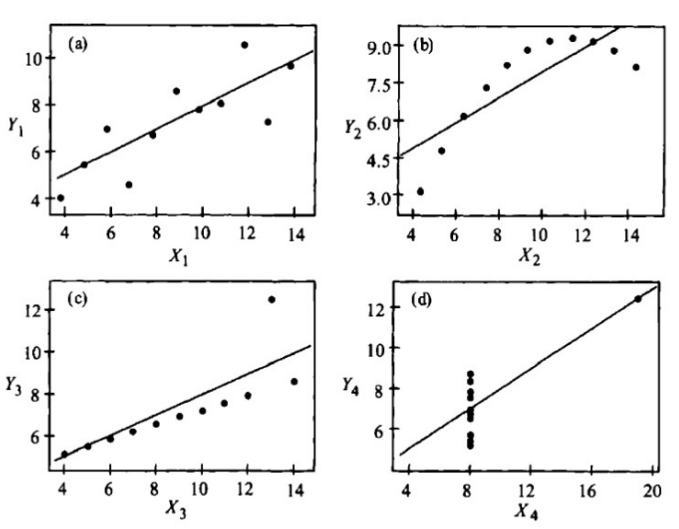
\includegraphics[width=1\linewidth]{00-images/dataviz_anscombe} 

}

\caption{Cuarteto de Anscombe.}\label{fig:anscombe}
\end{figure}

\href{https://link.springer.com/chapter/10.1007\%2F978-3-319-23446-5_3}{James
E. Monogan III, (2015)} ya resumía de forma muy simple, y para
cientistas sociales, por qué la visualización de datos es importante al
momento de trabajar con datos cuantitativos. En la introducción del
capítulo, Monogan en simples líneas nos habla de la importancia y la
ventaja que conlleva trabajar con imágenes, desde la simple distribución
de las variables, sus ouliers o sesgos; hasta el cambio de ellas a
través del tiempo. Por esta razón, la visualización de datos es una
herramienta fundamental para cualquiera que trabaje con datos. No es,
por ningún motivo, un ``movimiento estético''; graficar es
extremadamente útil.

Aun así, para algunos, la visualización de datos es tanto un elemento
funcional al análisis como un elemento estético por excelencia. Para
\href{http://pages.mtu.edu/~hcking/Tufte_hKing.pdf}{Edward R. Tufte,
(2006)} visualizar datos de forma efectiva tiene un componente artístico
inevitable. Con formación de estadista y Doctor en Ciencia Política de
la Universidad de Yale, Edward Tufte se dedicó a entender y explicar
sobre cómo la ciencia y el arte tienen en común \emph{la observación a
ojos abiertos que genera información empírica}. Su libro
\href{https://www.amazon.com/gp/product/0961392177/102-6444562-7552168?}{Beautiful
Evidence} describe el proceso de cómo \emph{ver} se transforma en
\emph{mostrar}, y cómo observación empírica se transforma en
explicaciones y evidencia.

\begin{figure}

{\centering 
\includegraphics[width=1\linewidth]{00-images/dataviz_beautiful_evidence} 

}

\caption{Portada de 'Beautiful Evidence'.}\label{fig:beautiful-evidence}
\end{figure}

Tenemos que entender que la visualización de datos es un lenguaje como
cualquier otro. Como emisores, tenemos que conocer a nuestra audiencia:
quiénes son los receptores del mensaje, si es un público experto o
simplemente gente de a pié. En cualquier circunstancia, nosotros
adecuaríamos nuestro mensaje al tipo de receptor. Cuando visualizamos es
lo mismo. Los gráficos que hacemos tienen que adecuarse a nuestro
público. Pero incluso con la gente más entendida no hay que abusar: no
se trata de aplicar todo lo que sabemos a la vez, sino de entender qué
estamos tratando de proyectar. Por lo tanto el código --entendido como
los signos y reglas-- tiene que tener un sentido e insertarse en un
contexto específico. Entender las funciones del lenguaje es fundamental.

Tanto el código como el canal tienen que ser adecuados para que todos
entiendan lo que estoy intentando mostrar con mis datos. Por eso, vale
preguntarse:

\begin{enumerate}
\def\labelenumi{\arabic{enumi}.}
\tightlist
\item
  ¿Mis datos están siendo bien \emph{representados}? ¿Escogí el tipo de
  gráfico \emph{adecuado} para mis datos?
\item
  Este tipo de representación ¿es \emph{efectiva}? ¿Estoy
  \emph{comunicando} lo que quiero comunicar?
\item
  Los elementos visuales ¿se \emph{entienden}? ¿Se \emph{leen} de forma
  correcta?
\end{enumerate}

El buen uso de las funciones del lenguaje no sólo sirven para rendir y
aprobar exámenes escritos. Sino también para entender que el mensaje no
se construye sólo con código. Hay mucho más detrás de eso.

En el siguiente ítem, hablaremos del funcionamiento de \texttt{ggplot2}
para entender un poco más cómo funciona. De ahí en adelante, empezaremos
con lo práctico. Para empezar, los tipos más comunes de representaciones
visuales como lo son el histograma, el gráfico de barras, de densidad,
de línea, entre otros. Además, introduciremos otros paquetes de
utilidades para hacer gráficos más sofisticados. Finalmente, veremos
algunos otros paquetes que nos pueden ser útiles dentro de las ciencias
sociales, y la ciencia política en particular, como lo son \texttt{sf} y
\texttt{ggparliament}.

Si quieres aprender más sobre visualización de datos, revisa
\href{http://socviz.co}{Data Visualization: A Practical introduction} de
Kieran Healy, un libro disponible de forma gratuita, que es entretenido
y didáctico para enseñar \texttt{ggplot2} paso a paso. En este libro no
sólo encontrarás la parte teórica, sino también la práctica. Por otro
lado, la página \href{https://www.data-to-viz.com/}{From Data to Viz}
puede hacerte de ayuda para saber cómo quieres presentar tus datos, pero
no sólo eso: ya sea que trabajes con R o Python, puedes encontrar los
paquetes y códigos para su aplicación.

\hypertarget{primeros-pasos}{%
\section{Primeros pasos}\label{primeros-pasos}}

Ahora que entendemos el proceso previo a la construcción del gráfico,
tenemos que familiarizarnos con \texttt{ggplot2}.
\href{https://byrneslab.net/classes/biol607/readings/wickham_layered-grammar.pdf}{A
Layered Grammar of Graphics} de Hadley Wickham, explica de forma
detallada el funcionamiento de esta nueva ``gramática'' para hacer
gráficos. Si dominas inglés, te recomiendo que leas de primera fuente
cómo se pensó este paquete y cómo entender el uso de las capas en la
construcción de los gráficos.

A pesar de que el uso de \texttt{ggplot2} se expandió rápidamente,
dentro de la comunidad de R hay constantes discusiones sobre la
enseñanza de \texttt{ggplot2} como primera opción, por sobre los
gráficos de R base. Por ejemplo,
\href{http://varianceexplained.org/r/why-I-use-ggplot2/}{David Robinson}
en su blog tiene diferentes entradas sobre este tema, donde él expone de
forma contundente las ventajas de \texttt{ggplot2} por sobre las otras
opciones. Si recién estás empezando a familiarizarte con R, empezar con
\texttt{ggplo2} te brindará herramientas muy poderosas y la curva de
aprendizaje no es tan elevada como lo requeriría R base.

Algunas de las ventajas que menciona David Robinson en ``Why I use
ggplot2'' son:

\begin{itemize}
\tightlist
\item
  ¡Leyendas! R base requiere de más conocimientos de los usuarios para
  poder hacer leyendas en los gráficos. Nuestro amigo \texttt{ggplot2}
  las hace automáticamente.
\item
  ¡Faceting! Suena extrañísimo, pero no encontré una traducción que le
  hiciera justicia. Básicamente, podemos crear subgráficos con terceras
  o cuartas variables que nos permita entender mejor el comportamiento
  de nuestros datos.
\item
  Trabaja en conjunto con el \texttt{tidyverse}. Eso quiere decir que
  podemos hacer más por menos. Al final del capítulo entenderán a lo que
  me refiero. Hay atajos para todo.
\item
  Estéticamente, es mejor. Ni hablar de las miles de opciones de paletas
  cromáticas, temas, fuentes, etc. Si no te gusta, existe una forma de
  cambiarlo.
\end{itemize}

Teniendo esto en consideración, comencemos con lo práctico.

\hypertarget{las-capas-del-multiverso-ggplotidiano}{%
\subsection{Las capas del multiverso
ggplotidiano}\label{las-capas-del-multiverso-ggplotidiano}}

Pero, entremos al tema que nos interesa: ¿Cómo funciona
\texttt{ggplot2}? Este paquete viene incluido en el \texttt{tidyverse},
por lo que no es necesario cargarlo de forma separada. Además, usaremos
las herramientas de ambos paquetes durante todo el capítulo. Cargamos el
paquete:

\begin{Shaded}
\begin{Highlighting}[]
\KeywordTok{library}\NormalTok{(tidyverse)}
\end{Highlighting}
\end{Shaded}

La intuición detrás de\texttt{ggplot2} es muy simple. La construcción de
los datos se hace en base a capas que contienen cierto tipo de
información.

\hypertarget{datos}{%
\subsubsection{Datos}\label{datos}}

La primera capa son los datos que utilizaremos. Para hacer esto un poco
más demostrativo, cargaremos los datos que usaremos a través de todo el
capítulo.

\begin{Shaded}
\begin{Highlighting}[]
\NormalTok{datos_municipales <-}\StringTok{ }\KeywordTok{read_rds}\NormalTok{(}\StringTok{"00-datos/dataviz_data_municipal_v3.rds"}\NormalTok{)}
\end{Highlighting}
\end{Shaded}

Estos datos corresponden a información sobre las municipalidades
chilenas. Algunos son del \href{http://www.servel.cl}{Servicio
Electoral} y otros del
\href{http://datos.sinim.gov.cl/datos_municipales.php}{Sistema Nacional
de Información Municipal} de Chile. En la primera, encontramos los
resultados de las elecciones locales, regionales y nacionales del país;
y en la segunda, encontramos características económicas, sociales y
demográficas de los municipios chilenos. En este caso, contamos con los
datos electorales comunales desde 1992 al 2012, y datos descriptivos
como la población, los ingresos totales de la municipalidad, el gasto en
asistencia social y el porcentaje de personas en situación de pobreza
según el total comunal de la Encuesta de Caracterización Socioeconómica
Nacional, CASEN.

\begin{Shaded}
\begin{Highlighting}[]
\KeywordTok{str}\NormalTok{(datos_municipales)}
\CommentTok{## Classes 'tbl_df', 'tbl' and 'data.frame':    1742 obs. of  6 variables:}
\CommentTok{##  $ year    : Factor w/ 6 levels "1992","1996",..: 1 1 1 1 1 1 1 1 1 1 ...}
\CommentTok{##  $ zona    : Factor w/ 5 levels "Norte Chico",..: 2 3 3 3 3 3 3 3 3 3 ...}
\CommentTok{##  $ comuna  : chr  "Iquique" "Dalcahue" "Fresia" "Futaleufu" ...}
\CommentTok{##  $ genero  : Factor w/ 2 levels "0","1": 1 1 1 1 1 1 1 1 1 1 ...}
\CommentTok{##  $ ingresos: int  NA NA NA NA NA NA NA NA NA NA ...}
\CommentTok{##  $ casen   : num  NA NA NA NA NA NA NA NA NA NA ...}
\end{Highlighting}
\end{Shaded}

Al mirar la base, encontramos que hay datos continuos (numéricos) y
categóricos (factores). Saber qué tipo de variable manejamos es base
para el siguiente paso.

\hypertarget{estetica}{%
\subsubsection{Estética}\label{estetica}}

La segunda capa corresponde al mapeo de las variables dentro del
espacio. En este paso, utilizamos \texttt{mapping\ =\ aes()}, el cual
contendrá la variable que tendremos en nuestro eje x y nuestro eje y.
Para \texttt{aes()} hay muchas más opciones que iremos viendo dentro del
capítulo, algunas de ellas son \texttt{fill}, \texttt{color},
\texttt{shape}, y \texttt{alpha}. Todas estas opciones son un conjunto
de signos que nos permitirán traducir de mejor manera lo que queremos
decir a través de nuestro gráfico. Normalmente, a estas opciones se le
llaman \emph{aesthetics} o \texttt{aes()}.

\begin{Shaded}
\begin{Highlighting}[]
\KeywordTok{ggplot}\NormalTok{(}\DataTypeTok{data    =}\NormalTok{ datos_municipales, }
       \DataTypeTok{mapping =} \KeywordTok{aes}\NormalTok{(}\DataTypeTok{x =}\NormalTok{ year, }\DataTypeTok{y =}\NormalTok{ casen))}
\end{Highlighting}
\end{Shaded}

\begin{center}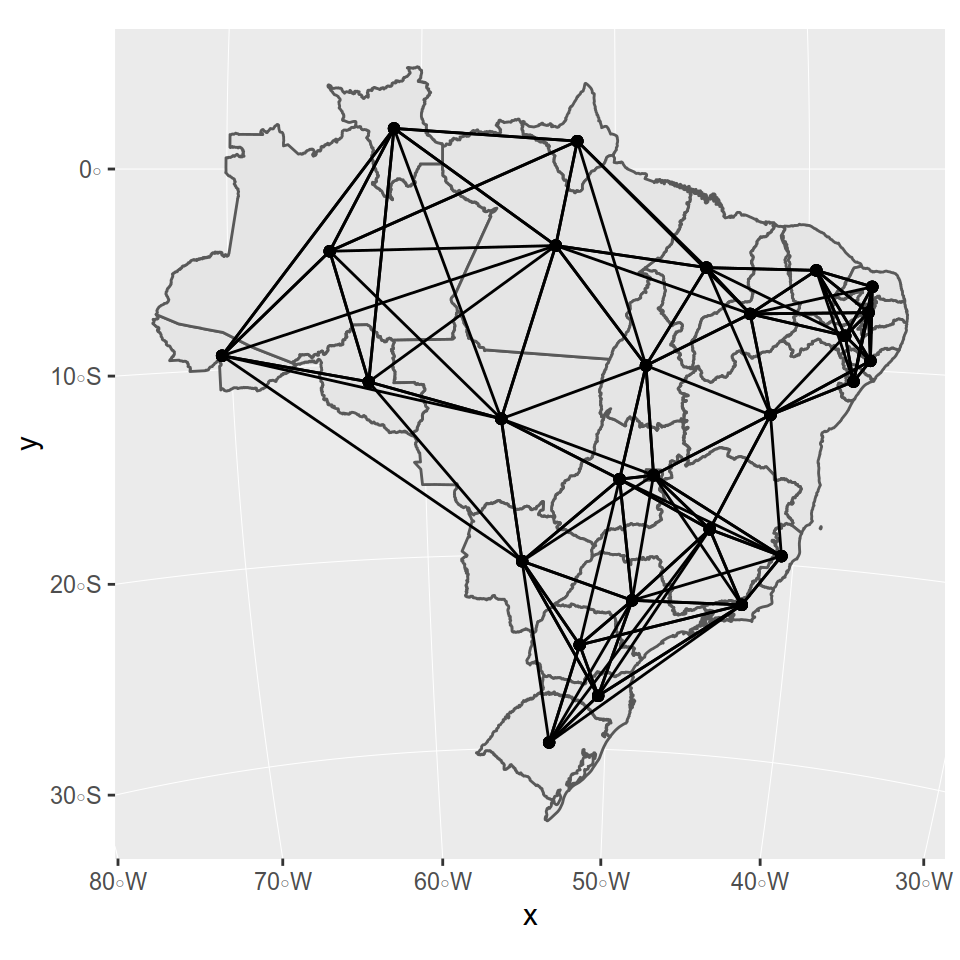
\includegraphics{adp-bookdown_files/figure-latex/unnamed-chunk-54-1} \end{center}

El resultado muestra un cuadro vacío. Eso es porque no lo hemos dicho
qué objeto geométrico es el que usaremos.

\hypertarget{objeto-geometrico}{%
\subsubsection{Objeto geométrico}\label{objeto-geometrico}}

Suena extraño, pero cuando hablamos de objeto geométrico o
\texttt{geom}, estamos hablando del tipo de gráfico que queremos hacer,
si un gráfico de línea, uno de barra, un histograma o un gráfico de
densidad, o de puntos, o si queremos hacer un boxplot. Esta es la
tercera capa. En este caso, como tenemos los datos de la encuesta CASEN,
haremos un boxplot para ver cómo se distribuyen los municipios de
nuestra muestra.

\begin{Shaded}
\begin{Highlighting}[]
\KeywordTok{ggplot}\NormalTok{(}\DataTypeTok{data    =}\NormalTok{ datos_municipales, }
       \DataTypeTok{mapping =} \KeywordTok{aes}\NormalTok{(}\DataTypeTok{x =}\NormalTok{ year, }\DataTypeTok{y =}\NormalTok{ casen)) }\OperatorTok{+}
\StringTok{  }\KeywordTok{geom_boxplot}\NormalTok{()}
\end{Highlighting}
\end{Shaded}

\begin{center}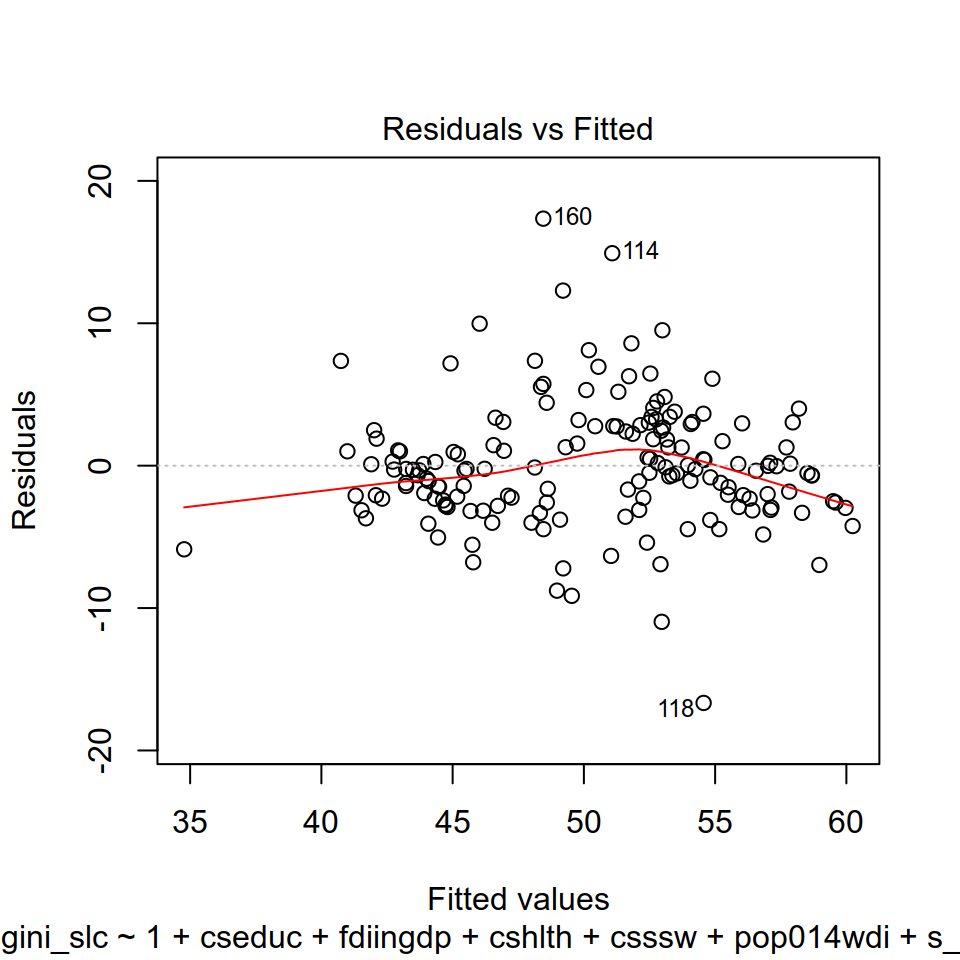
\includegraphics{adp-bookdown_files/figure-latex/unnamed-chunk-55-1} \end{center}

Lo primero que notamos es la ausencia de datos para tres periodos.
Lamentablemente, en el SINIM no hay datos anteriores al 2002, por eso no
hay registros para esos años. Por ese motivo, parece una buena idea
filtrar y dejar solo los años que tengan datos sobre la encuesta CASEN.
Además de eso, nuestro gráfico no nos dice mucho sobre el porcentaje de
pobreza y su distribución. Considerando la geografía chilena, sería una
buena idea que vieramos la distribución por zona.

\hypertarget{faceting}{%
\subsubsection{Faceting}\label{faceting}}

Ahora ocuparemos nuestras habilidades para hacer dos cosas: primero,
ocuparemos \texttt{filter} para dejar sólo los años que nos interesan.
Segundo, dividiremos los resultados por zona usando
\texttt{facet\_wrap}, la que corresponde a la cuarta capa que podemos
usar para armar un gráfico con \texttt{ggplot}. No siempre es necesaria,
pero siempre es útil mostrar lo que puede lograr. Cuando utilizamos esta
capa, lo que buscamos es organizar las geometrías que estamos utilizando
a través de una variable categórica. En este caso, zona. Pero el
\emph{faceting} como acción es mucho más que esto. \texttt{facet\_wrap}
y \texttt{facet\_grid} pueden tomar una serie de argumentos, donde el
primero es el más importante. La sintaxis que usamos en este caso es la
usada para fórmulas en R, y denotamos el primer argumento con el signo
``\textasciitilde{}''. Con \texttt{nrow} y \texttt{ncol} podemos
especificar cómo queremos ordenar nuestro gráfico.

Finalmente, agregamos dos líneas de código, una para filtrar y otra para
subdividir nuestra información. Esto es lo que logramos:

\begin{Shaded}
\begin{Highlighting}[]
\KeywordTok{ggplot}\NormalTok{(}\DataTypeTok{data    =}\NormalTok{ datos_municipales }\OperatorTok\StringTok{ }\KeywordTok{filter}\NormalTok{(year }\OperatorTok{==}\StringTok{ }\KeywordTok{c}\NormalTok{(}\DecValTok{2004}\NormalTok{, }\DecValTok{2008}\NormalTok{, }\DecValTok{2012}\NormalTok{)),}
       \DataTypeTok{mapping =} \KeywordTok{aes}\NormalTok{(}\DataTypeTok{x =}\NormalTok{ year, }\DataTypeTok{y =}\NormalTok{ casen)) }\OperatorTok{+}
\StringTok{  }\KeywordTok{geom_boxplot}\NormalTok{() }\OperatorTok{+}
\StringTok{  }\KeywordTok{facet_wrap}\NormalTok{(}\OperatorTok{~}\StringTok{ }\NormalTok{zona, }\DataTypeTok{nrow =} \DecValTok{1}\NormalTok{)}
\end{Highlighting}
\end{Shaded}

\begin{center}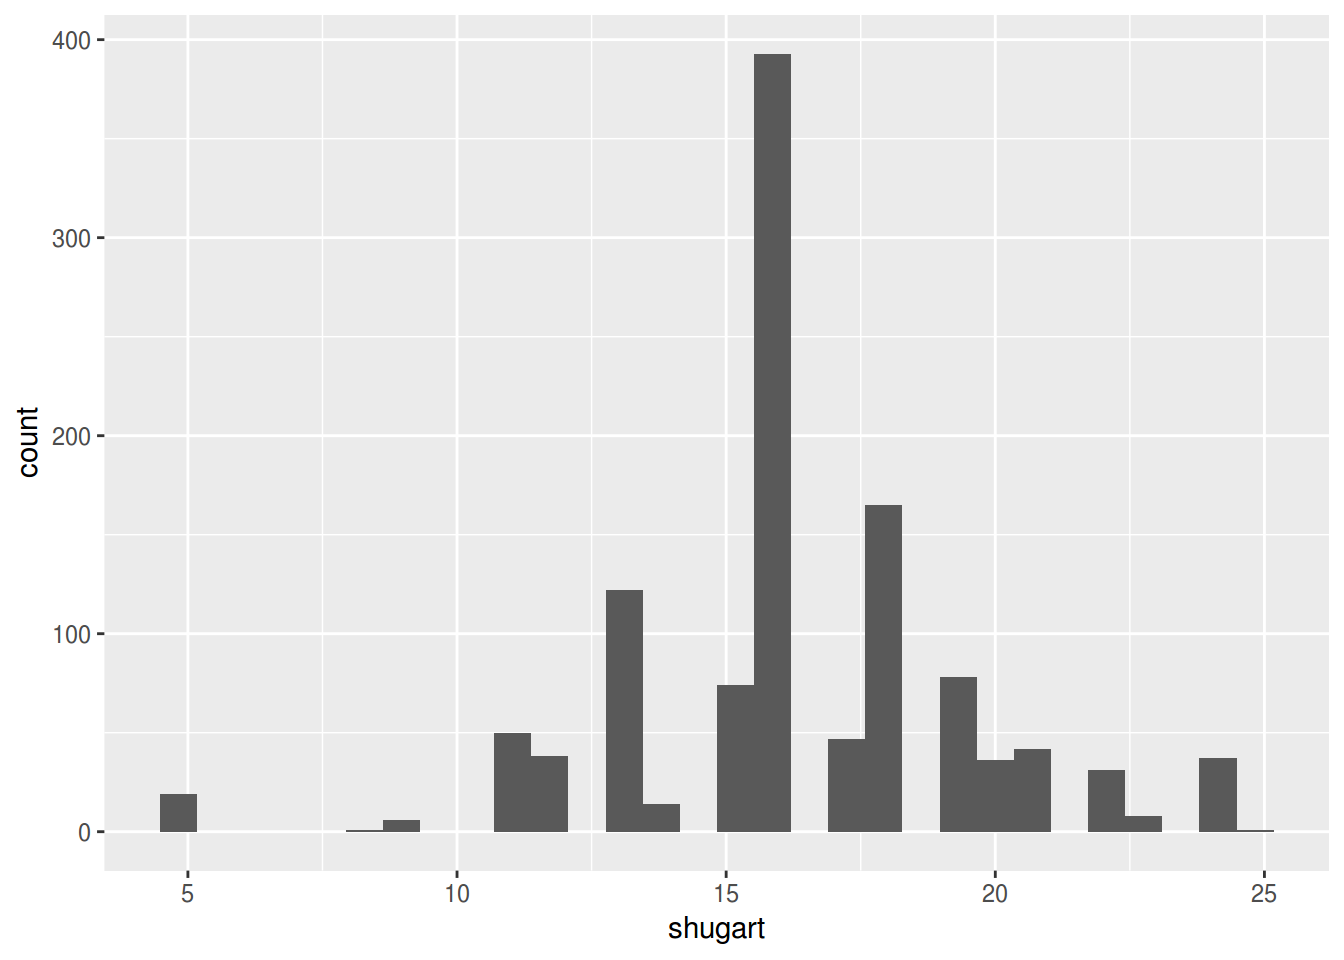
\includegraphics{adp-bookdown_files/figure-latex/unnamed-chunk-56-1} \end{center}

Tanto con \texttt{facet\_wrap} como con \texttt{facet\_grid} podemos
usar más de un argumento, pero los resultados son distintos.
\texttt{facet\_grid} no sólo ordena las geometrías, sino que es capaz de
cruzarlas creando gráficos con dos o más dimensiones utilizando
variables categóricas. Observen el siguiente ejemplo:

\texttt{facet\_wrap}

\begin{Shaded}
\begin{Highlighting}[]
\KeywordTok{ggplot}\NormalTok{(}\DataTypeTok{data    =}\NormalTok{ datos_municipales }\OperatorTok\StringTok{ }\KeywordTok{filter}\NormalTok{(year }\OperatorTok{==}\StringTok{ }\KeywordTok{c}\NormalTok{(}\DecValTok{2004}\NormalTok{, }\DecValTok{2008}\NormalTok{, }\DecValTok{2012}\NormalTok{)),}
       \DataTypeTok{mapping =} \KeywordTok{aes}\NormalTok{(}\DataTypeTok{x =}\NormalTok{ year, }\DataTypeTok{y =}\NormalTok{ casen)) }\OperatorTok{+}
\StringTok{  }\KeywordTok{geom_boxplot}\NormalTok{() }\OperatorTok{+}
\StringTok{  }\KeywordTok{facet_wrap}\NormalTok{(zona }\OperatorTok{~}\StringTok{ }\NormalTok{genero)}
\end{Highlighting}
\end{Shaded}

\begin{center}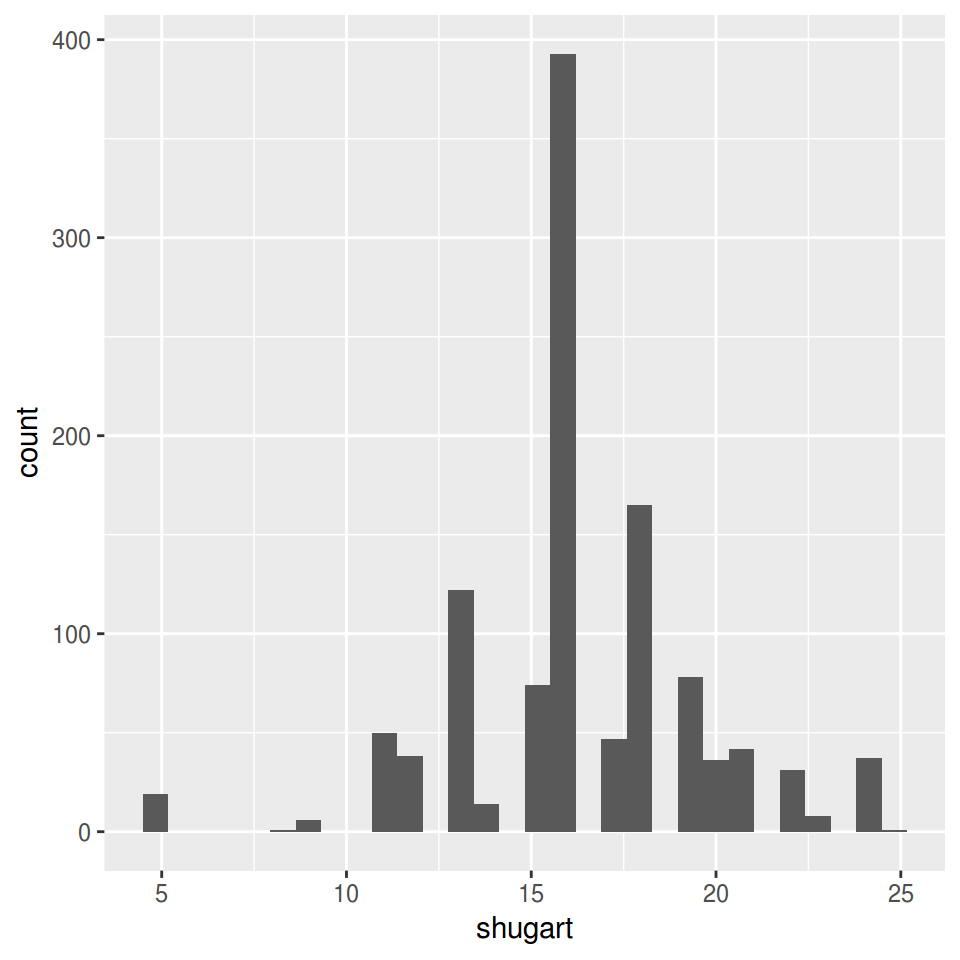
\includegraphics{adp-bookdown_files/figure-latex/unnamed-chunk-57-1} \end{center}

\texttt{facet\_grid}

\begin{Shaded}
\begin{Highlighting}[]
\KeywordTok{ggplot}\NormalTok{(}\DataTypeTok{data    =}\NormalTok{ datos_municipales }\OperatorTok\StringTok{ }\KeywordTok{filter}\NormalTok{(year }\OperatorTok{==}\StringTok{ }\KeywordTok{c}\NormalTok{(}\DecValTok{2004}\NormalTok{, }\DecValTok{2008}\NormalTok{, }\DecValTok{2012}\NormalTok{)),}
       \DataTypeTok{mapping =} \KeywordTok{aes}\NormalTok{(}\DataTypeTok{x =}\NormalTok{ year, }\DataTypeTok{y =}\NormalTok{ casen)) }\OperatorTok{+}
\StringTok{  }\KeywordTok{geom_boxplot}\NormalTok{() }\OperatorTok{+}
\StringTok{  }\KeywordTok{facet_grid}\NormalTok{(zona }\OperatorTok{~}\StringTok{ }\NormalTok{genero)}
\end{Highlighting}
\end{Shaded}

\begin{center}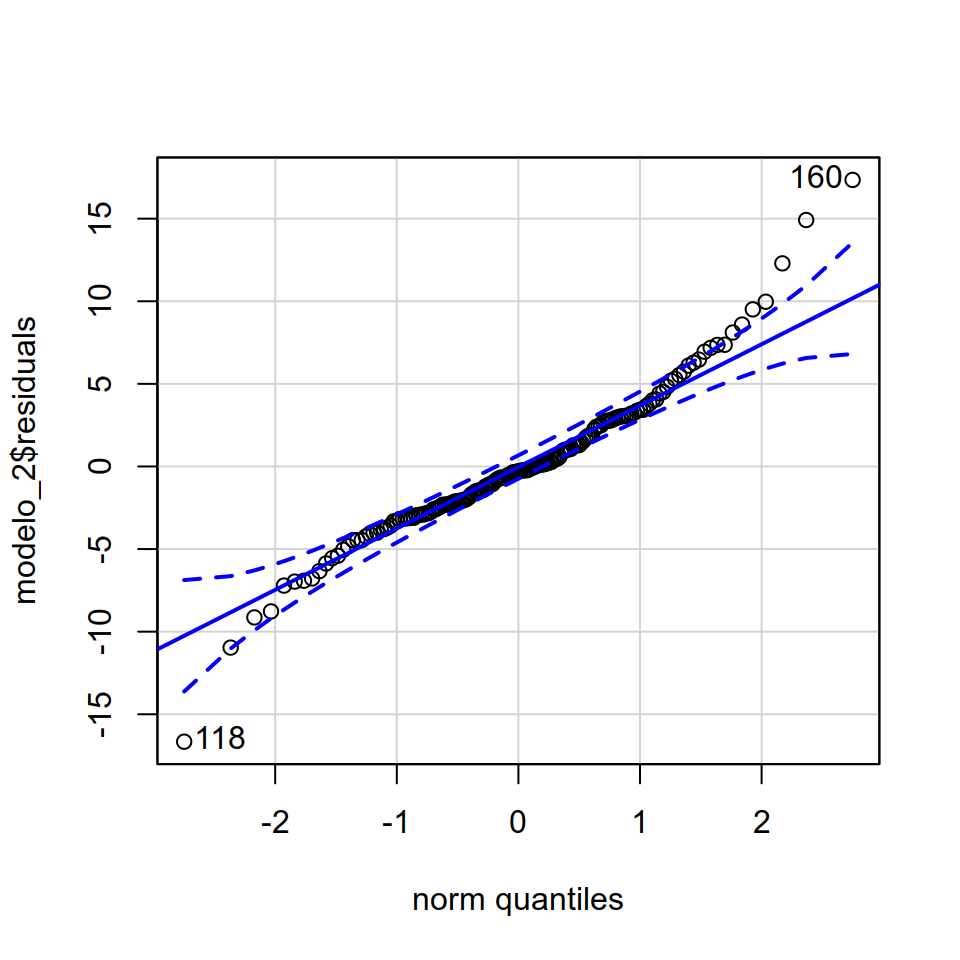
\includegraphics{adp-bookdown_files/figure-latex/unnamed-chunk-58-1} \end{center}

Este gráfico nos muestra que, por zona, el porcentaje de pobreza ha
variado considerablemente desde el 2004 al 2012 y que, hay una alta
variabilidad intraregional. Además, nos muestra cómo \texttt{ggplot}
entrega resultados de calidad sin mayores complejidades. La función
\texttt{facet\_wrap} es una capa opcional dentro de las múltiples capas
de ``A Layered Grammar of Graphics'', pero las otras tres deben estar
presentes para cualquier tipo de resultado.

\hypertarget{transformaciones}{%
\subsubsection{Transformaciones}\label{transformaciones}}

Otra capa que puedes utilizar es una capa que te permitirá hacer
transformaciones de escala en tus variables. Normalmente aparecerá con
el nombre \texttt{scale\_x\_discrete}, la cual va variando dependiendo
de la estética que estemos utilizando dentro de nuestro mapeo. Así,
podremos encontrarnos con \texttt{scale\_fill\_continuos} o
\texttt{scale\_y\_log10}. Por ejemplo, podemos ver cómo se distribuye el
ingreso de las municipalidades según el porcentaje de pobreza de nuestra
muestra. Normalmente esto lo haríamos de la siguiente manera:

\begin{Shaded}
\begin{Highlighting}[]
\KeywordTok{ggplot}\NormalTok{(}\DataTypeTok{data    =}\NormalTok{ datos_municipales }\OperatorTok\StringTok{ }\KeywordTok{filter}\NormalTok{(year }\OperatorTok{==}\StringTok{ }\KeywordTok{c}\NormalTok{(}\DecValTok{2004}\NormalTok{, }\DecValTok{2008}\NormalTok{, }\DecValTok{2012}\NormalTok{)),}
       \DataTypeTok{mapping =} \KeywordTok{aes}\NormalTok{(}\DataTypeTok{x =}\NormalTok{ casen, }\DataTypeTok{y =}\NormalTok{ ingresos)) }\OperatorTok{+}
\StringTok{  }\KeywordTok{geom_point}\NormalTok{() }
\end{Highlighting}
\end{Shaded}

\begin{center}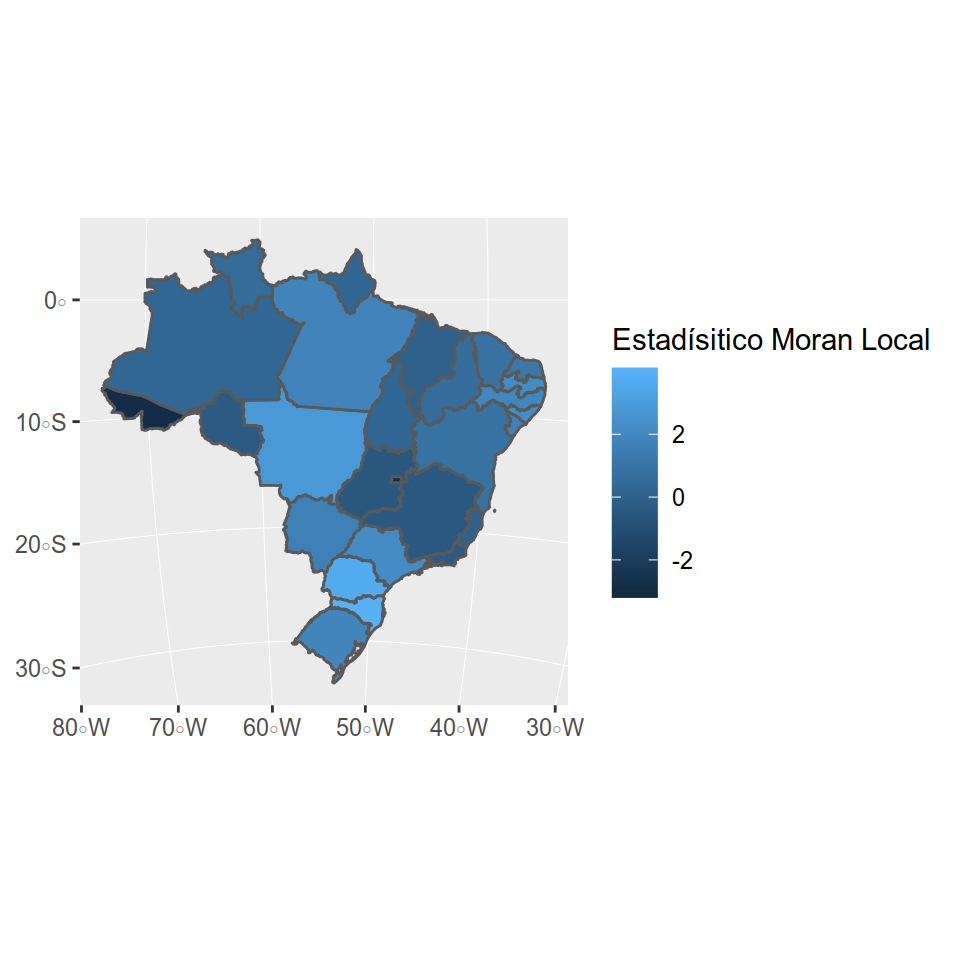
\includegraphics{adp-bookdown_files/figure-latex/unnamed-chunk-59-1} \end{center}

Teóricamente, cuando ocupamos una variable que tiene relación con
dinero, le aplicamos una transformación logarítmica. Pero ¿cómo se
traduce eso en nuestra imagen?

\begin{Shaded}
\begin{Highlighting}[]
\KeywordTok{ggplot}\NormalTok{(}\DataTypeTok{data    =}\NormalTok{ datos_municipales }\OperatorTok\StringTok{ }\KeywordTok{filter}\NormalTok{(year }\OperatorTok{==}\StringTok{ }\KeywordTok{c}\NormalTok{(}\DecValTok{2004}\NormalTok{, }\DecValTok{2008}\NormalTok{, }\DecValTok{2012}\NormalTok{)),}
       \DataTypeTok{mapping =} \KeywordTok{aes}\NormalTok{(}\DataTypeTok{x =}\NormalTok{ casen, }\DataTypeTok{y =}\NormalTok{ ingresos)) }\OperatorTok{+}
\StringTok{  }\KeywordTok{geom_point}\NormalTok{() }\OperatorTok{+}
\StringTok{  }\KeywordTok{scale_y_log10}\NormalTok{()}
\end{Highlighting}
\end{Shaded}

\begin{center}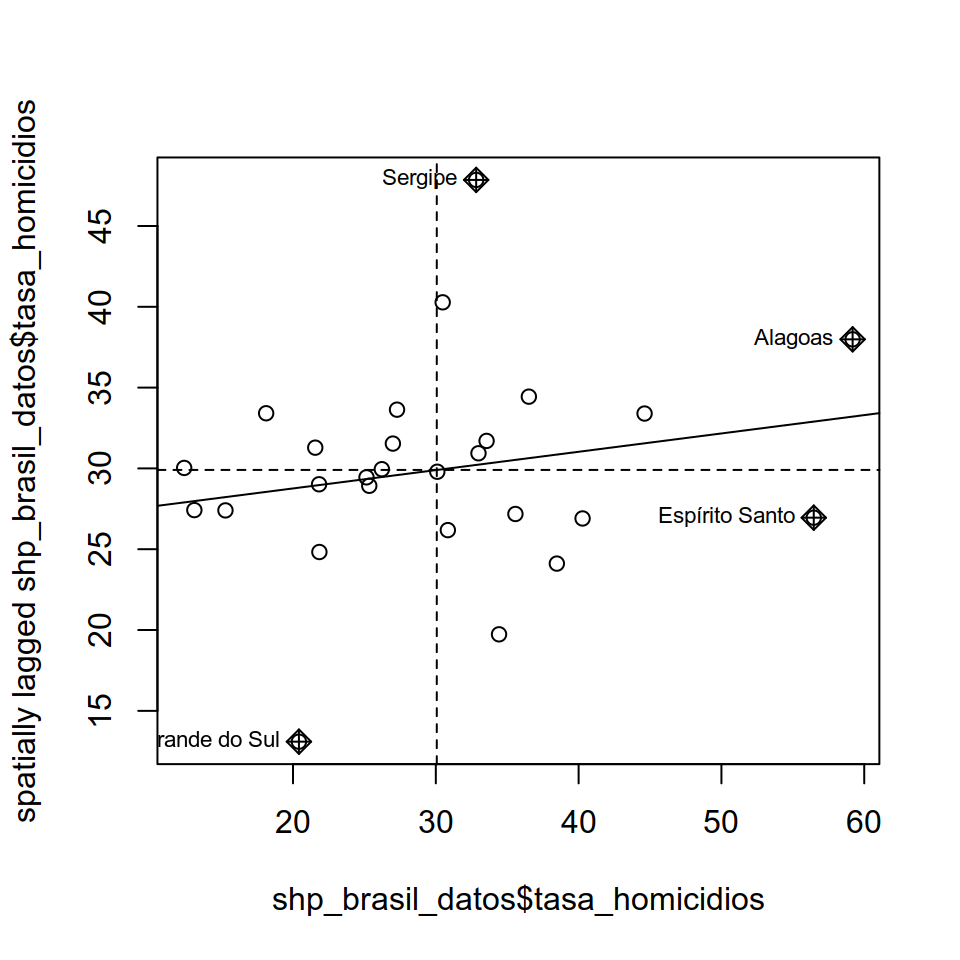
\includegraphics{adp-bookdown_files/figure-latex/unnamed-chunk-60-1} \end{center}

Esto es de lo que hablamos cuando hablamos de escalas.

\hypertarget{sistema-de-coordenadas}{%
\subsubsection{Sistema de coordenadas}\label{sistema-de-coordenadas}}

Normalmente, trabajaremos con un eje x y un eje y. Existen funciones en
\texttt{ggplot2} como \texttt{coord\_flip} que nos permitirá cambiar el
sentido de nuestro gráfico. Pero también usamos este tipo de capa cuando
trabajamos con datos geográficos o cuando, por ejemplo, queremos hacer
un gráfico de torta. Aunque, normalmente,
\href{https://www.datapine.com/blog/common-data-visualization-mistakes/}{no
queremos hacer gráficos de torta}. Entre más utilices \texttt{ggplot2},
más aprenderás de cada una de las opciones.

\hypertarget{temas}{%
\subsubsection{Temas}\label{temas}}

Cuando mapeamos los datos, usamos opciones estéticas. Cuando queremos
cambiar cómo luce el gráfico, cambiamos el tema. Esto se puede hacer a
través de \texttt{theme}, el cual te permite modificar cuestiones que no
se relacionan con el contenido del grafico. Por ejemplo, los colores del
fondo o el tipo de letras de los ejes. También puedes cambiar dónde se
ubicará la leyenda o la ubicación del título. También, puedes cambiar el
título, el nombre de los ejes, agregar anotaciones, etc. Solo necesitas
conocer \texttt{labs}, \texttt{annotate} y \texttt{ggtitle}.

Ahora, a aplicar todo lo que \emph{al parecer} entendemos.

\#\#3. Elecciones locales y visualización de datos

Como habíamos mencionado, lo principal es entender que la visualización
nos sirve para explorar nuestros datos y contestar preguntas sustantivas
de nuestra investigación. Muchas veces las medias, desviaciones estándar
u otro tipo de parámetro no nos dice mucho. Esos mismos datos podemos
expresarlos a través de la visualización. Por ejemplo, un boxplot puede
ser útil para representar la distribución de los datos que tenemos y ver
sus posibles outliers, mientras que un gráfico de barras nos ayudará a
ver la frecuencia de nuestros datos categóricos, y un gráfico de línea
nos sirve para entender cambios en el tiempo. Y esos son sólo algunos
ejemplos dentro de una variada gama de posibilidades.

En esta tercera parte, aprenderemos a visualizar diferentes tipos de
gráficos con los datos de reelección municipal en Chile. En resumen, en
Chile la divisón político-administrativa más pequeña es la comuna o
municipio que cada cuatro años escoge a sus autoridades locales: un
alcalde y un concejo municipal. Desde 1992 al 2000, los alcaldes fueron
electos de forma indirecta, y desde el 2004 en adelante empiezan a ser
electos directamente por la ciudadanía. Ya que conocemos nuestros datos,
podemos empezar por lo más simple. Una buena idea, por ejemplo, es ver
la cantidad de mujeres electas como alcaldesas versus el número de
hombres electos. Para eso, podemos usar un gráfico de barras. Como bien
vimos en el ítem anterior, para armar cualquier tipo de gráfico
necesitamos conocer la o las variables que queremos usar y cuál
geometría o \texttt{geom} nos permite representar lo que queremos
conocer. En este caso, usaremos \texttt{geom\_bar} para ver cuántos
hombres y cuántas mujeres han sido electos desde 1992.

\hypertarget{grafico-de-barras}{%
\subsection{Gráfico de barras}\label{grafico-de-barras}}

\begin{Shaded}
\begin{Highlighting}[]
\NormalTok{plot_a <-}\StringTok{ }\KeywordTok{ggplot}\NormalTok{(datos_municipales, }\DataTypeTok{mapping =} \KeywordTok{aes}\NormalTok{(}\DataTypeTok{x =}\NormalTok{ genero))}

\NormalTok{plot_a }\OperatorTok{+}\StringTok{ }\KeywordTok{geom_bar}\NormalTok{()}
\end{Highlighting}
\end{Shaded}

\begin{center}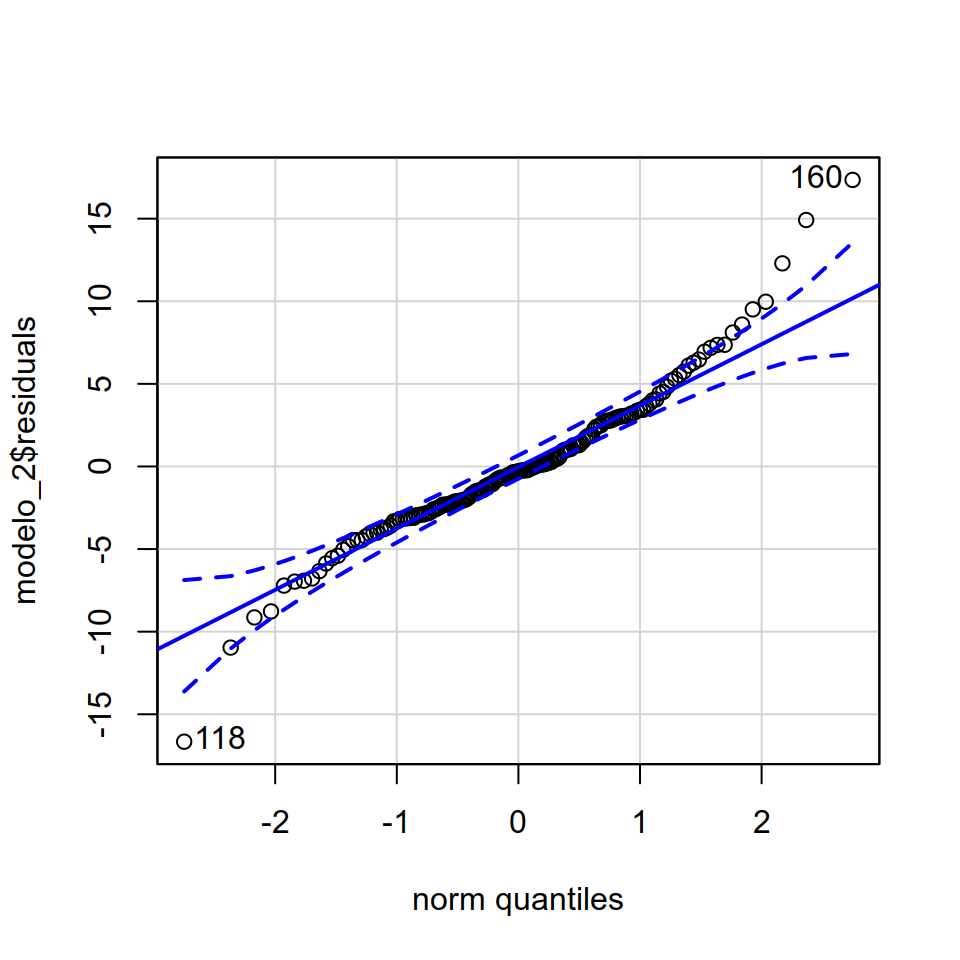
\includegraphics{adp-bookdown_files/figure-latex/unnamed-chunk-61-1} \end{center}

Como vemos, armar un gráfico de barras es muy simple. Podemos ver que,
desde 1992, han sido electos más de 1500 hombres como alcaldes, una
cifra que supera largamente a las menos 250 mujeres que han sido electas
para el mismo cargo en la misma cantidad de tiempo.

Pero, quizás, esto no se mantiene por zona: ¿Qué pasa cuando
subdividimos el gráfico para ver qué pasa por zona geográfica?

\begin{Shaded}
\begin{Highlighting}[]
\NormalTok{plot_a }\OperatorTok{+}\StringTok{ }
\StringTok{  }\KeywordTok{geom_bar}\NormalTok{() }\OperatorTok{+}\StringTok{ }
\StringTok{  }\KeywordTok{facet_wrap}\NormalTok{(}\OperatorTok{~}\NormalTok{zona, }\DataTypeTok{nrow =} \DecValTok{1}\NormalTok{)}
\end{Highlighting}
\end{Shaded}

\begin{center}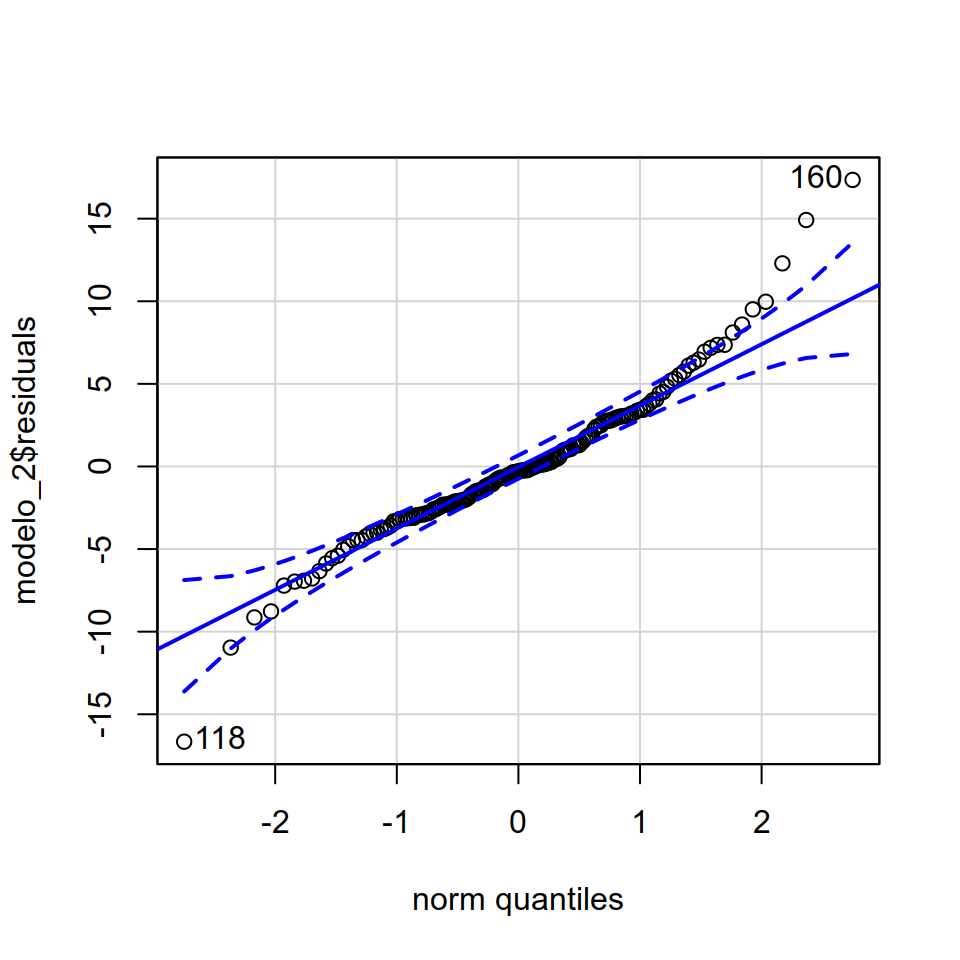
\includegraphics{adp-bookdown_files/figure-latex/unnamed-chunk-62-1} \end{center}

Uno de los problemas con este gráfico, es que no tiene en consideración
el número de comunas por cada zona. Mientras que en el norte de Chile
hay, en general, pocas comunas, en la zona central podemos encontrar que
sólo la Región Metropolitana cuenta con más de 52. Sin considerar las
otras cinco regiones que componen la zona. Quizás, sería más prudente si
vemos la proporción de mujeres y hombres electos por zona.

\begin{Shaded}
\begin{Highlighting}[]
\NormalTok{plot_a }\OperatorTok{+}\StringTok{ }
\StringTok{  }\KeywordTok{geom_bar}\NormalTok{(}\DataTypeTok{mapping =} \KeywordTok{aes}\NormalTok{(}\DataTypeTok{y =}\NormalTok{ ..prop..)) }\OperatorTok{+}
\StringTok{  }\KeywordTok{facet_wrap}\NormalTok{(}\OperatorTok{~}\NormalTok{zona, }\DataTypeTok{nrow =} \DecValTok{1}\NormalTok{)}
\end{Highlighting}
\end{Shaded}

\begin{center}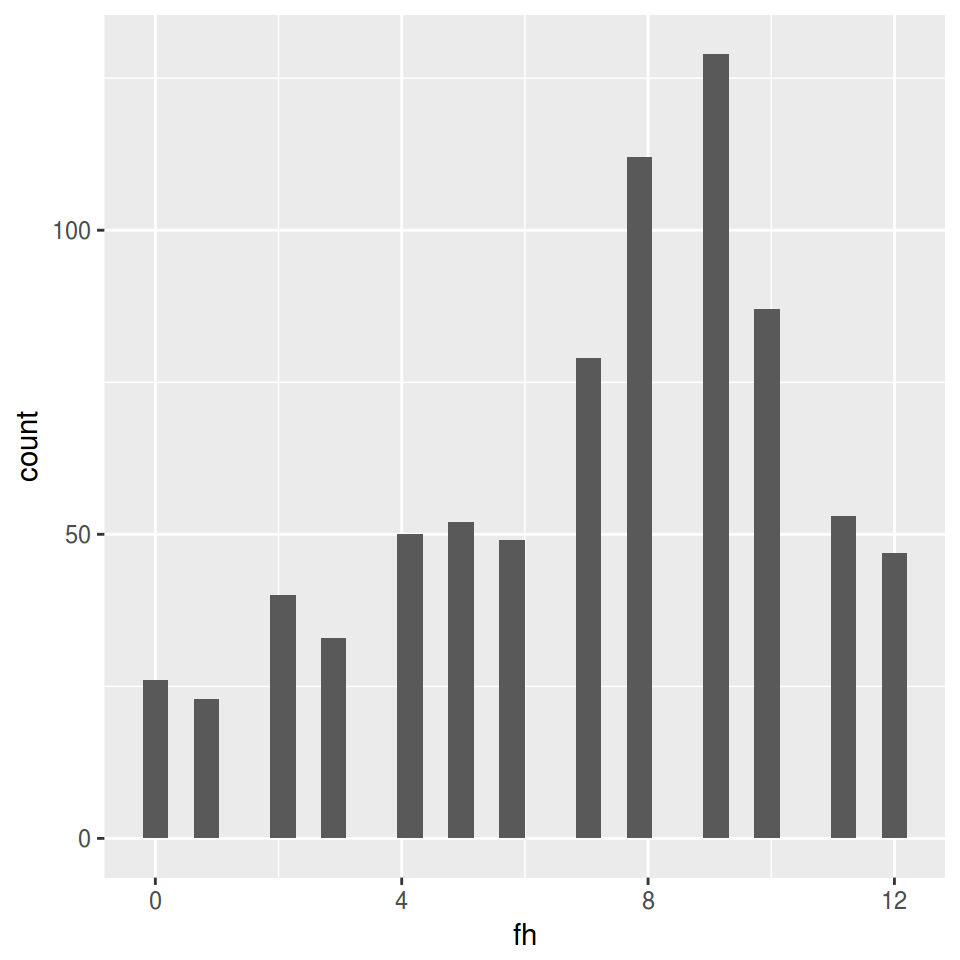
\includegraphics{adp-bookdown_files/figure-latex/unnamed-chunk-63-1} \end{center}

Las geometrías \texttt{geom\_bar} o \texttt{geom\_col},
\texttt{geom\_density} y \texttt{geom\_histogram} no suelen llevar el
eje y explicitado en las estéticas, ya que son un conteo sobre el eje x.
Al especificar \texttt{y\ =\ ..prop..} como estética dentro del objeto
geométrico, estamos ordenando el cálculo de la proporción, no la cuenta.
Normalmente, usaremos \texttt{aes()} en conjunto con los datos en
\texttt{ggplot()}, pero dependiendo de la preferencia que tengas, es
posible usarlo también con los \texttt{geom}. Esto último es más común
cuando ocupamos más de una base de datos o cuando queremos hacer algún
tipo de transformación.

A pesar de lograr la transformación, como apreciamos en las etiquetas
del eje y, no conseguimos lo que queríamos. No es un error de nosotros,
sino que es una característica de la función \texttt{geom\_bar}. Cuando
hacemos un gráfico de barras, la función cuenta la frecuencia de cada
característica en la base de datos. Así, por ejemplo, en el Norte Chico
han sido electos 101 hombres desde 1992 versus 20 mujeres. En el Norte
Grande, han sido electos 89 hombres versus 13 mujeres, y así. Pero
cuando calculamos la proporción, la función no la calcula en base a la
suma de ambos por zona, sino en base a sí misma. Suena complejo, pero no
lo es. En este caso, ve que hay 89 hombres electos en el Norte Grande y
la función dice ``en el Norte Grande los 89 hombres corresponden al
100\% de hombres, y las 13 mujeres corresponden al 100\% de mujeres'',
cuando lo que queremos saber qué porcentaje del total de alcaldes son
hombres y qué porcentaje son mujeres.

Para eso utilizamos \texttt{group\ =\ 1}.

\begin{Shaded}
\begin{Highlighting}[]
\NormalTok{plot_a }\OperatorTok{+}\StringTok{ }
\StringTok{  }\KeywordTok{geom_bar}\NormalTok{(}\DataTypeTok{mapping =} \KeywordTok{aes}\NormalTok{(}\DataTypeTok{y =}\NormalTok{ ..prop.., }\DataTypeTok{group =} \DecValTok{1}\NormalTok{)) }\OperatorTok{+}
\StringTok{  }\KeywordTok{facet_wrap}\NormalTok{(}\OperatorTok{~}\NormalTok{zona, }\DataTypeTok{nrow =} \DecValTok{1}\NormalTok{)}
\end{Highlighting}
\end{Shaded}

\begin{center}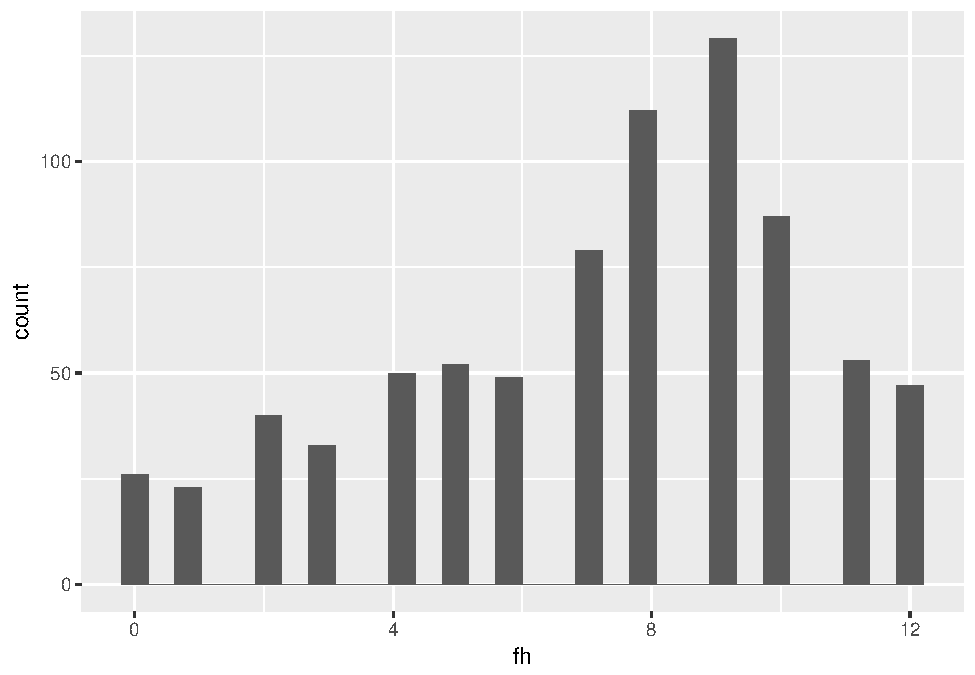
\includegraphics{adp-bookdown_files/figure-latex/unnamed-chunk-64-1} \end{center}

¡Ahora sí lo logramos! Vemos que no hay grandes diferencias, siendo el
``Norte Chico'' el que cuenta con más mujeres en la alcaldía en relación
a los hombres. A pesar de esto, no hay grandes diferencias de zona a
zona y parece que se replicaran los resultados que vimos en nuestro
primer gráfico de barras. Ahora, podríamos arreglar temas estéticos del
gráfico. Por ejemplo, ponerle título, la fuente de los datos y
especificar qué es 0 y qué es 1.

\begin{Shaded}
\begin{Highlighting}[]
\NormalTok{plot_a }\OperatorTok{+}\StringTok{ }
\StringTok{  }\KeywordTok{geom_bar}\NormalTok{(}\DataTypeTok{mapping =} \KeywordTok{aes}\NormalTok{(}\DataTypeTok{y =}\NormalTok{ ..prop.., }\DataTypeTok{group =} \DecValTok{1}\NormalTok{)) }\OperatorTok{+}
\StringTok{  }\KeywordTok{facet_wrap}\NormalTok{(}\OperatorTok{~}\NormalTok{zona, }\DataTypeTok{nrow =} \DecValTok{1}\NormalTok{) }\OperatorTok{+}
\StringTok{  }\KeywordTok{labs}\NormalTok{(}\DataTypeTok{title =} \StringTok{"Proporción de mujeres y hombres electos alcaldes (1992-2012)}\CharTok{\textbackslash{}n}\StringTok{Por zonas económicas de Chile"}\NormalTok{, }
       \DataTypeTok{x =} \StringTok{"Género"}\NormalTok{, }\DataTypeTok{y =} \StringTok{"Proporción", }
\StringTok{       caption = "}\NormalTok{Fuente}\OperatorTok{:}\StringTok{ }\NormalTok{base de elaboración propia con datos del SERVEL y }\KeywordTok{SINIM}\NormalTok{ (}\DecValTok{2018}\NormalTok{)}\StringTok{") }
\end{Highlighting}
\end{Shaded}

\begin{center}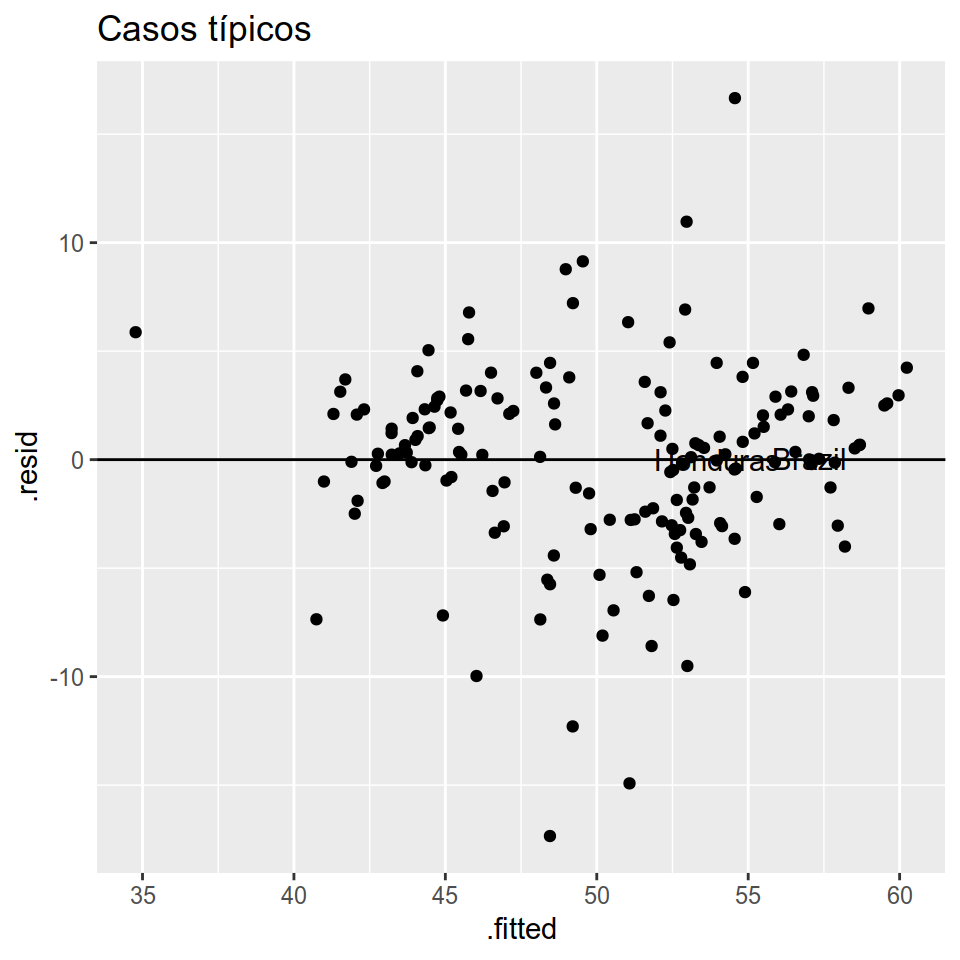
\includegraphics{adp-bookdown_files/figure-latex/unnamed-chunk-65-1} \end{center}

Ahora, sólo nos falta agregar las etiquetas del eje x. Eso lo podemos
hacer fácilemente con \texttt{scale\_x\_discrete}. Tienes que tener en
consideración qué estética de \texttt{aes()} modificarás, ya que eso
cambiará el \texttt{scale} que necesites. Si estuviéramos viendo las
etiquetas de \texttt{fill}, tendríamos que usar
\texttt{scale\_fill\_discrete}, por ejemplo. También tienes que tener en
consideración qué tipo de variable estás usando. Que
\texttt{scale\_x\_dicrete} tenga ``discrete'' al final no es una
decisión aleatoria. Como comprenderás, depende totalmente del tipo de
variable que estemos manejando.

\begin{Shaded}
\begin{Highlighting}[]
\NormalTok{plot_a }\OperatorTok{+}\StringTok{ }
\StringTok{  }\KeywordTok{geom_bar}\NormalTok{(}\DataTypeTok{mapping =} \KeywordTok{aes}\NormalTok{(}\DataTypeTok{y =}\NormalTok{ ..prop.., }\DataTypeTok{group =} \DecValTok{1}\NormalTok{)) }\OperatorTok{+}
\StringTok{  }\KeywordTok{facet_wrap}\NormalTok{(}\OperatorTok{~}\NormalTok{zona, }\DataTypeTok{nrow =} \DecValTok{1}\NormalTok{) }\OperatorTok{+}
\StringTok{  }\KeywordTok{scale_x_discrete}\NormalTok{(}\DataTypeTok{labels =} \KeywordTok{c}\NormalTok{(}\StringTok{"Hombres"}\NormalTok{, }\StringTok{"Mujeres"}\NormalTok{)) }\OperatorTok{+}
\StringTok{  }\KeywordTok{labs}\NormalTok{(}\DataTypeTok{title =} \StringTok{"Proporción de mujeres y hombres electos alcaldes (1992-2012)}\CharTok{\textbackslash{}n}\StringTok{Por zonas económicas de Chile"}\NormalTok{, }
       \DataTypeTok{x =} \StringTok{"Género"}\NormalTok{, }\DataTypeTok{y =} \StringTok{"Proporción", }
\StringTok{       caption = "}\NormalTok{Fuente}\OperatorTok{:}\StringTok{ }\NormalTok{base de elaboración propia con datos del SERVEL y }\KeywordTok{SINIM}\NormalTok{ (}\DecValTok{2018}\NormalTok{)}\StringTok{") }
\end{Highlighting}
\end{Shaded}

\begin{center}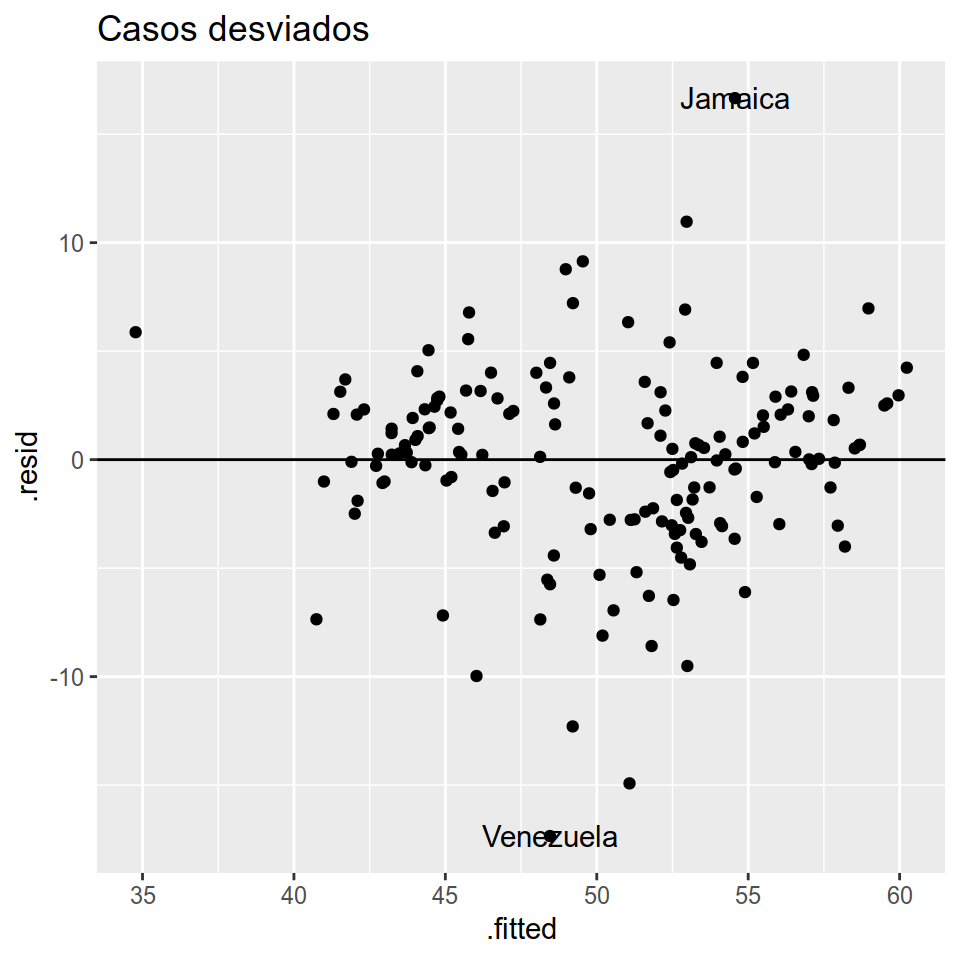
\includegraphics{adp-bookdown_files/figure-latex/unnamed-chunk-66-1} \end{center}

Con \texttt{labels} podemos cambiar las etiquetas. Ten en consideración
el número de \texttt{breaks} de tu variable categórica para que calcen a
la perfección y no te sobre (o te falte) alguna categoría.

Ejercicio:

\begin{itemize}
\tightlist
\item
  \texttt{geom\_bar} suele ser un poco inflexible. Puedes obtener los
  mismos resultados y con mayor plasticidad utilizando
  \texttt{geom\_col}.
\item
  Sería interesante cambiar el color de las barras para que éstas
  expresen la categoría género. Una opción es hacerlo a través de la
  estética \texttt{fill} al mapear los datos en \texttt{aes()}.
\item
  Para ver los cambios anuales de estas cifras, cambia ``zona'' por
  ``year'' \texttt{facet\_wrap} ¿qué tendencia ves?
\end{itemize}

\begin{Shaded}
\begin{Highlighting}[]
\NormalTok{plot_a }\OperatorTok{+}\StringTok{ }
\StringTok{  }\KeywordTok{geom_bar}\NormalTok{(}\DataTypeTok{mapping =} \KeywordTok{aes}\NormalTok{(}\DataTypeTok{y =}\NormalTok{ ..prop.., }\DataTypeTok{group =} \DecValTok{1}\NormalTok{)) }\OperatorTok{+}
\StringTok{  }\KeywordTok{facet_wrap}\NormalTok{(}\OperatorTok{~}\NormalTok{year, }\DataTypeTok{nrow =} \DecValTok{1}\NormalTok{) }\OperatorTok{+}
\StringTok{  }\KeywordTok{scale_x_discrete}\NormalTok{(}\DataTypeTok{labels =} \KeywordTok{c}\NormalTok{(}\StringTok{"Hombres"}\NormalTok{, }\StringTok{"Mujeres"}\NormalTok{)) }\OperatorTok{+}
\StringTok{  }\KeywordTok{labs}\NormalTok{(}\DataTypeTok{title =} \StringTok{"Proporción de mujeres y hombres electos alcaldes (1992-2012)}\CharTok{\textbackslash{}n}\StringTok{Por zonas económicas de Chile"}\NormalTok{, }
       \DataTypeTok{x =} \StringTok{"Género"}\NormalTok{, }\DataTypeTok{y =} \StringTok{"Proporción", }
\StringTok{       caption = "}\NormalTok{Fuente}\OperatorTok{:}\StringTok{ }\NormalTok{base de elaboración propia con datos del SERVEL y }\KeywordTok{SINIM}\NormalTok{ (}\DecValTok{2018}\NormalTok{)}\StringTok{")}
\end{Highlighting}
\end{Shaded}

\begin{center}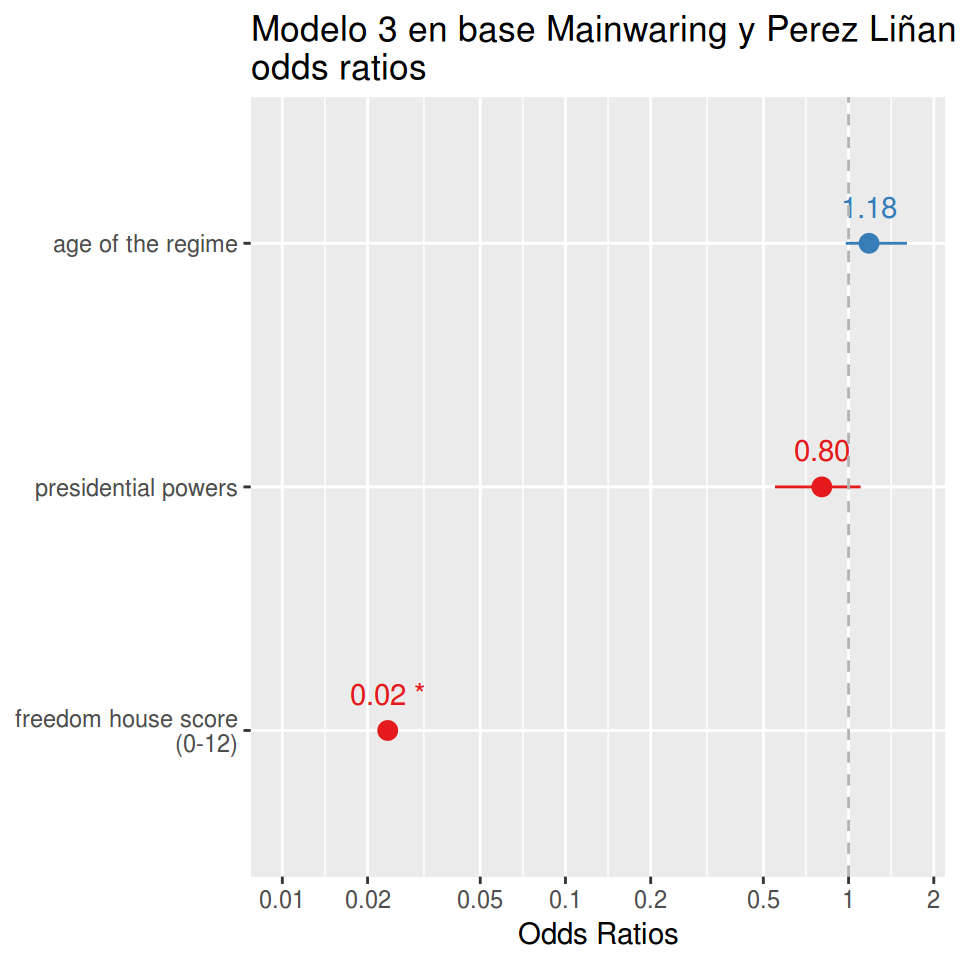
\includegraphics{adp-bookdown_files/figure-latex/unnamed-chunk-67-1} \end{center}

\#\#\#Gráfico de Línea

En el gráfico final de la sección anterior, vimos que si bien la
elección de mujeres alcaldesas en Chile ha aumentado, este no parece ser
significativo: en el 2012, sólo un 13\% de los alcaldes electos eran
mujeres. Quizás esto puede deberse a que los cambios socioeconómicos no
han repercutido en la percepción sobre los roles de género en la
sociedad. Tal vez, mirar los datos económicos de ingresos municipales o
de porcentaje de pobreza según la CASEN nos ayuden a entender por qué no
ha aumentado sustantivamente la elección de mujeres en las elecciones
municipales. Para esto podemos usar \texttt{geom\_line}, el objeto
geométrico que nos permitirá ver la evolución en el tiempo de nuestro
objeto de estudio. La intuición sería hacer la figura de esta manera:

\begin{Shaded}
\begin{Highlighting}[]
\NormalTok{plot_b <-}\StringTok{ }\KeywordTok{ggplot}\NormalTok{(}\DataTypeTok{data    =}\NormalTok{ datos_municipales, }
                 \DataTypeTok{mapping =} \KeywordTok{aes}\NormalTok{(}\DataTypeTok{x =}\NormalTok{ year, }\DataTypeTok{y =}\NormalTok{ ingresos)) }

\NormalTok{plot_b }\OperatorTok{+}\StringTok{ }
\StringTok{  }\KeywordTok{geom_line}\NormalTok{()}
\end{Highlighting}
\end{Shaded}

\begin{center}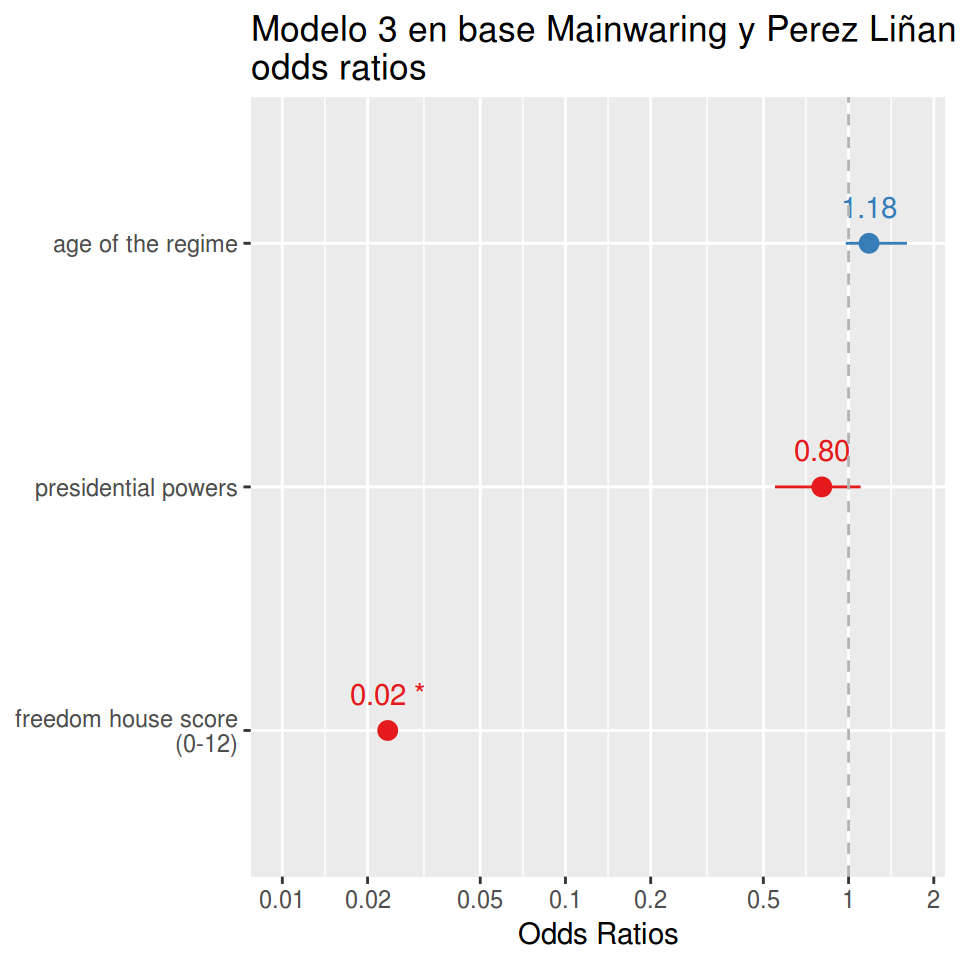
\includegraphics{adp-bookdown_files/figure-latex/unnamed-chunk-68-1} \end{center}

El problema es que no nos entrega el resultado esperado. La intuición es
correcta, pero nosotros tenemos que ayudar a \texttt{geom\_line} con
ciertas especificaciones. \texttt{geom\_line} agrupa las observaciones
para crear el gráfico de línea. En este caso, las agrupa por lo que cree
tiene más sentido: el año. Por esta razón, tenemos que especificar cuál
es la variable que agrupa toda la información y como sabemos, la
información que tenemos está agrupada por municipio. Cuando agregamos
esta información como \texttt{geom\_lines(aes(group\ =\ comuna))}, el
resultado cambia y se asemeja a lo que buscábamos:

\begin{Shaded}
\begin{Highlighting}[]
\NormalTok{plot_b }\OperatorTok{+}\StringTok{ }
\StringTok{  }\KeywordTok{geom_line}\NormalTok{(}\DataTypeTok{mapping =} \KeywordTok{aes}\NormalTok{(}\DataTypeTok{group =}\NormalTok{ comuna))}
\end{Highlighting}
\end{Shaded}

\begin{center}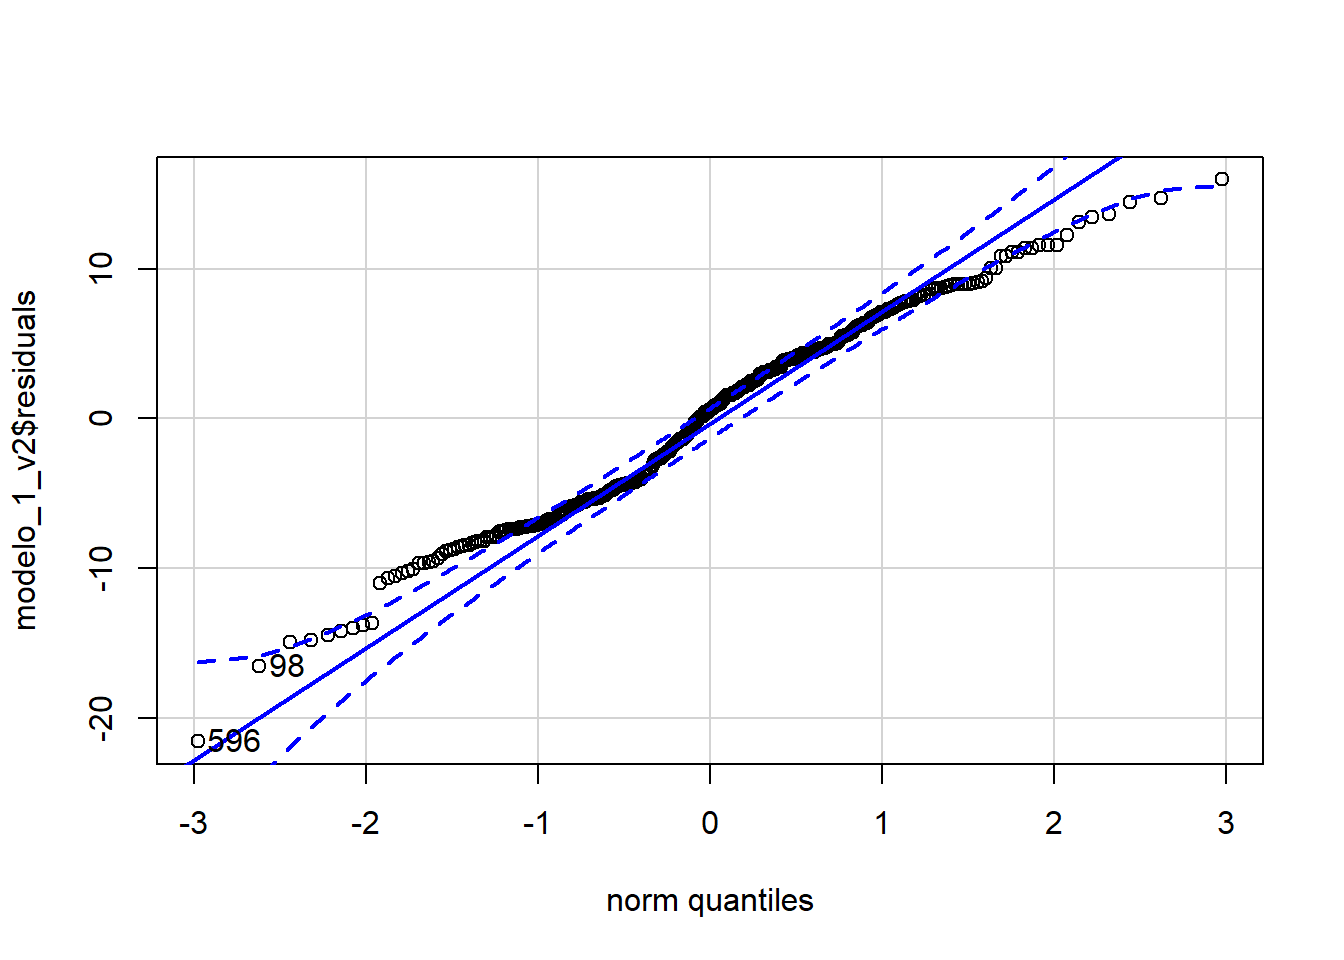
\includegraphics{adp-bookdown_files/figure-latex/unnamed-chunk-69-1} \end{center}

Dos problemas que surgen a simple vista:

\begin{enumerate}
\def\labelenumi{\arabic{enumi}.}
\tightlist
\item
  No tenemos datos anteriores al 2004.
\item
  Considerando que son 345 comunas, parece imposible tenerlas todas en
  un solo gráfico.
\end{enumerate}

Estos dos problemas se pueden solucionar fácilmente. Primero, queremos
eliminar los periodos anteriores al 2004. Para hacer esto, tenemos dos
posible soluciones:

La primera solución es simplemente hacer un subset de la variable con
\texttt{filter}, combinando las herramientas del \texttt{tidyverse} y
las de \texttt{ggplot}. En este caso, seleccionamos solo los años que
utilizaremos para la construcción del gráfico, dejando afuera 1992, 1996
y 2000. Para seleccionar más de un nivel en una variable, utilizamos
\texttt{\%in\%}. Finalmente, tenemos el resultado deseado:

\begin{Shaded}
\begin{Highlighting}[]
\KeywordTok{ggplot}\NormalTok{(}\DataTypeTok{data    =}\NormalTok{ datos_municipales }\OperatorTok\StringTok{ }\KeywordTok{filter}\NormalTok{(year }\OperatorTok\StringTok{ }\KeywordTok{c}\NormalTok{(}\DecValTok{2004}\NormalTok{, }\DecValTok{2008}\NormalTok{, }\DecValTok{2012}\NormalTok{)),}
       \DataTypeTok{mapping =} \KeywordTok{aes}\NormalTok{(}\DataTypeTok{x =}\NormalTok{ year, }\DataTypeTok{y =}\NormalTok{ ingresos)) }\OperatorTok{+}
\StringTok{  }\KeywordTok{geom_line}\NormalTok{(}\KeywordTok{aes}\NormalTok{(}\DataTypeTok{group =}\NormalTok{ comuna))}
\end{Highlighting}
\end{Shaded}

\begin{center}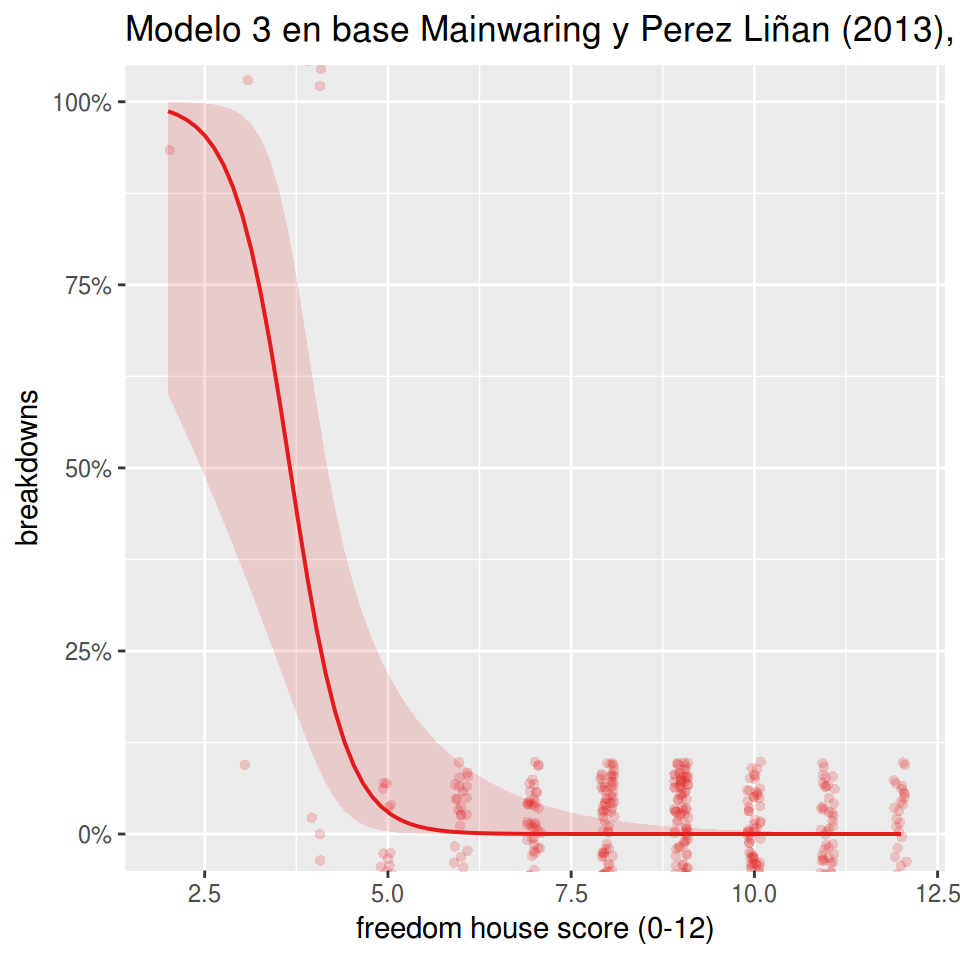
\includegraphics{adp-bookdown_files/figure-latex/unnamed-chunk-70-1} \end{center}

Ahora, podemos separar el gráfico como lo habíamos hecho anteriormente.
Se puede hacer por zona o por región, pensando en cuál resultado te
interesa más. Ya que hemos visto diferentes resultados por zonas, sería
interesante ver el ingreso de la misma manera.

\begin{Shaded}
\begin{Highlighting}[]
\NormalTok{plot_b }\OperatorTok{+}\StringTok{ }
\StringTok{  }\KeywordTok{geom_line}\NormalTok{(}\KeywordTok{aes}\NormalTok{(}\DataTypeTok{group =}\NormalTok{ comuna)) }\OperatorTok{+}
\StringTok{  }\KeywordTok{facet_wrap}\NormalTok{(}\OperatorTok{~}\NormalTok{zona, }\DataTypeTok{nrow =} \DecValTok{1}\NormalTok{)}
\end{Highlighting}
\end{Shaded}

\begin{center}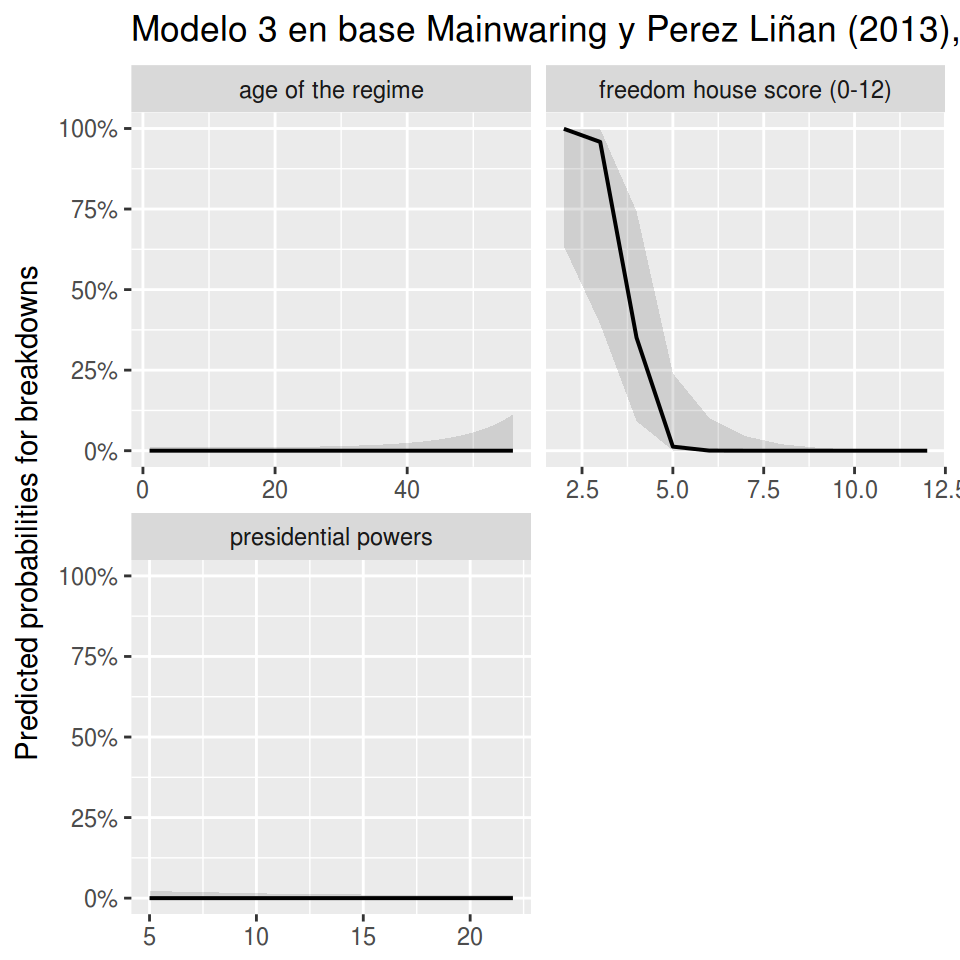
\includegraphics{adp-bookdown_files/figure-latex/unnamed-chunk-71-1} \end{center}

Como son pocos años, no podemos ver mucha variabilidad y a primera
vista, parece que los ingresos de todos los municipios han incrementado
considerablemente. Quizás, podemos seguir mejorando nuestro gráfico.
Probablemente, no estés muy familiarizado con la notación científica y
te sientes más cómodo leyendo números más grandes. Quizás sabes que es
mejor trabajar todo tipo de variable monetaria con su transformación
logarítmica, como nos han enseñado en diferentes cursos de métodologías.
Puede, también, que quieras agregar otro tipo de información a este
gráfico, como por ejemplo, las medias.

¿Qué te parece el siguiente gráfico?

\begin{Shaded}
\begin{Highlighting}[]
\NormalTok{medias <-}\StringTok{ }\NormalTok{datos_municipales }\OperatorTok\StringTok{ }
\StringTok{  }\KeywordTok{group_by}\NormalTok{(zona) }\OperatorTok\StringTok{ }
\StringTok{  }\KeywordTok{summarise}\NormalTok{(}\DataTypeTok{mean =} \KeywordTok{mean}\NormalTok{(ingresos, }\DataTypeTok{na.rm =}\NormalTok{ T))}

\NormalTok{plot_b }\OperatorTok{+}\StringTok{ }
\StringTok{  }\KeywordTok{geom_line}\NormalTok{(}\DataTypeTok{color =} \StringTok{"gray70"}\NormalTok{, }\KeywordTok{aes}\NormalTok{(}\DataTypeTok{group =}\NormalTok{ comuna)) }\OperatorTok{+}
\StringTok{  }\KeywordTok{geom_hline}\NormalTok{(}\KeywordTok{aes}\NormalTok{(}\DataTypeTok{yintercept =}\NormalTok{ mean), }\DataTypeTok{data =}\NormalTok{ medias, }\DataTypeTok{color =} \StringTok{"dodgerblue3"}\NormalTok{) }\OperatorTok{+}
\StringTok{  }\KeywordTok{scale_x_discrete}\NormalTok{(}\DataTypeTok{expand =} \KeywordTok{c}\NormalTok{(}\DecValTok{0}\NormalTok{,}\DecValTok{0}\NormalTok{)) }\OperatorTok{+}
\StringTok{  }\KeywordTok{scale_y_log10}\NormalTok{(}\DataTypeTok{labels =}\NormalTok{ scales}\OperatorTok{::}\NormalTok{dollar) }\OperatorTok{+}
\StringTok{  }\KeywordTok{facet_wrap}\NormalTok{(}\OperatorTok{~}\StringTok{ }\NormalTok{zona, }\DataTypeTok{nrow =} \DecValTok{1}\NormalTok{) }\OperatorTok{+}
\StringTok{  }\KeywordTok{labs}\NormalTok{(}\DataTypeTok{title =} \StringTok{"Ingresos municipales en años electorales (2004-2012)"}\NormalTok{,}
       \DataTypeTok{y =} \StringTok{"Ingresos"}\NormalTok{,}
       \DataTypeTok{x =} \StringTok{"Años"}\NormalTok{) }\OperatorTok{+}
\StringTok{  }\KeywordTok{theme}\NormalTok{(}\DataTypeTok{panel.spacing =} \KeywordTok{unit}\NormalTok{(}\DecValTok{2}\NormalTok{, }\StringTok{"lines"}\NormalTok{))}
\end{Highlighting}
\end{Shaded}

\begin{center}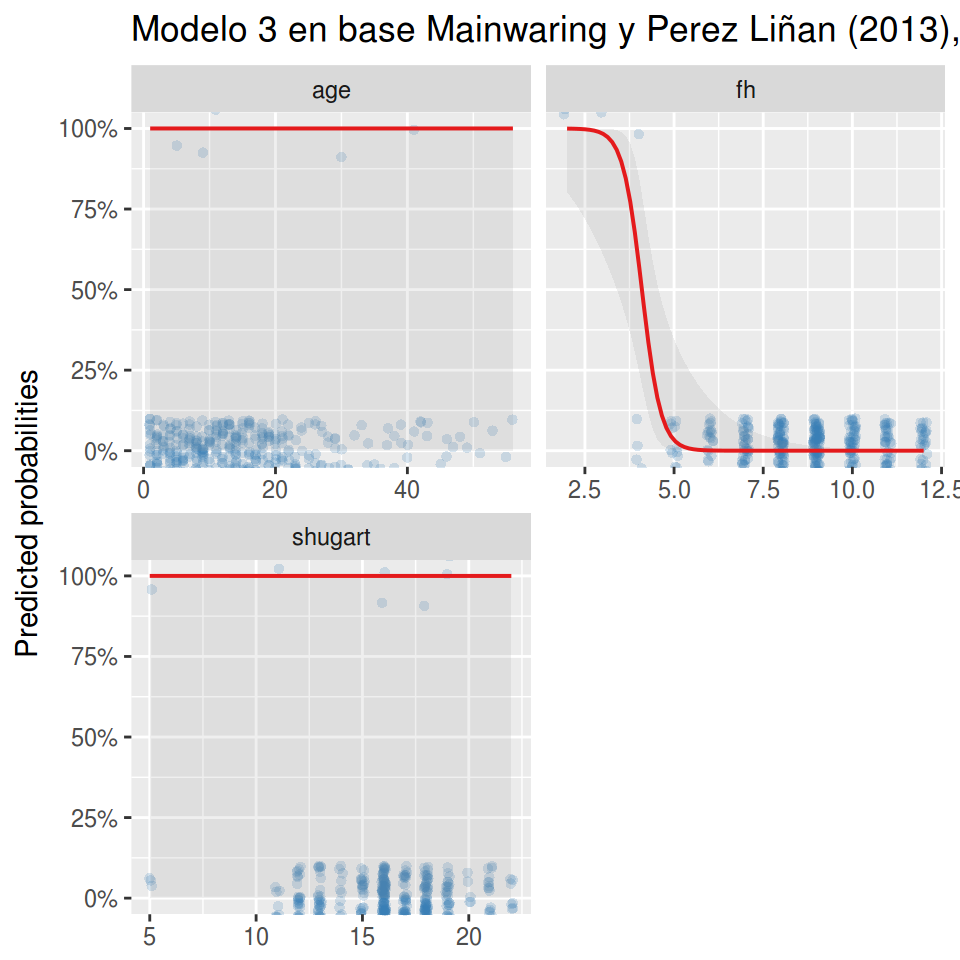
\includegraphics{adp-bookdown_files/figure-latex/unnamed-chunk-72-1} \end{center}

¿Qué especificamos?

\begin{enumerate}
\def\labelenumi{\arabic{enumi}.}
\tightlist
\item
  Primero, creamos una base de datos (``medias'') que contiene los
  promedios de ingresos por cada zona. Esto lo hicimos utilizando
  \texttt{group\_by} y \texttt{summarise} del \texttt{tidyverse}.
\end{enumerate}

\begin{Shaded}
\begin{Highlighting}[]
\NormalTok{datos_municipales }\OperatorTok\StringTok{ }
\StringTok{  }\KeywordTok{group_by}\NormalTok{(zona) }\OperatorTok\StringTok{ }
\StringTok{  }\KeywordTok{summarise}\NormalTok{(}\DataTypeTok{mean =} \KeywordTok{mean}\NormalTok{(ingresos, }\DataTypeTok{na.rm =}\NormalTok{ T))}
\CommentTok{## # A tibble: 5 x 2}
\CommentTok{##   zona             mean}
\CommentTok{##   <fct>           <dbl>}
\CommentTok{## 1 Norte Chico  4816249.}
\CommentTok{## 2 Norte Grande 7167984.}
\CommentTok{## 3 Zona Austral 2609648.}
\CommentTok{## 4 Zona Central 7302625.}
\CommentTok{## 5 Zona Sur     3219110.}
\end{Highlighting}
\end{Shaded}

\begin{enumerate}
\def\labelenumi{\arabic{enumi}.}
\setcounter{enumi}{1}
\item
  Especificamos el color de \texttt{geom\_line}.
\item
  Agregamos a nuestro código \texttt{geom\_hline}. Este objeto
  geométrico, como \texttt{geom\_vline} o \texttt{geom\_abline}, nos
  sirven para agregar líneas con información. En este caso, lo usé para
  agregar el promedio de ingresos de cada zona. Especificamos la
  variable que contiene los promedios \texttt{yintercept\ =\ mean}, de
  la base \texttt{medias}, y además, especificamos el color con
  \texttt{color\ =\ "dodgerblue3"}.
\item
  Usamos \texttt{scale\_x\_discrete} para especificar la expansión de
  los paneles. Si antes se veía un espacio gris sin información, lo
  sacaremos. Esto es estético.
\item
  Utilizamos \texttt{scale\_y\_log10} para escalar nuestros datos. Como
  los presentábamos, no lográbamos ver más allá de aquellos municipios
  con un altísimo ingreso, mientras que las demás comunas quedaban
  apiladas en el fondo del panel. Esta es una transformación logarítmica
  que normalmente se hace cuando trabajamos modelos lineales que
  contienen datos monetarios. Además, cambiamos las etiquetas del eje y:
  ya no aparece la notación científica. Esto se hace con un paquete
  llamado \texttt{scales}. Aquí llamamos directamente la función con
  \texttt{scales::dollar}.
\item
  Agregamos el título y los nombres del eje x y eje y con \texttt{labs}.
\item
  Especificamos información del tema. Sin él, los años entre un panel y
  otro chocarían. Para eso, especificamos con
  \texttt{panel.spacing\ =\ unit(2,\ "lines")} en la capa
  \texttt{theme}.
\end{enumerate}

Ejercicio:

\begin{itemize}
\tightlist
\item
  Para entender cómo funciona cada una de las especificaciones, puedes
  ir borrando y agregando por separado cada uno de estos detalles.
  Algunos tienen más sentido que otros, ¿qué modificarías?
\end{itemize}

\hypertarget{boxplot}{%
\subsection{Boxplot}\label{boxplot}}

Ya vimos que los ingresos de los municipios crecieron entre el 2004 y el
2012. Cuando observamos el gráfico sin la transformación funcional,
notamos que habían algunas comunas que tenían ingresos muy por sobre el
resto y sobresalían dentro de sus zonas. La intuición nos dice que
posiblemente sean \emph{outliers}. Podríamos ver esto más claramente con
un boxplot, el cual nos sirve para graficar diferentes datos
descriptivos de nuestras variables como son la mediana, el mínimo y el
máximo. En este caso, lo utilizaremos para ver si nuestra intuición era
acertada o no.

Filtramos los datos como lo hicimos con el gráfico anterior. En nuestro
eje x pondremos las zonas de Chile y en el eje y los ingresos. Además,
ocuparemos otro tipo de estética: \texttt{color}, la cual usaremos para
identificar de mejor manera cada zona. Propiedades estéticas como
\texttt{fill}, \texttt{color}, \texttt{size}, cambian al ser utilizadas
con variables discretas o continuas.

Este es el resultado que trabajaremos:

\begin{Shaded}
\begin{Highlighting}[]
\NormalTok{plot_c <-}\StringTok{ }\KeywordTok{ggplot}\NormalTok{(}\DataTypeTok{data    =}\NormalTok{ datos_municipales }\OperatorTok\StringTok{ }
\StringTok{                   }\KeywordTok{filter}\NormalTok{(year }\OperatorTok\StringTok{ }\KeywordTok{c}\NormalTok{(}\DecValTok{2004}\NormalTok{, }\DecValTok{2008}\NormalTok{, }\DecValTok{2012}\NormalTok{)),}
                 \DataTypeTok{mapping =} \KeywordTok{aes}\NormalTok{(}\DataTypeTok{x =}\NormalTok{ zona, }\DataTypeTok{y =}\NormalTok{ ingresos, }\DataTypeTok{color =}\NormalTok{ zona)) }\OperatorTok{+}
\StringTok{  }\KeywordTok{geom_boxplot}\NormalTok{() }\OperatorTok{+}
\StringTok{  }\KeywordTok{facet_wrap}\NormalTok{(}\OperatorTok{~}\NormalTok{year, }\DataTypeTok{ncol =} \DecValTok{1}\NormalTok{)}

\NormalTok{plot_c}
\end{Highlighting}
\end{Shaded}

\begin{center}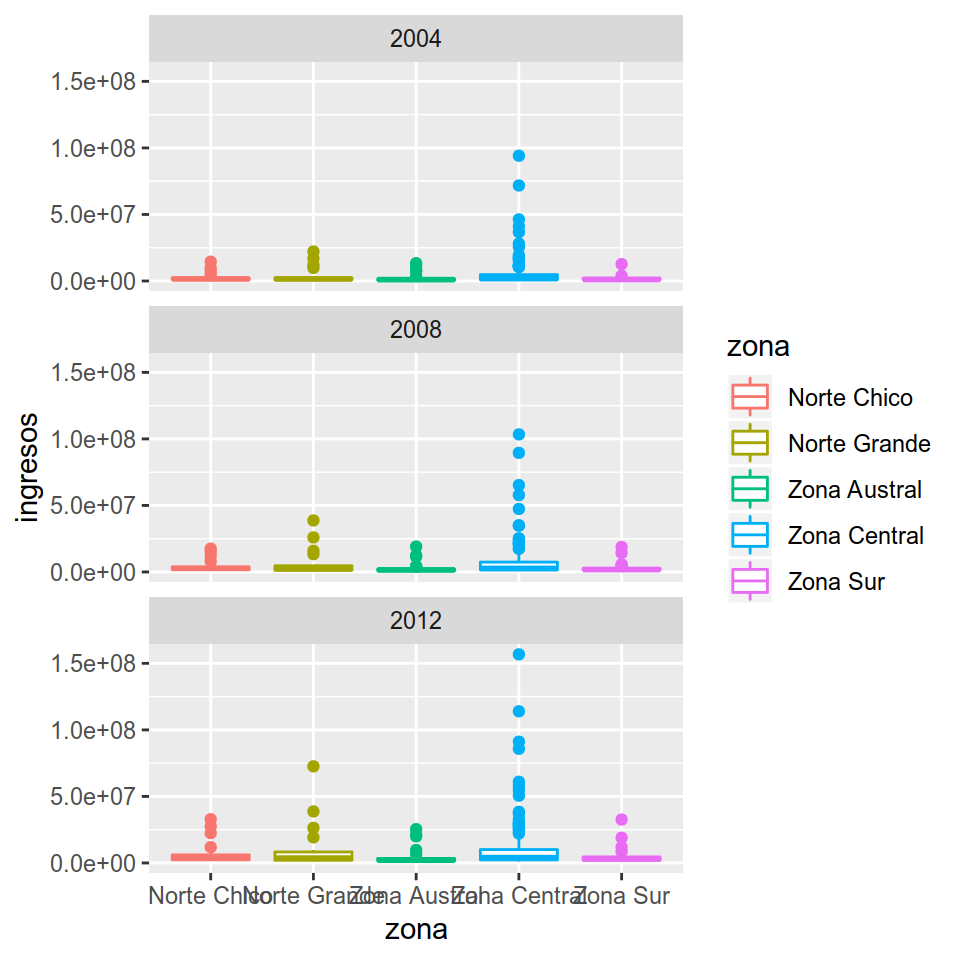
\includegraphics{adp-bookdown_files/figure-latex/unnamed-chunk-74-1} \end{center}

Uno de los problemas que podríamos tener con este gráfico, es que no nos
permite observar bien los outliers, ya que la expansión del eje y es muy
pequeña. Para solucionar esto podemos usar \texttt{coord\_flip}, una
función que nos permite dar vuelta los ejes de nuestro gráfico:

\begin{Shaded}
\begin{Highlighting}[]
\NormalTok{plot_c }\OperatorTok{+}\StringTok{ }
\StringTok{  }\KeywordTok{coord_flip}\NormalTok{() }
\end{Highlighting}
\end{Shaded}

\begin{center}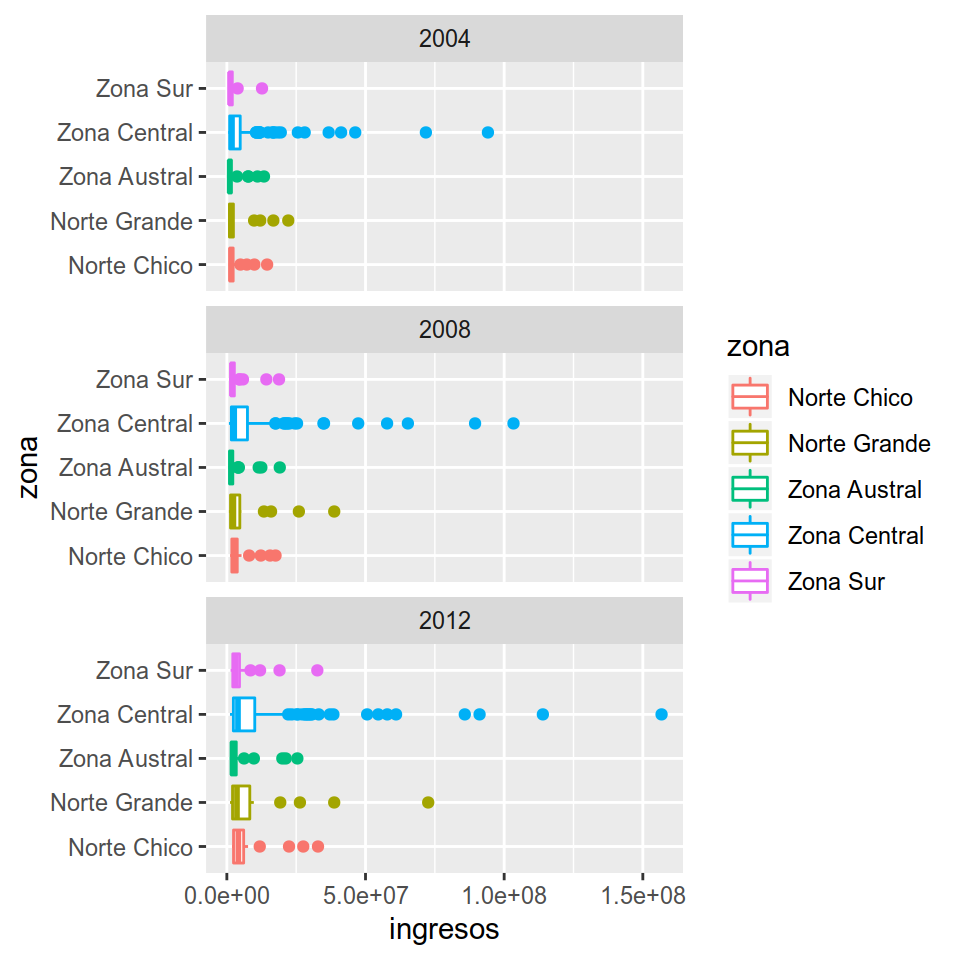
\includegraphics{adp-bookdown_files/figure-latex/unnamed-chunk-75-1} \end{center}

Ahora ya podemos observar mejor algunos de los \emph{outliers}
presentes. Quizás, después de ver estos resultados, nos gustaría
identificar qué comunas son las que reciben más ingresos totales. Para
eso podemos usar otra estética, \texttt{label} dentro de
\texttt{geom\_text}. Para nombrar sólo los outliers, tenemos que hacer
un subset de los datos.

\begin{Shaded}
\begin{Highlighting}[]
\NormalTok{plot_c }\OperatorTok{+}\StringTok{ }
\StringTok{  }\KeywordTok{coord_flip}\NormalTok{() }\OperatorTok{+}
\StringTok{  }\KeywordTok{geom_text}\NormalTok{(}\DataTypeTok{data    =}\NormalTok{ datos_municipales }\OperatorTok\StringTok{ }\KeywordTok{filter}\NormalTok{(ingresos }\OperatorTok{>}\StringTok{ }\DecValTok{50000000}\NormalTok{),}
            \DataTypeTok{mapping =} \KeywordTok{aes}\NormalTok{(}\DataTypeTok{label =}\NormalTok{ comuna))}
\end{Highlighting}
\end{Shaded}

\begin{center}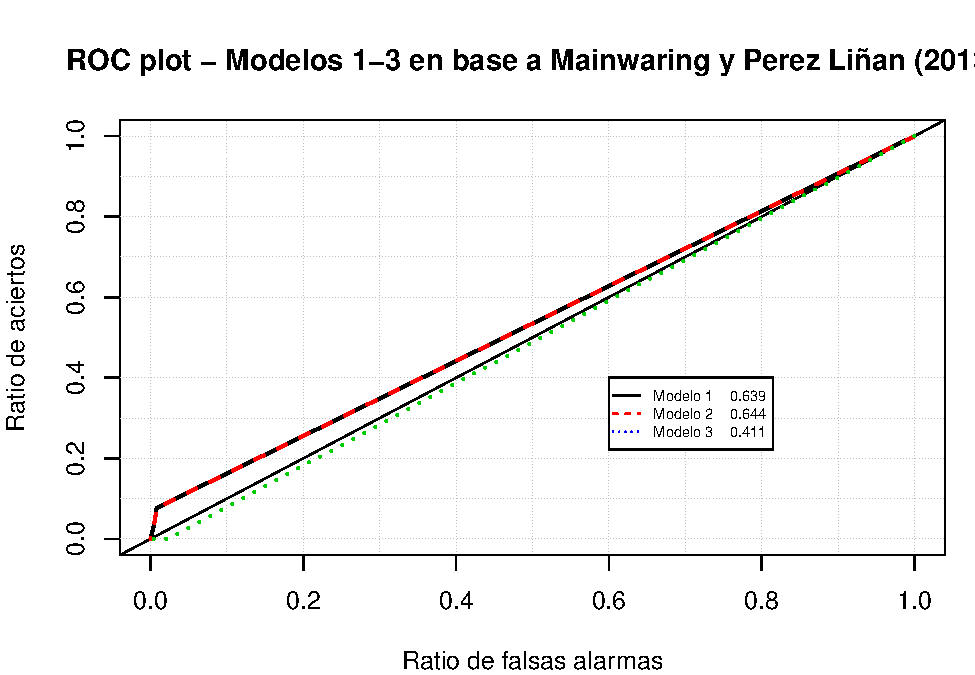
\includegraphics{adp-bookdown_files/figure-latex/unnamed-chunk-76-1} \end{center}

Lamentablemente, las etiquetas están por encima de los puntos y, en
algunos casos, se pierden cuando estos están muy juntos. Una de las
soluciones es con el paquete \texttt{ggrepel} que tiene el elemento
geométrico \texttt{geom\_text} ``mejorado'' para que las etiquetas no
choquen entre sí. También, cambiaremos el color de las letras para que
sea posible leerlas sin mayor dificultad. Como ven, este \texttt{color}
va afuera de la estética de \texttt{geom\_text\_repel}, ya que definimos
el color para todo el objeto. Cuando va dentro de \texttt{aes()}, el
color se modifica según la candidad de, por ejemplo, ingresos o por el
tipo de, por ejemplo, zona.

\begin{Shaded}
\begin{Highlighting}[]
\KeywordTok{library}\NormalTok{(ggrepel)}

\NormalTok{plot_c }\OperatorTok{+}\StringTok{ }
\StringTok{  }\KeywordTok{coord_flip}\NormalTok{() }\OperatorTok{+}
\StringTok{  }\KeywordTok{geom_text_repel}\NormalTok{(}\DataTypeTok{data    =}\NormalTok{ datos_municipales }\OperatorTok\StringTok{ }
\StringTok{                    }\KeywordTok{filter}\NormalTok{(ingresos }\OperatorTok{>}\StringTok{ }\DecValTok{50000000}\NormalTok{),}
                  \DataTypeTok{mapping =} \KeywordTok{aes}\NormalTok{(}\DataTypeTok{label =}\NormalTok{ comuna), }\DataTypeTok{color =} \StringTok{"black"}\NormalTok{)}
\end{Highlighting}
\end{Shaded}

\begin{center}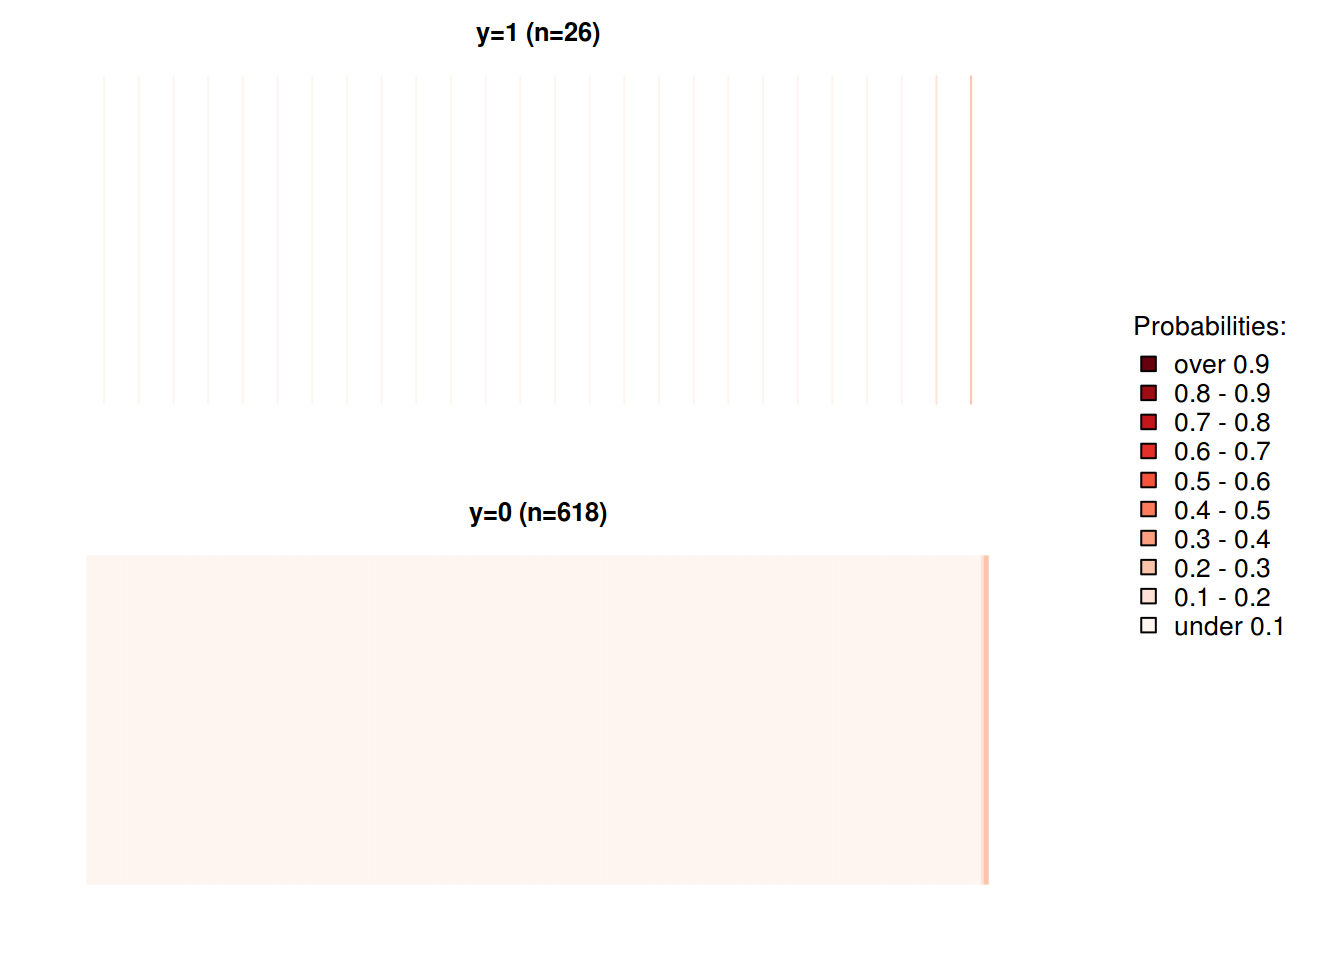
\includegraphics{adp-bookdown_files/figure-latex/unnamed-chunk-77-1} \end{center}

El corte puede ser en los \$50.000.000 o en números más grandes o más
pequeños. Depende completamente de lo que queremos observar. Además, con
\texttt{geom\_text} o \texttt{geom\_text\_repel} no solo puedes
modificar el color, sino también el el tipo de fuente de la letra, o si
debe estar en negrita, cursiva o subrayada. Para ver más opciones, debes
ingresar \texttt{?geom\_text} o llamar a \texttt{help("geom\_text")}.

También podríamos agregar otro tipo de información o cambiar cómo está
presentado lo que ya tenemos.

\begin{Shaded}
\begin{Highlighting}[]
\NormalTok{plot_c }\OperatorTok{+}\StringTok{ }
\StringTok{  }\KeywordTok{coord_flip}\NormalTok{() }\OperatorTok{+}
\StringTok{  }\KeywordTok{geom_text_repel}\NormalTok{(}\DataTypeTok{data =}\NormalTok{ datos_municipales }\OperatorTok\StringTok{ }
\StringTok{                    }\KeywordTok{filter}\NormalTok{(ingresos }\OperatorTok{>}\StringTok{ }\DecValTok{50000000}\NormalTok{), }
                  \DataTypeTok{mapping =} \KeywordTok{aes}\NormalTok{(}\DataTypeTok{label =}\NormalTok{ comuna), }
                  \DataTypeTok{color   =} \StringTok{"black"}\NormalTok{, }
                  \DataTypeTok{size    =} \DecValTok{3}\NormalTok{) }\OperatorTok{+}
\StringTok{  }\KeywordTok{scale_y_continuous}\NormalTok{(}\DataTypeTok{labels =}\NormalTok{ scales}\OperatorTok{::}\NormalTok{dollar) }\OperatorTok{+}
\StringTok{  }\KeywordTok{labs}\NormalTok{(}\DataTypeTok{title =} \StringTok{"Ingresos de las municipalidades según zona (2004-2012)"}\NormalTok{,}
       \DataTypeTok{x =} \StringTok{"Ingresos"}\NormalTok{, }\DataTypeTok{y =} \StringTok{"Zona"}\NormalTok{, }
       \DataTypeTok{caption =} \StringTok{"Fuente: Elaboración propia en base a datos del SINIM (2018)"}\NormalTok{) }\OperatorTok{+}
\StringTok{  }\KeywordTok{guides}\NormalTok{(}\DataTypeTok{color =}\NormalTok{ F)}
\end{Highlighting}
\end{Shaded}

\begin{center}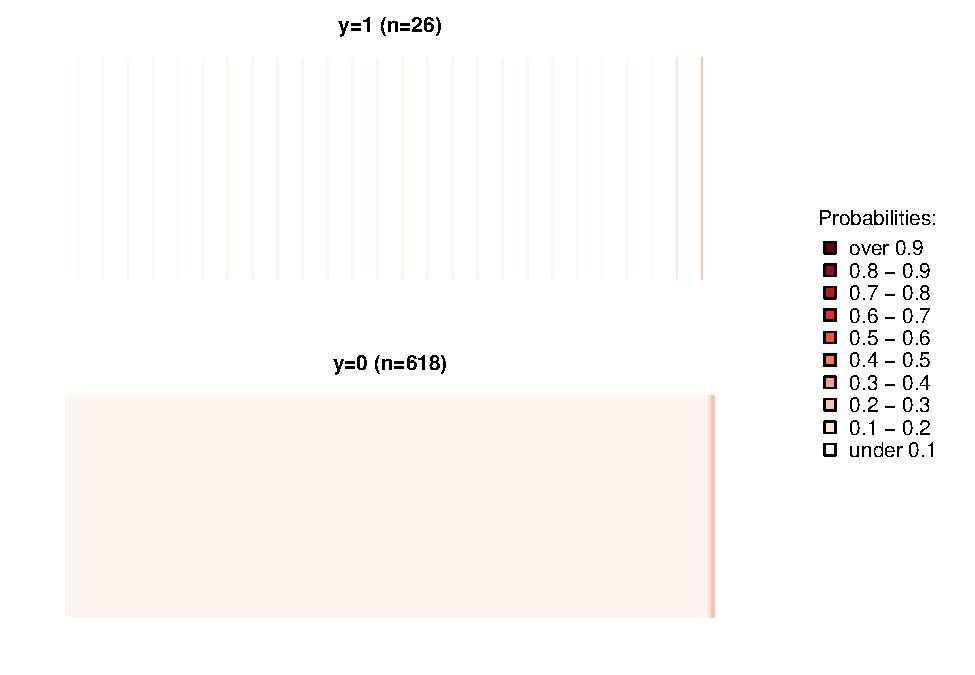
\includegraphics{adp-bookdown_files/figure-latex/unnamed-chunk-78-1} \end{center}

Otras especificaciones:

\begin{enumerate}
\def\labelenumi{\arabic{enumi}.}
\item
  Agregamos los nombres para los ejes y para el gráfico, además de la
  fuente de los datos.
\item
  Cambiamos el tamaño de la letra. Esto era importante por la cantidad
  de comunas que están por sobre los \$50.000.000 en ingresos.
\item
  Nuevamente, cambiamos las etiquetas del eje y con
  \texttt{scales::dollar}.
\item
  Por último, con \texttt{guides} y especificando el \texttt{aes()} que
  buscamos afectar, escribimos el código \texttt{color\ =\ F} para
  eliminar la leyenda, ya que era información que se repetía dentro del
  gráfico que realizamos.
\end{enumerate}

Te invito a jugar con \texttt{geom\_text}: cambia los colores, el
tamaño, la fuente, etc. También, te insto a instalar paquetes que te
permitirán personalizar aun más tus gráficos: \texttt{ggthemes} de
\href{https://github.com/jrnold/ggthemes}{jrnorl} tiene temas para
gráficos de programas y revistas conocidas como Excel o The Economist.
Por otro lado, \texttt{hrbrthemes} de
\href{https://github.com/hrbrmstr/hrbrthemes}{hrbrmstr} ha elaborado
algunos temas minimalistas y elegantes que harán que todos los gráficos
que hagas luzcan mejor. Si tienes algo por los colores, puedes mirar el
paquete \texttt{wespalette} de
\href{https://github.com/karthik/wesanderson}{karthik} una paleta
cromática basada en las películas de Wes Anderson o crear tus propias
paletas según imágenes con \texttt{colorfindr}. Puedes averiguar más
sobre este último en el siguiente
\href{https://github.com/zumbov2/colorfindr}{vínculo}.

\#\#\#Histograma

Según lo que pudimos observar en nuestro boxplot, muchas comunas
--especialmente de la zona central--, están muy por encima de los
ingresos medianos por zona. Podríamos ver la distribución de estos datos
a través de un histograma. Hacer un histograma es muy fácil, y como lo
había mencionado anteriormente, \texttt{geom\_histogram} no lleva el eje
y de forma explícita ya que cuenta la frecuencia de un evento dentro de
cierto intervalo.

Cuando creamos el histograma según nuestra intuición, este es el
resultado:

\begin{Shaded}
\begin{Highlighting}[]
\KeywordTok{ggplot}\NormalTok{(}\DataTypeTok{data    =}\NormalTok{ datos_municipales, }
       \DataTypeTok{mapping =} \KeywordTok{aes}\NormalTok{(}\DataTypeTok{x =}\NormalTok{ ingresos)) }\OperatorTok{+}
\StringTok{  }\KeywordTok{geom_histogram}\NormalTok{()}
\CommentTok{## `stat_bin()` using `bins = 30`. Pick better value with `binwidth`.}
\CommentTok{## Warning: Removed 738 rows containing non-finite values (stat_bin).}
\end{Highlighting}
\end{Shaded}

\begin{center}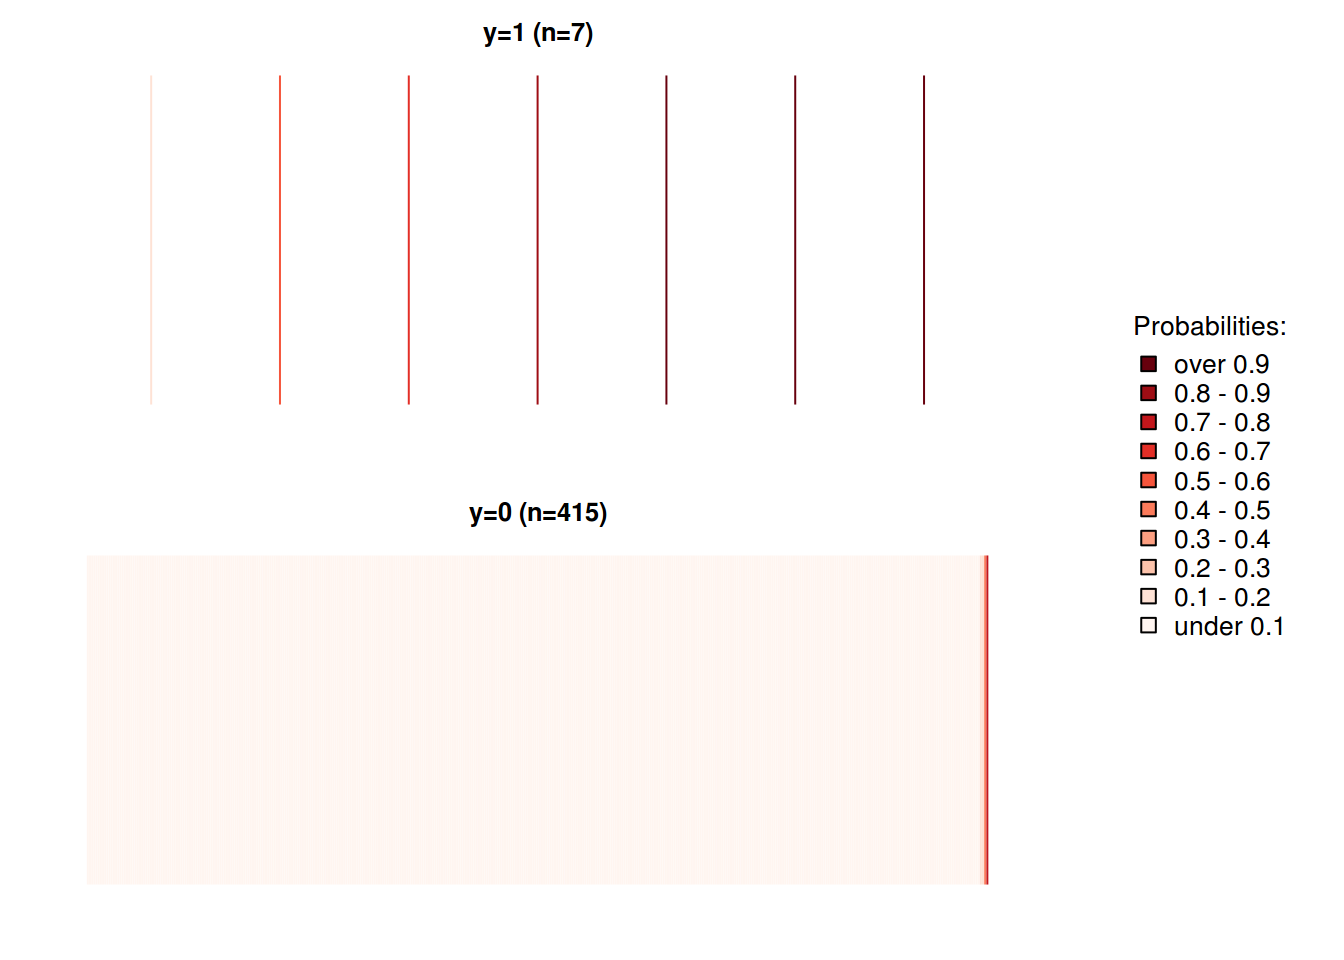
\includegraphics{adp-bookdown_files/figure-latex/unnamed-chunk-79-1} \end{center}

Como podemos observar, el gráfico nos tira un ``Warning'' que nos indica
que hay ``738 filas que contienen valores no-finitos''. Esta advertencia
se ha repetido constantemente durante el capítulo, y no quiere decir
nada más que ``Hay valores 0 o desconocidos dentro de esta variable'' y,
como sabemos, los primeros periodos no cuentan con información. Así que
tranquilo, si filtráramos los datos con
\texttt{filter(!is.na(ingresos))} lo más seguro es que la advertencia
desaparecería.

También, la consola nos dice este mensaje: \emph{\texttt{stat\_bin()}
using \texttt{bins\ =\ 30}. Pick better value with \texttt{binwidth}}.
Simplemente, nos dice que es posible modificar el número de intervalos.

Lo siguiente que haré será modificar el eje x. Nunca se me ha dado bien
leer los números con la notación científica. Por otro lado, probaremos
cambiando el número de intervalos con \texttt{bins}.

\begin{Shaded}
\begin{Highlighting}[]
\KeywordTok{ggplot}\NormalTok{(}\DataTypeTok{data    =}\NormalTok{ datos_municipales, }
       \DataTypeTok{mapping =} \KeywordTok{aes}\NormalTok{(}\DataTypeTok{x =}\NormalTok{ ingresos)) }\OperatorTok{+}
\StringTok{  }\KeywordTok{geom_histogram}\NormalTok{(}\DataTypeTok{bins =} \DecValTok{50}\NormalTok{) }\OperatorTok{+}
\StringTok{  }\KeywordTok{scale_x_continuous}\NormalTok{(}\DataTypeTok{labels =}\NormalTok{ scales}\OperatorTok{::}\NormalTok{dollar) }
\CommentTok{## Warning: Removed 738 rows containing non-finite values (stat_bin).}
\end{Highlighting}
\end{Shaded}

\begin{center}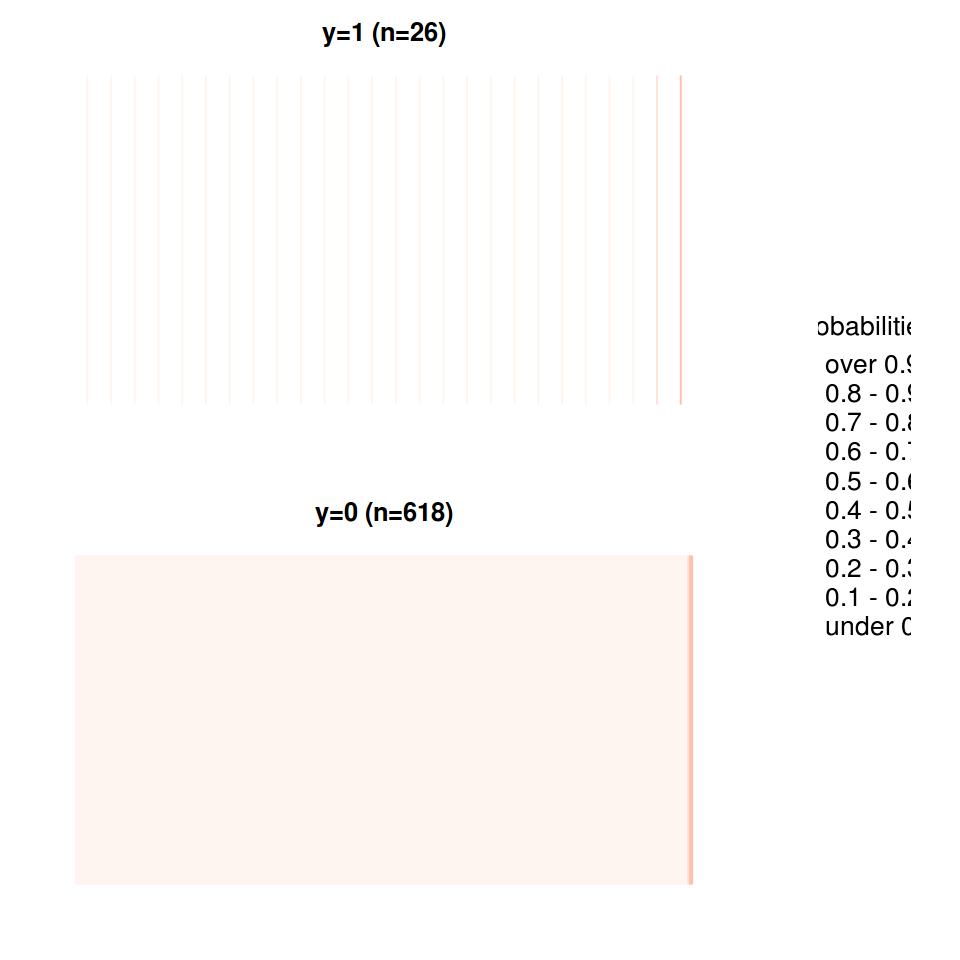
\includegraphics{adp-bookdown_files/figure-latex/unnamed-chunk-80-1} \end{center}

¿Qué pasa cuando ponemos \texttt{bins\ =\ 15} intervalos?

Lo que haremos a continuación es hacer un subset de los datos. Teniendo
en consideración el número de outliers que nos encontramos, eliminaremos
los municipios que tienen ingresos mayores a los \$50.000.000. También
podemos ver la frecuencia por zona. Al igual que cuando ocupamos
\texttt{color} con \texttt{geom\_boxplot}, ocuparemos \texttt{fill} con
\texttt{geom\_histogram}.

\begin{Shaded}
\begin{Highlighting}[]
\KeywordTok{ggplot}\NormalTok{(}\DataTypeTok{data    =}\NormalTok{ datos_municipales }\OperatorTok\StringTok{ }\KeywordTok{filter}\NormalTok{(ingresos }\OperatorTok{>}\StringTok{ }\DecValTok{50000000}\NormalTok{), }
       \DataTypeTok{mapping =} \KeywordTok{aes}\NormalTok{(}\DataTypeTok{x =}\NormalTok{ ingresos, }\DataTypeTok{fill =}\NormalTok{ zona)) }\OperatorTok{+}
\StringTok{  }\KeywordTok{geom_histogram}\NormalTok{(}\DataTypeTok{alpha =} \FloatTok{0.5}\NormalTok{, }\DataTypeTok{bins =} \DecValTok{50}\NormalTok{) }\OperatorTok{+}
\StringTok{  }\KeywordTok{scale_x_continuous}\NormalTok{(}\DataTypeTok{labels =}\NormalTok{ scales}\OperatorTok{::}\NormalTok{dollar) }\OperatorTok{+}
\StringTok{  }\KeywordTok{labs}\NormalTok{(}\DataTypeTok{title =} \StringTok{"Número de municipalidades según sus ingresos anuales (2004-2012)"}\NormalTok{,}
       \DataTypeTok{x =} \StringTok{"Ingresos"}\NormalTok{, }\DataTypeTok{y =} \StringTok{"Número de municipios"}\NormalTok{, }
       \DataTypeTok{caption =} \StringTok{"Fuente: Elaboración propia en base a datos del SINIM (2018)"}\NormalTok{)}
\end{Highlighting}
\end{Shaded}

\begin{center}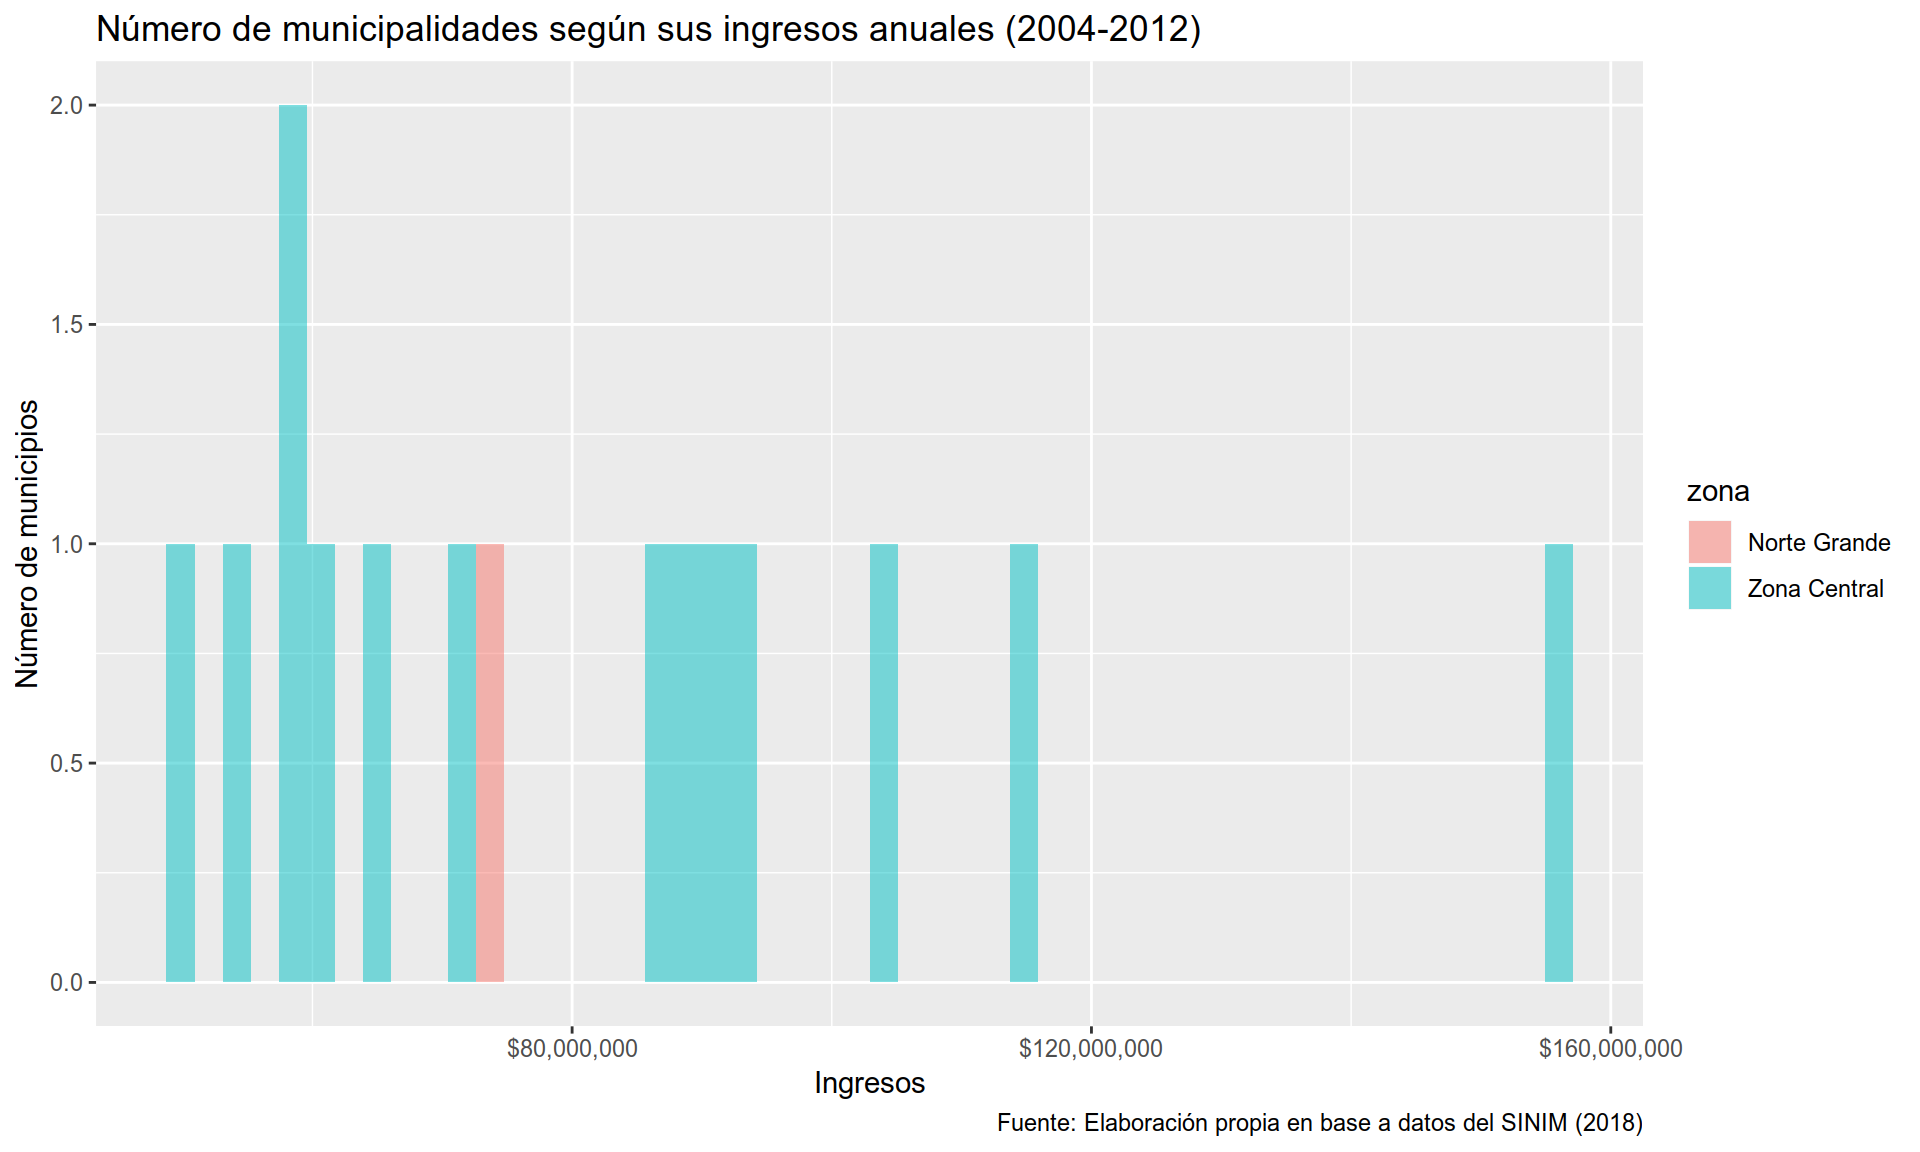
\includegraphics{adp-bookdown_files/figure-latex/unnamed-chunk-81-1} \end{center}

Ejercicio:

\begin{itemize}
\tightlist
\item
  La construcción de un gráfico de densidad es muy similar a la de un
  histograma, solo debes usar \texttt{geom\_density}. Teniendo los datos
  y la intuición, no debería ser complejo llegar a estos mismos
  resultados. Consejo: no solo uses \texttt{fill} para cambiar los
  colores, tambien usa \texttt{color}.
\end{itemize}

\hypertarget{relacion-entre-variables}{%
\subsection{Relación entre variables}\label{relacion-entre-variables}}

Probablemente una de tus mayores preocupaciones es si las dos variables
que estás estudiando se relacionan de algún modo. Con \texttt{ggplot}
esto es muy simple de comprobar. En este caso, tenemos dos variables
continuas: el porcentaje de pobreza de la CASEN y los ingresos
municipales. Según la teoría, debería existir un tipo de relación: a
mayor ingreso municipal, menor debería ser el porcentaje de pobreza en
la comuna. Creamos nuestros datos:

\begin{Shaded}
\begin{Highlighting}[]
\NormalTok{plot_f <-}\StringTok{ }\KeywordTok{ggplot}\NormalTok{(}\DataTypeTok{data    =}\NormalTok{ datos_municipales, }
                 \DataTypeTok{mapping =} \KeywordTok{aes}\NormalTok{(}\DataTypeTok{x =}\NormalTok{ casen, }\DataTypeTok{y =} \KeywordTok{log}\NormalTok{(ingresos)))}
\end{Highlighting}
\end{Shaded}

Para este tipo de gráfico, utilizamos \texttt{geom\_smooth}. Con este
objeto, puedes modificar la forma en que se relacionan las variables a
través de \texttt{method}. Incluso puedes poner tu propia fórmula. Por
defecto, viene especificada una relación lineal entre las variables, así
que no es necesario escribirlo.

\begin{Shaded}
\begin{Highlighting}[]
\NormalTok{plot_f }\OperatorTok{+}\StringTok{ }
\StringTok{  }\KeywordTok{geom_smooth}\NormalTok{(}\DataTypeTok{method =} \StringTok{"lm"}\NormalTok{, }\DataTypeTok{color =} \StringTok{"dodgerblue3"}\NormalTok{) }
\end{Highlighting}
\end{Shaded}

\begin{center}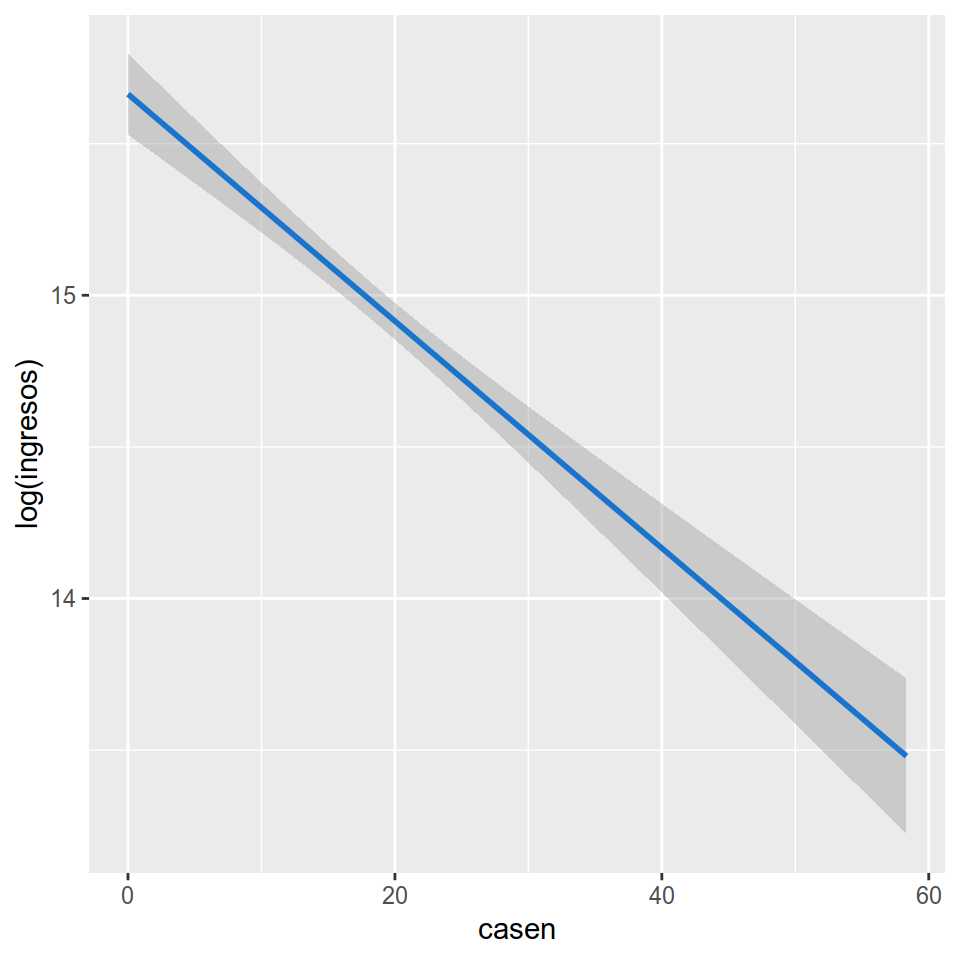
\includegraphics{adp-bookdown_files/figure-latex/unnamed-chunk-83-1} \end{center}

Se ve un poco vacío, ¿no? Normalmente, ocuparemos \texttt{geom\_smooth}
con otra figura geométrica \texttt{geom\_point}, para indicar la
posición de las comunas dentro del espacio. Ocuparemos \texttt{alpha}
para que veamos la sobreposición de los puntos. Sin ser muchos, no hay
problemas en ver cómo se distribuyen.

\begin{Shaded}
\begin{Highlighting}[]
\NormalTok{plot_f }\OperatorTok{+}\StringTok{ }
\StringTok{  }\KeywordTok{geom_point}\NormalTok{(}\DataTypeTok{alpha =} \FloatTok{0.3}\NormalTok{) }\OperatorTok{+}
\StringTok{  }\KeywordTok{geom_smooth}\NormalTok{(}\DataTypeTok{method =} \StringTok{"lm"}\NormalTok{, }\DataTypeTok{color =} \StringTok{"dodgerblue3"}\NormalTok{) }
\end{Highlighting}
\end{Shaded}

\begin{center}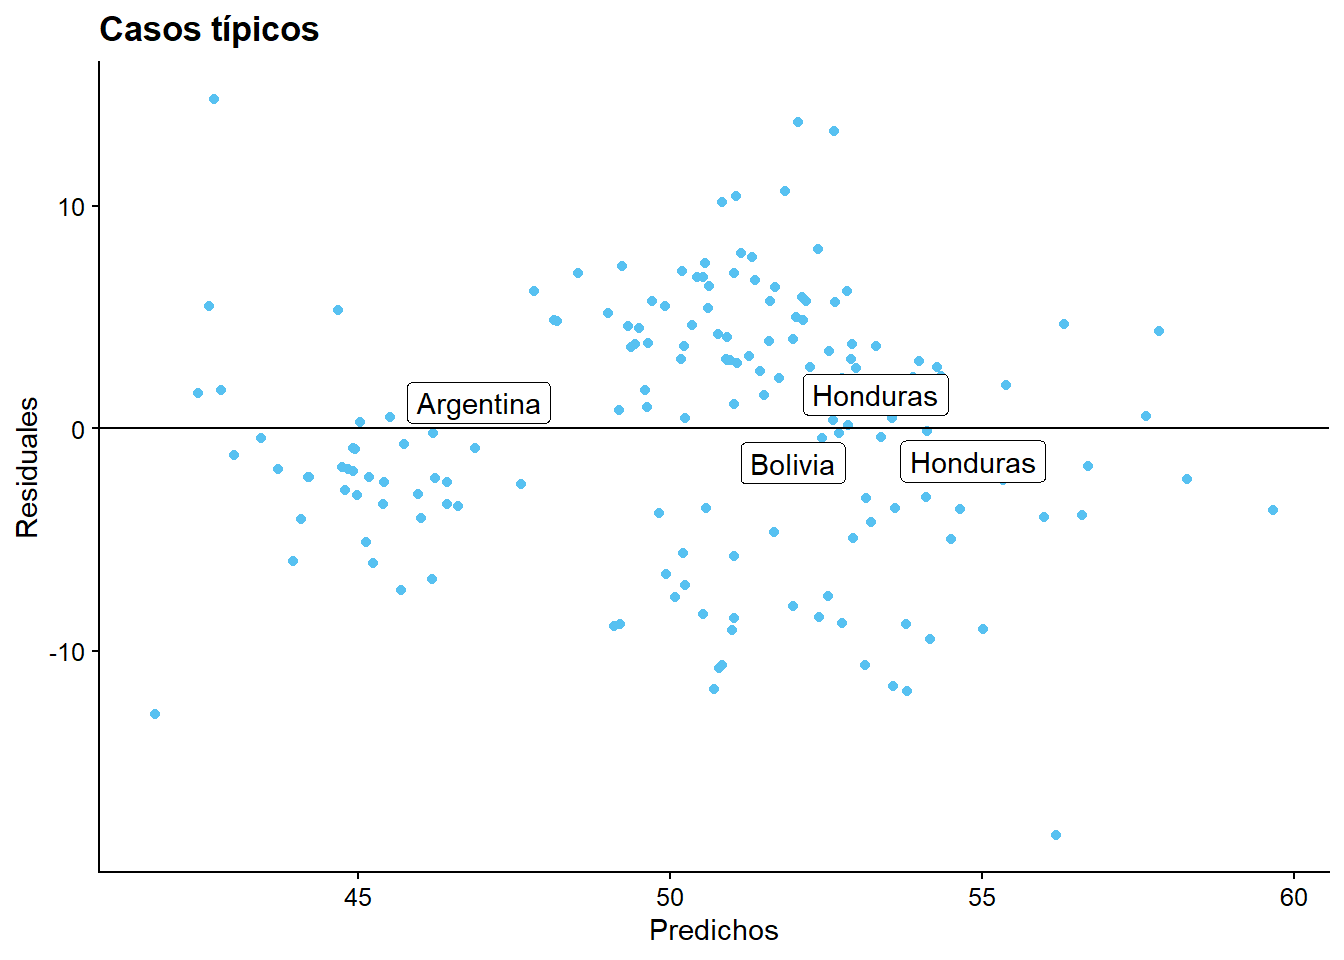
\includegraphics{adp-bookdown_files/figure-latex/unnamed-chunk-84-1} \end{center}

Ahora podríamos hacer dos especificaciones. Primero, pondremos el título
y el nombre de los ejes. Segundo, en \texttt{geom\_x\_continuous}
especificaremos donde tiene que empezar y terminar nuestro gráfico. Esto
ya lo habíamos usado con \texttt{geom\_line}.

\begin{Shaded}
\begin{Highlighting}[]
\NormalTok{plot_f }\OperatorTok{+}\StringTok{ }
\StringTok{  }\KeywordTok{geom_point}\NormalTok{(}\DataTypeTok{alpha =} \FloatTok{0.3}\NormalTok{) }\OperatorTok{+}
\StringTok{  }\KeywordTok{geom_smooth}\NormalTok{(}\DataTypeTok{method =} \StringTok{"lm"}\NormalTok{, }\DataTypeTok{color =} \StringTok{"dodgerblue3"}\NormalTok{) }\OperatorTok{+}
\StringTok{  }\KeywordTok{scale_x_continuous}\NormalTok{(}\DataTypeTok{expand =} \KeywordTok{c}\NormalTok{(}\DecValTok{0}\NormalTok{,}\DecValTok{0}\NormalTok{)) }\OperatorTok{+}
\StringTok{  }\KeywordTok{labs}\NormalTok{(}\DataTypeTok{title =} \StringTok{"Relación entre ingresos y porcentaje de pobreza CASEN, Chile (2004-2012)"}\NormalTok{, }
       \DataTypeTok{x =} \StringTok{"Porcentaje de Pobreza CASEN"}\NormalTok{, }\DataTypeTok{y =} \StringTok{"Ingresos"}\NormalTok{, }
       \DataTypeTok{caption =} \StringTok{"Fuente: Elaboración propia en base a datos del SINIM (2018)"}\NormalTok{) }
\end{Highlighting}
\end{Shaded}

\begin{center}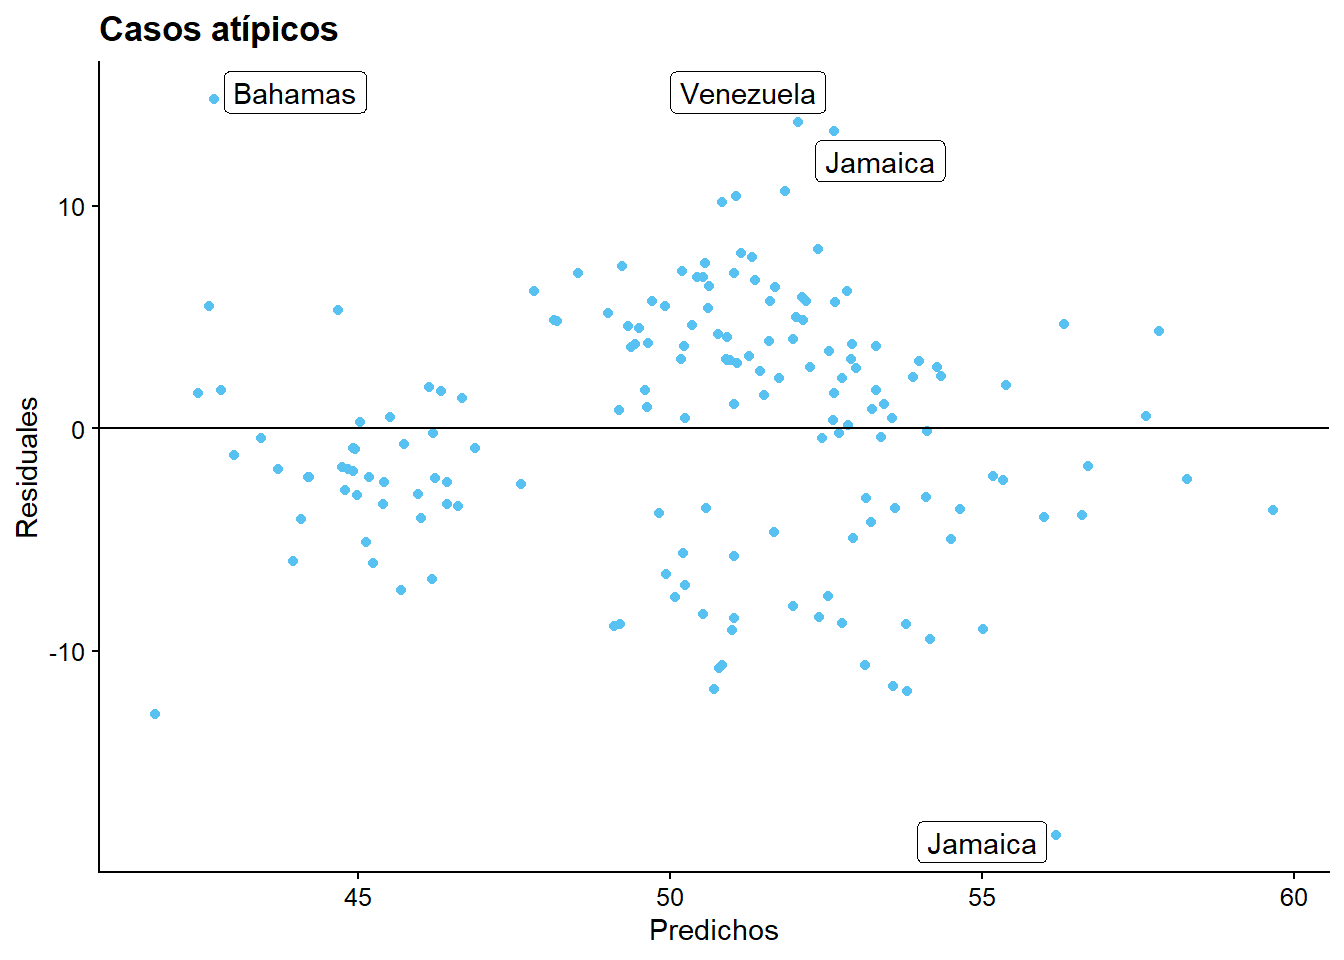
\includegraphics{adp-bookdown_files/figure-latex/unnamed-chunk-85-1} \end{center}

Claramente, hay una correlación negativa entre ambas variables. Era lo
que esperábamos. Ahora, podemos calcular la correlación entre ambas para
estar más seguros de los resultados obtenidos:

\begin{Shaded}
\begin{Highlighting}[]
\KeywordTok{cor}\NormalTok{(datos_municipales}\OperatorTok{$}\NormalTok{casen, datos_municipales}\OperatorTok{$}\NormalTok{ingresos, }
    \DataTypeTok{use =} \StringTok{"pairwise.complete.obs"}\NormalTok{)}
\CommentTok{## [1] -0.27}
\end{Highlighting}
\end{Shaded}

La correlación entre ambas variables es de -0.27. Sería interesante
agregar esta información al gráfico. Esto lo podemos realizar con
\texttt{annotate}. Sólo tenemos que especificar el tipo de objeto
geométrico que queremos generar. En este caso, lo que queremos crear es
texto \texttt{text}, pero podría ser un cuadro resaltando un punto
específico en el gráfico \texttt{rect} o una línea \texttt{segment}.
Especificamos donde lo ubicaremos y, finalmente, anotamos lo que
queremos anotar.

\begin{Shaded}
\begin{Highlighting}[]
\NormalTok{plot_f }\OperatorTok{+}\StringTok{ }
\StringTok{  }\KeywordTok{geom_point}\NormalTok{(}\DataTypeTok{alpha =} \FloatTok{0.3}\NormalTok{) }\OperatorTok{+}
\StringTok{  }\KeywordTok{geom_smooth}\NormalTok{(}\DataTypeTok{method =} \StringTok{"lm"}\NormalTok{, }\DataTypeTok{color =} \StringTok{"dodgerblue3"}\NormalTok{) }\OperatorTok{+}
\StringTok{  }\KeywordTok{scale_x_continuous}\NormalTok{(}\DataTypeTok{expand =} \KeywordTok{c}\NormalTok{(}\DecValTok{0}\NormalTok{,}\DecValTok{0}\NormalTok{)) }\OperatorTok{+}
\StringTok{  }\KeywordTok{labs}\NormalTok{(}\DataTypeTok{title =} \StringTok{"Relación entre ingresos y porcentaje de pobreza CASEN, Chile (2004-2012)"}\NormalTok{, }
       \DataTypeTok{x =} \StringTok{"Porcentaje de Pobreza CASEN"}\NormalTok{, }\DataTypeTok{y =} \StringTok{"Ingresos"}\NormalTok{, }
       \DataTypeTok{caption =} \StringTok{"Fuente: Elaboración propia en base a datos del SINIM (2018)"}\NormalTok{) }\OperatorTok{+}
\StringTok{  }\KeywordTok{annotate}\NormalTok{(}\StringTok{"text"}\NormalTok{, }\DataTypeTok{x =} \DecValTok{50}\NormalTok{, }\DataTypeTok{y =} \DecValTok{15}\NormalTok{, }\DataTypeTok{label =} \StringTok{"Correlación:}\CharTok{\textbackslash{}n}\StringTok{-0.27"}\NormalTok{)}
\end{Highlighting}
\end{Shaded}

\begin{center}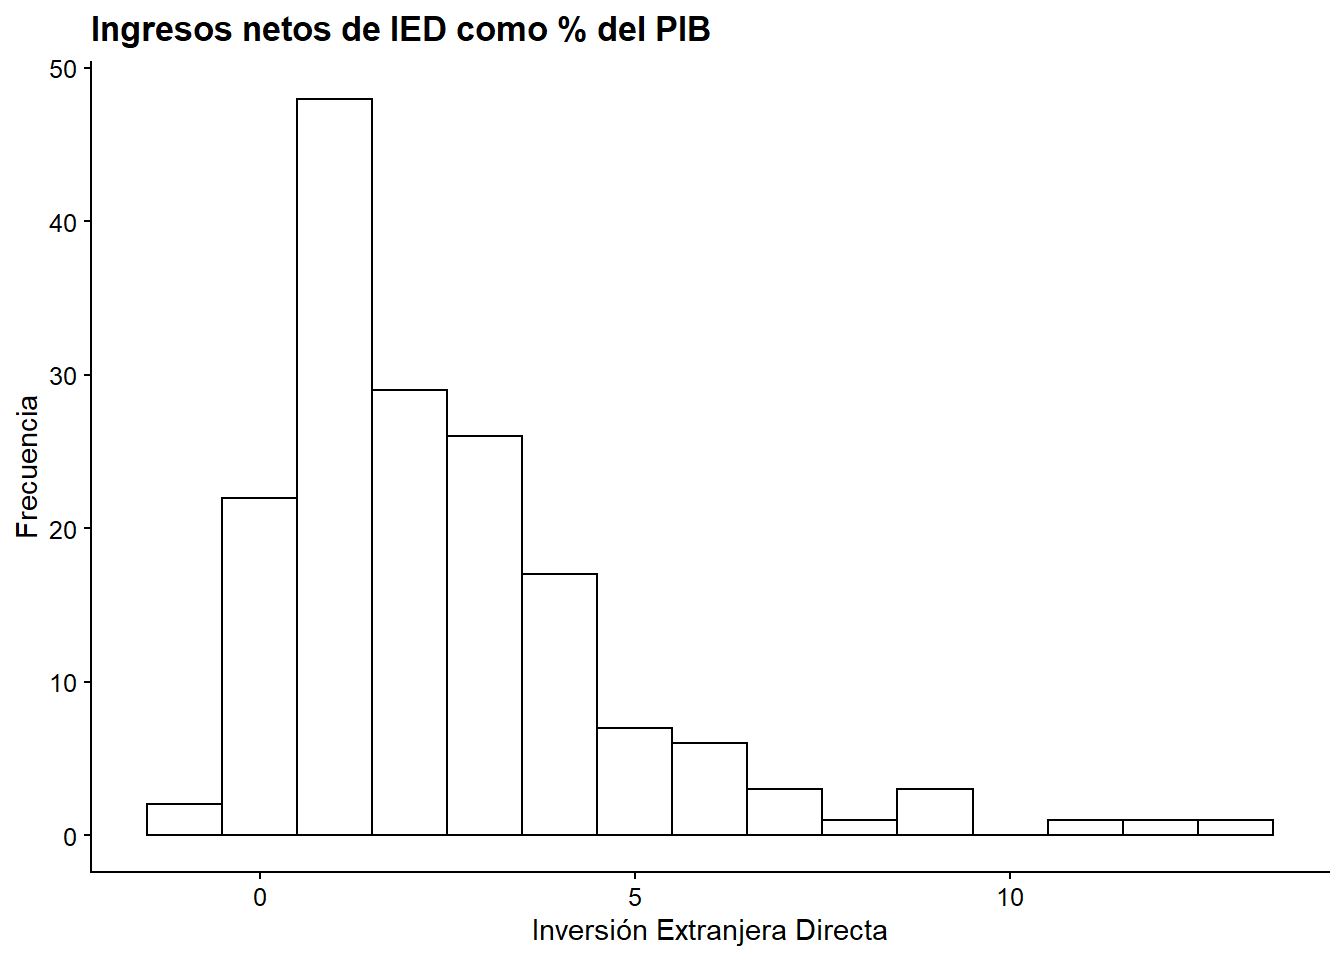
\includegraphics{adp-bookdown_files/figure-latex/unnamed-chunk-87-1} \end{center}

\hypertarget{para-seguir-aprendiendo}{%
\section{Para seguir aprendiendo}\label{para-seguir-aprendiendo}}

Para visualizar tus datos, hay diferentes caminos. En esta entrada,
pudiste conocer las principales funciones de \texttt{ggplot2} un paquete
del \texttt{tidyverse}, pero hay muchos paquetes que pueden ser de ayuda
en otro tipo de visualizaciones. Si bien \texttt{ggplot2} puede no tener
todas los obetos geométricos que necesites, hay otros paquetes para
visualizar otro tipo de datos que funcionan bajo \texttt{ggplot} y las
capas que componen esta forma ``gramatical''.

\hypertarget{otros-paquetes}{%
\subsection{Otros paquetes:}\label{otros-paquetes}}

\#\#\#\#\texttt{sf}

(vincular con capítulo de Andrea y Gabriel)

Permite visualizar elementos espaciales. Para \texttt{ggplot} actúa con
\texttt{geom\_sf}. Permite crear figuras geográficas con diferentes
tipos de datos espaciales. En el capítulo \_ sobre datos espaciales,
Andrea y Gabriel entregan las herramientas para trabajar con
\texttt{sf}, sus principales funciones y directrices.
\href{https://github.com/r-spatial/sf}{Aquí} puedes encontrar más
detalles sobre cómo instalarlo y su funcionamiento dependiento de tu
ordenador.

\hypertarget{ggparliament}{%
\subsubsection{\texorpdfstring{\texttt{ggparliament}}{ggparliament}}\label{ggparliament}}

Probablemente, todos los cientistas políticos deberíamos conocer este
paquete. Este paquete permite hacer visualizaciones con la composición
del poder legislativo. Soñado para quién trabaja con ese tipo de
información. Te permite especificar el número de escaños, el color de
cada uno de los partidos, y añadir diferentes características a tus
gráficos. \href{https://github.com/RobWHickman/ggparliament}{Aquí}
puedes encontrar más detalles sobre las herramientas de
\texttt{ggparliament}.

\hypertarget{ggraph}{%
\subsubsection{\texorpdfstring{\texttt{ggraph}}{ggraph}}\label{ggraph}}

Si estudias redes y conoces el funcionamiento de \texttt{ggplot2}, este
paquete puede convertirse en tu nuevo mejor amigo. Está hecho para todo
tipo de datos relacionales, y si bien funciona con la lógica de
\texttt{ggplot2}, tiene su propio conjunto de objetos geométricos,
\emph{facets}, entre otros.
\href{https://github.com/thomasp85/ggraph}{Aquí} puedes encontrar más
información.

\hypertarget{part-modelos}{%
\part{Modelos}\label{part-modelos}}

\hypertarget{logit}{%
\chapter{Modelos binarios}\label{logit}}

\hypertarget{surv}{%
\chapter{Modelos de supervivencia}\label{surv}}

Hay una serie de preguntas recurrentes al análisis de datos políticos
que aún no hemos cubierto. Muchas veces nos interesa saber por qué
ciertos eventos duran lo que duran, o porqué algunas observaciones duran
más que otras. ¿Por qué la paz es tan duradera entre algunos países
mientras que otros guerrean con frecuencia? ¿Cuál es la probabilidad de
que Turquía ingrese a la ingresar a la Unión Europea en 2018? ¿Por qué
algunos legisladores permanecen en sus cargos por varios periodos
consecutivos mientras que otros no logran reelegirse tan solo una vez?
¿Cuánto demora un sindicato en entrar en huelga durante una crisis
económica?

Todas estas preguntas tienen en común que la duración y el momento de
ocurrencia de un evento son parte de la respuesta que buscamos.
Necesitamos un modelo que nos permita llegar a esta respuesta. Janet
Box-Steffensmeier, la principal referencia en Ciencia Política de este
método, se refiere a ellos a ``modelos de eventos históricos'' aunque
buena parte de la literatura los llama modelos de supervivencia o
modelos de duración. Si bien en la Ciencia Política no son modelos tan
utilizados como uno creería (en el fondo, casi todas las preguntas que
nos hacemos pueden ser reformuladas en una pregunta sobre la duración
del evento), las ciencias médicas han explorado estos métodos en
profundidad, y muchas las referencias que uno encuentra en R sobre
paquetes accesorios a estos modelos son de departamentos bioestadísticos
y médicos. De allí que ``modelos de supervivencia'' sea el nombre más
frecuentemente utilizado para estos modelos, ya que en medicina comenzó
a utilizárselos para modelar qué variables afectaban la sobrevida de sus
pacientes enfermos.

Podemos tener dos tipos de bases de datos para estos problemas. Por un
lado podemos tener una base en formato de panel en el que para un
momento dado nuestra variable dependiente codifica si el evento ha
ocurrido (=1) o no (=0). Así, por ejemplo, podemos tener una muestra de
veinte países para cincuenta años (1965-2015) en los que nuestra
variable de interés es si el país ha implementado una reforma
constitucional. La variable independiente asumirá el valor 1 para el año
1994 en Argentina, pero será 0 para el resto de los años en este país.
Por otro lado, podemos tener una base de datos transversal en la que
cada observación aparece codificada apenas una vez. En este caso
necesitamos, además de la variable que nos dirá si en el periodo de
interés el evento ocurrió o no para cada observación (por ejemplo,
Argentina debería ser codificada como ``1''), una variable extra que
codifique el tiempo de ``supervivencia'' de cada observación, es decir,
cuánto tiempo pasó hasta que finalmente el evento sucedió. Para el caso
de Argentina, esta variable codificará 29 (años), que es lo que demoró
en implementarse una reforma constitucional desde 1965. La elección del
año de partida, como podrá sospechar, es decisión del investigador, pero
tiene un efecto enorme sobre nuestros resultados.

Supongamos que nos hacemos la pregunta que se hizo David Altman: ``¿Por
qué algunos países demoran menos que otros en implementar instancias de
democracia directa?''. Para ello tenemos una base de datos en formato de
panel que parte del año 1900 y que llega a 2016 para 202 países (algunas
observaciones, como la Unión Soviética se transforman en otras
observaciones a partir de un determinado año en que dejan de existir).
Al observar sus datos uno nota algo que probablemente también te suceda
en tu base de datos. Para el año 2016 apenas un pequeño porcentaje de
países había implementado este tipo de mecanismos (27\% para ser más
precisos) pero la base está censurada ya que a partir de ese año no
sabemos que ha ocurrido con los países que aún no han implementado
mecanismos de democracia directa. No todas las observaciones han
``muerto'' aún, ¿cómo saber cuándo lo harán? Ésta es una pregunta
válida, que podremos responder con este tipo de modelos, ya que podemos
calcular el tiempo que demorará cada uno de los países censurados en
nuestra muestra (con la información que le damos al modelo, que siempre
es incompleta).

En nuestra base de datos tendremos, al menos, tres tipos de
observaciones (ver figura x): (a) aquellas que, para el momento en que
tenemos datos ya estaban en la muestra, aunque no siempre sabremos hace
cuanto que ``existen'' (en la base de datos de Altman, por ejemplo,
México ya existía como entidad política en 1900, cuando su base de datos
parte. Sabemos que la Primera República Federal existió como entidad
política desde octubre de 1824, por lo que México sería codificado como
existente a partir de esa fecha). Lo que sí sabemos es que en 2012, por
primera vez, México implementó una iniciativa de democracia directa, lo
que define como positiva la ocurrencia del evento que nos interesa
medir; (b) Algunas observaciones estarán desde el comienzo de la
muestra, y existirán hasta el último momento sin haber registrado el
evento de interés. Tal es el caso, en la muestra de Altman, de Argentina
que ya en 1900 está registrado en la base, y hasta el último año de la
muestra no había registrado instancias de democracia directa, lo que la
transforma en una observación censurada; (c) Algunas observaciones
pueden entrar ``tarde'' en la muestra. Por ejemplo, Eslovenia entra a la
muestra de Altman en 1991, que es cuando se independiza de Yugoslavia.

Figura x. (*) hay que hacer un equivalente propio a esta figura.. en el
que el país 1 entre en t2 a la muestra y el país 4 en t5

(insertar fórmulas a continuación)

Los modelos de supervivencia se interpretan a partir de la probabilidad
de que en un momento dado el evento de interés ocurra dado que no ha
ocurrido aun. Esta probabilidad recibe el nombre de tasa de riesgo.
Partimos sabiendo que tenemos una variable, que llamaremos \(T\), y que
representa un valor aleatorio positivo y que tiene una distribución de
probabilidades (correspondiente a la probabilidad del evento ocurrir en
cada uno de los momentos posibles), que llamaremos \(f(t)\), y que se
puede expresar de manera acumulada, como una densidad acumulada
\(F(t)\). Como dijimos que \(T\) es una variable aleatoria, podemos
calcular su distribución que viene dada por la fórmula, en la que vemos
que \(F(t)\) viene dada por la probabilidad de que el tiempo de
supervivencia \(T\) sea menor o igual a un tiempo específico \(t\).

\(F(t)=\int\limits_0^t f(u)d(u)=Pr(T)\leq t)\)

La función de supervivencia \(\hat S(t)\), que es un concepto clave en
estos modelos, está relacionada a \(F(t)\), ya que

\(\hat S(t)= 1-F(t)=Pr(T\geq t)\)

Es decir, la función de supervivencia es la probabilidad inversa de
\(F(t)\), pues dice respecto a la probabilidad de que el tiempo de
supervivencia \(T\) sea mayor o igual un tiempo \(t\) de interés. Para
el ejemplo concreto de Altman, uno podría preguntarse cuál es la
probabilidad de un país no implementar un mecanismo de democracia
directa (lo que sería equivalente a ``sobrevivir'' a dicha
implementación) siendo que ya ha sobrevivido a los mismos por 30 años. A
medida que más y más países en la muestra van implementando iniciativas
de democracia directa, la probabilidad de supervivencia va disminuyendo.

Los coeficientes de los modelos de supervivencia se suelen interpretar
como tasas de riesgo (o ``hazard rates'' en inglés), que es el cociente
de la probabilidad de que el evento suceda y la función de supervivencia

\(h(t)=\frac{f(t)}{S(t)}\)

Así, la tasa de riesgo indica la tasa a la que las observaciones
``mueren'' en nuestra muestra en el momento \(t\), considerando que la
observación ha sobrevivido hasta el momento \(t\). Veremos más adelante
como en el ejemplo de Altman podemos interpretar los coeficientes de
nuestras regresiones como tasas de riesgo. En definitiva, la tasa de
riesgo \(h(t)\) es el riesgo de que el evento ocurra en un intervalo de
tiempo determinado, que viene dado por

\(f(t)=\lim_{\bigtriangleup x \to 0} \frac {P(t+\bigtriangleup t > T \geq t)}{\bigtriangleup t}\)

\hypertarget{el-modelo-cox-de-riesgos-proporcionales}{%
\section{El modelo Cox de riesgos
proporcionales:}\label{el-modelo-cox-de-riesgos-proporcionales}}

Hay dos tipos de modelos de supervivencia, los llamados modelos
paramétricos y los llamados semi-parametricos. Los primeros son aquellos
que hacen supuestos sobre las características de la población a la que
la muestra pertenece. En este caso, los supuestos son sobre el
``baseline hazard'', es decir, sobre el riesgo de que el evento ocurra
cuando todas nuestras variables independientes son iguales a cero. El
tipo de modelo de surpervivencia más común para esta categoría es el
modelo de Weibull. Por otro lado, los modelos semi-parametricos no hacen
ningún tipo de asunciones sobre la función de base, ya que ésta es
estimada a partir de los datos. El ejemplo más famoso de ésta
especificación es la del modelo de Cox.

El Oxford Handbook sobre metodología política dedica un capítulo entero
a discutir modelos de supervivencia, y en él se toma una posición fuerte
en favor de los modelos semi-parametricos. Por un lado, como no se hacen
presupustos sobre la función del riesgo de base, su estimación es mucho
más precisa. En una estimación paramétrica, elegir un ``baseline
hazard'' equivocado siginificará que todo nuestro trabajo analítico
estará sesgado. La decisión de la forma que adopta la curva de base en
un modelo de Weibull debería estar orientado por razones teóricas de
cuál es el efecto de nuestra variable independiente sobre la
probabilidad de supervivencia de la observación (ver figura x). Sin
embargo, no siempre hay tales presupuestos. Elegir una especificación
por Cox nos ahorra de tomar una decisión tan costosa.

Figura x. diferentes riesgos de base en el modelo de Weibull (dibujar
manualmente)

Una segunda ventaja de los modelos semi-parametricos sobre los
paramétricos tiene que ver con el presupuesto de riesgos proporcionales.
Ambos, modelos paramétricos y semi-parametricos asumen que los riesgos
entre dos individuos cualquiera de la muestra se mantienen constantes a
lo largo de todo su periodo de supervivencia. Es decir, se asume que la
curva de riesgo de cada individuo sigue la misma curva en el tiempo.
Ésta es una asunción cara para trabajos en ciencia política, en los que
las observaciones cambian en el tiempo y se diferencian unas de otras.
Piénsense en el trabajo de Altman, por ejemplo. Uno puede teorizar que
la probabilidad de una iniciativa de democracia directa suceder en el
tiempo estará afectada por el nivel de solidez de sus instituciones
democráticas, que podemos medir con algún tipo de variable estándar como
los 21 puntos de Polity IV o la más reciente medición de V-Dem. Podemos,
entonces, esperar que, a mayor solidez institucional, mayor probabilidad
de implementar mecanismos de democracia directa. Sin embargo los valores
de estas variables no solo difieren ente países, sino que a lo largo del
tiempo estas variables cambian mucho para un mismo país. Piénsese en
Colombia, por ejemplo, que en la variable de V-Dem ``v2x\_polyarchy''
sufrió avances y retrocesos entre 1900 y 2016. Cada vez que el valor de
esta variable cambia, necesariamente cambia la tasa de riesgo de
democracia directa para Colombia, rompiendo el presupuesto de
proporcionalidad de los riesgos (ver figura x).

Figura x. evolución en el tiempo de la variable de V-Dem
``v2x\_polyarchy'' para Colombia (hacer en R)

La ventaja del modelo de Cox sobre sus contrapartes paramétricas es que
existen tests para saber si alguna variable de nuestro modelo rompe el
presupuesto de proporcionalidad de los riesgos, y de esa forma podremos
corregirlo generando interacciones entre estas variables y variables
temporales. De esta forma, permitimos que en nuestro modelo haya dos
tipos de coeficientes: coeficientes constantes en el tiempo, y
coeficientes cambiantes en el tiempo. Por ejemplo, podemos imaginar que
ante un aumento brusco en la calidad de las instituciones democráticas
de un país la tasa de riesgo de implementar democracia directa se
dispare, pero que dicho efecto de desvanezca en el lapso de cuatro o
cinco años. La recomendación dada por el Oxford Handbook para una buena
implementación de modelos de supervivencia es la siguiente. Primero,
dada las ventajas de los modelos semi-paramétricos sobre los
paramétricos, se recomienda el uso de Cox sobre Weibull u otro modelo
paramétrico. Una vez que hemos definido nuestra variable dependiente (el
evento), el tiempo de ``nacimiento'' y de ``muerte'' de cada
observación, podemos especificar nuestro modelo. Los coeficientes, se
recomienda, deben ser interpretados en tasas de riesgo (hazard rates),
lo que exige exponenciar los coeficientes brutos. Una vez que tenemos el
modelo que creemos correcto, en función de nuestras intuiciones
teóricas, es necesario testear que ninguno de los coeficientes viole el
presupuesto de proporcionalidad de los riesgos. Para ello ejecutamos un
test de Grambsch y Therneau, o mediante el análisis de los residuos de
Schoenfeld. Una vez identificados los coeficientes problemáticos,
permitimos que estos interactúen con el logaritmo natural de la variable
que mide la duración del evento. De esta forma, permitimos que haya
coeficientes cuyo efecto se desvanece o se potencia con el tiempo. Una
vez corregidos los coeficientes problemáticos, podemos si, proceder a
interpretar nuestro modelo y la función de supervivencia del modelo.

Código en R

\hypertarget{creditos}{%
\chapter*{Créditos}\label{creditos}}
\addcontentsline{toc}{chapter}{Créditos}

\begin{longtable}[]{@{}cl@{}}
\toprule
Recurso & Crédito\tabularnewline
\midrule
\endhead
& Book by UNiCORN from the Noun Project\tabularnewline
\bottomrule
\end{longtable}

\bibliography{book.bib,packages.bib}


\end{document}
